\documentclass[11pt,]{article}
\usepackage{lmodern}
\usepackage{amssymb,amsmath}
\usepackage{ifxetex,ifluatex}
\usepackage{fixltx2e} % provides \textsubscript
\ifnum 0\ifxetex 1\fi\ifluatex 1\fi=0 % if pdftex
  \usepackage[T1]{fontenc}
  \usepackage[utf8]{inputenc}
\else % if luatex or xelatex
  \ifxetex
    \usepackage{mathspec}
  \else
    \usepackage{fontspec}
  \fi
  \defaultfontfeatures{Ligatures=TeX,Scale=MatchLowercase}
\fi
% use upquote if available, for straight quotes in verbatim environments
\IfFileExists{upquote.sty}{\usepackage{upquote}}{}
% use microtype if available
\IfFileExists{microtype.sty}{%
\usepackage{microtype}
\UseMicrotypeSet[protrusion]{basicmath} % disable protrusion for tt fonts
}{}
\usepackage[margin=0.79in]{geometry}
\usepackage{hyperref}
\hypersetup{unicode=true,
            pdftitle={A Model for Energy-Saving in an IoT Smarthome accounting for End-User Convenience},
            pdfauthor={Alistair Francis Bowman Grevis-James},
            pdfborder={0 0 0},
            breaklinks=true}
\urlstyle{same}  % don't use monospace font for urls
\usepackage{color}
\usepackage{fancyvrb}
\newcommand{\VerbBar}{|}
\newcommand{\VERB}{\Verb[commandchars=\\\{\}]}
\DefineVerbatimEnvironment{Highlighting}{Verbatim}{commandchars=\\\{\}}
% Add ',fontsize=\small' for more characters per line
\usepackage{framed}
\definecolor{shadecolor}{RGB}{255,255,255}
\newenvironment{Shaded}{\begin{snugshade}}{\end{snugshade}}
\newcommand{\AlertTok}[1]{\textcolor[rgb]{0.75,0.01,0.01}{\textbf{\colorbox[rgb]{0.97,0.90,0.90}{#1}}}}
\newcommand{\AnnotationTok}[1]{\textcolor[rgb]{0.79,0.38,0.79}{#1}}
\newcommand{\AttributeTok}[1]{\textcolor[rgb]{0.00,0.34,0.68}{#1}}
\newcommand{\BaseNTok}[1]{\textcolor[rgb]{0.69,0.50,0.00}{#1}}
\newcommand{\BuiltInTok}[1]{\textcolor[rgb]{0.39,0.29,0.61}{\textbf{#1}}}
\newcommand{\CharTok}[1]{\textcolor[rgb]{0.57,0.30,0.62}{#1}}
\newcommand{\CommentTok}[1]{\textcolor[rgb]{0.54,0.53,0.53}{#1}}
\newcommand{\CommentVarTok}[1]{\textcolor[rgb]{0.00,0.58,1.00}{#1}}
\newcommand{\ConstantTok}[1]{\textcolor[rgb]{0.67,0.33,0.00}{#1}}
\newcommand{\ControlFlowTok}[1]{\textcolor[rgb]{0.12,0.11,0.11}{\textbf{#1}}}
\newcommand{\DataTypeTok}[1]{\textcolor[rgb]{0.00,0.34,0.68}{#1}}
\newcommand{\DecValTok}[1]{\textcolor[rgb]{0.69,0.50,0.00}{#1}}
\newcommand{\DocumentationTok}[1]{\textcolor[rgb]{0.38,0.47,0.50}{#1}}
\newcommand{\ErrorTok}[1]{\textcolor[rgb]{0.75,0.01,0.01}{\underline{#1}}}
\newcommand{\ExtensionTok}[1]{\textcolor[rgb]{0.00,0.58,1.00}{\textbf{#1}}}
\newcommand{\FloatTok}[1]{\textcolor[rgb]{0.69,0.50,0.00}{#1}}
\newcommand{\FunctionTok}[1]{\textcolor[rgb]{0.39,0.29,0.61}{#1}}
\newcommand{\ImportTok}[1]{\textcolor[rgb]{1.00,0.33,0.00}{#1}}
\newcommand{\InformationTok}[1]{\textcolor[rgb]{0.69,0.50,0.00}{#1}}
\newcommand{\KeywordTok}[1]{\textcolor[rgb]{0.12,0.11,0.11}{\textbf{#1}}}
\newcommand{\NormalTok}[1]{\textcolor[rgb]{0.12,0.11,0.11}{#1}}
\newcommand{\OperatorTok}[1]{\textcolor[rgb]{0.12,0.11,0.11}{#1}}
\newcommand{\OtherTok}[1]{\textcolor[rgb]{0.00,0.43,0.16}{#1}}
\newcommand{\PreprocessorTok}[1]{\textcolor[rgb]{0.00,0.43,0.16}{#1}}
\newcommand{\RegionMarkerTok}[1]{\textcolor[rgb]{0.00,0.34,0.68}{\colorbox[rgb]{0.88,0.91,0.97}{#1}}}
\newcommand{\SpecialCharTok}[1]{\textcolor[rgb]{0.24,0.68,0.91}{#1}}
\newcommand{\SpecialStringTok}[1]{\textcolor[rgb]{1.00,0.33,0.00}{#1}}
\newcommand{\StringTok}[1]{\textcolor[rgb]{0.75,0.01,0.01}{#1}}
\newcommand{\VariableTok}[1]{\textcolor[rgb]{0.00,0.34,0.68}{#1}}
\newcommand{\VerbatimStringTok}[1]{\textcolor[rgb]{0.75,0.01,0.01}{#1}}
\newcommand{\WarningTok}[1]{\textcolor[rgb]{0.75,0.01,0.01}{#1}}
\usepackage{graphicx,grffile}
\makeatletter
\def\maxwidth{\ifdim\Gin@nat@width>\linewidth\linewidth\else\Gin@nat@width\fi}
\def\maxheight{\ifdim\Gin@nat@height>\textheight\textheight\else\Gin@nat@height\fi}
\makeatother
% Scale images if necessary, so that they will not overflow the page
% margins by default, and it is still possible to overwrite the defaults
% using explicit options in \includegraphics[width, height, ...]{}
\setkeys{Gin}{width=\maxwidth,height=\maxheight,keepaspectratio}
\IfFileExists{parskip.sty}{%
\usepackage{parskip}
}{% else
\setlength{\parindent}{0pt}
\setlength{\parskip}{6pt plus 2pt minus 1pt}
}
\setlength{\emergencystretch}{3em}  % prevent overfull lines
\providecommand{\tightlist}{%
  \setlength{\itemsep}{0pt}\setlength{\parskip}{0pt}}
\setcounter{secnumdepth}{5}
% Redefines (sub)paragraphs to behave more like sections
\ifx\paragraph\undefined\else
\let\oldparagraph\paragraph
\renewcommand{\paragraph}[1]{\oldparagraph{#1}\mbox{}}
\fi
\ifx\subparagraph\undefined\else
\let\oldsubparagraph\subparagraph
\renewcommand{\subparagraph}[1]{\oldsubparagraph{#1}\mbox{}}
\fi

%%% Use protect on footnotes to avoid problems with footnotes in titles
\let\rmarkdownfootnote\footnote%
\def\footnote{\protect\rmarkdownfootnote}

%%% Change title format to be more compact
\usepackage{titling}

% Create subtitle command for use in maketitle
\providecommand{\subtitle}[1]{
  \posttitle{
    \begin{center}\large#1\end{center}
    }
}

\setlength{\droptitle}{-2em}

  \title{A Model for Energy-Saving in an IoT Smarthome accounting for End-User
Convenience}
    \pretitle{\vspace{\droptitle}\centering\huge}
  \posttitle{\par}
    \author{Alistair Francis Bowman Grevis-James}
    \preauthor{\centering\large\emph}
  \postauthor{\par}
      \predate{\centering\large\emph}
  \postdate{\par}
    \date{November 2019}

\usepackage{booktabs}
\usepackage{longtable}
\usepackage{array}
\usepackage{multirow}
\usepackage[table]{xcolor}
\usepackage{wrapfig}
\usepackage{float}
\usepackage{colortbl}
\usepackage{pdflscape}
\usepackage{tabu}
\usepackage{threeparttable}
\usepackage{threeparttablex}
\usepackage[normalem]{ulem}
\usepackage{makecell}

\usepackage[ruled,vlined,linesnumbered]{algorithm2e} \SetAlFnt{\tiny} \SetAlCapNameFnt{\small} \usepackage{booktabs} \usepackage{longtable} \usepackage{array} \usepackage{multirow} \usepackage[table]{xcolor} \usepackage{wrapfig} \usepackage{float} \floatplacement{figure}{H} \usepackage{caption, setspace} \captionsetup[figure]{font={stretch=1,scriptsize}} \captionsetup[figure]{skip=2pt} \captionsetup[table]{font={stretch=1,scriptsize}} \captionsetup[table]{skip=2pt}

\begin{document}
\maketitle
\begin{abstract}
The preface pretty much says it all.

\par

Second paragraph of abstract starts here. \pagebreak
\end{abstract}

{
\setcounter{tocdepth}{3}
\tableofcontents
}
\pagebreak

\hypertarget{introduction}{%
\section{Introduction}\label{introduction}}

\hypertarget{background}{%
\subsection{Background}\label{background}}

\hypertarget{humankind-technology-development}{%
\subsubsection{Humankind, Technology \&
Development}\label{humankind-technology-development}}

Since the inception of the first home computers in the late 1970s
{[}\protect\hyperlink{ref-pressAltairHistoryPersonal1993}{1}{]}, modern
society has become dependent on, and - indeed - inexorably bound to
digital technology. The rapid and widespread adoption of computational
technology has led to the fastest rate of societal and economic
development our species has ever experienced, as exemplified in Figure
\ref{fig:satelliteImagesAsia} and Figure \ref{fig:globalPovertyPlot},
below. One of the most salient manifestations of progress has been the
widespread availability and adoption of Information and Communications
Technology (\textbf{ICT}), including the rise of the global network of
networks known as the Internet.

\begin{figure}[H]

{\centering 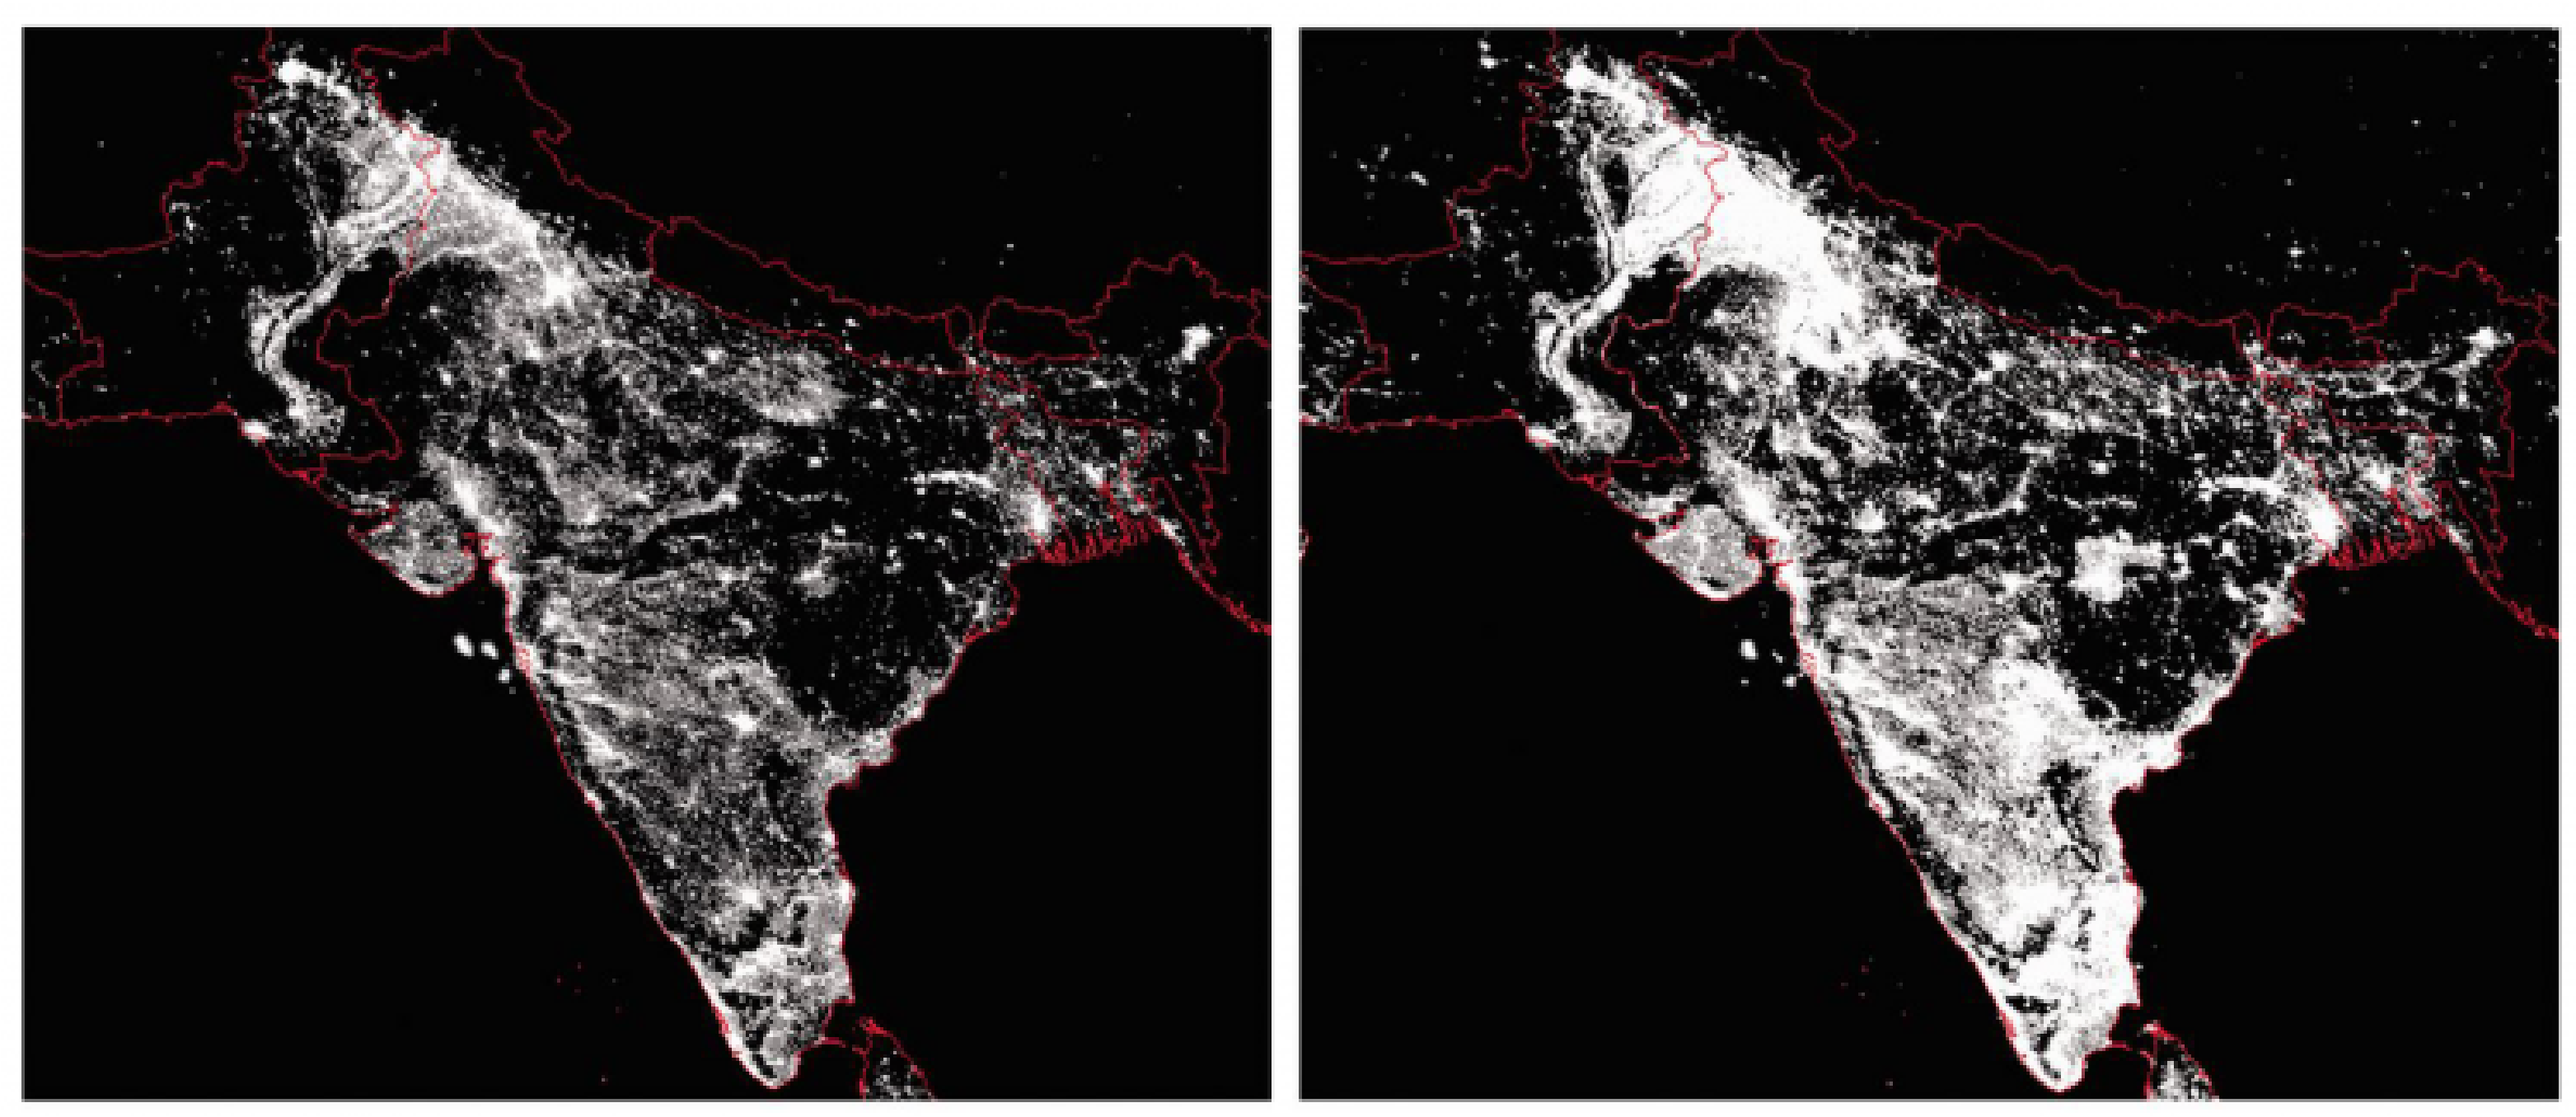
\includegraphics[width=0.6\linewidth]{/Users/alistairgj/Documents/GitHub/IoT_ResearchProject/IoT_November/images/satelliteImages} 

}

\caption{Satellite images of South Asia by night. Left (South Asia in 1994) Right (South Asia in 2010). Images are taken from Maxim Pinkovskiy and Xavier Sala-i-Martin (2016) - Lights, Camera ... Income! Illuminating the National Accounts-Household Surveys Debate. The Quarterly Journal of Economics.}\label{fig:satelliteImagesAsia}
\end{figure}

\begin{figure}[H]

{\centering 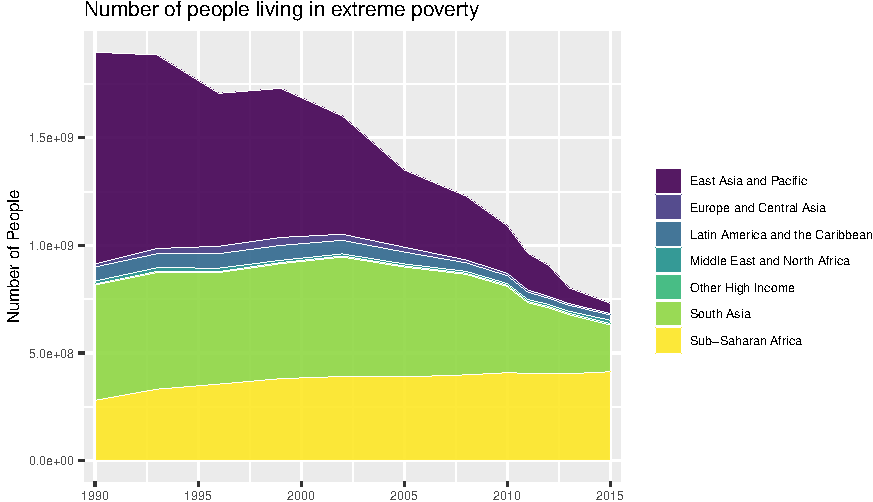
\includegraphics{MD_Final_files/figure-latex/globalPovertyPlot-1} 

}

\caption{The number of people living in extreme poverty between the years of 1990 till 2015, segmented by region. Source: The World Bank}\label{fig:globalPovertyPlot}
\end{figure}

\hypertarget{the-rise-and-rise-of-the-world-wide-web}{%
\subsubsection{The Rise and Rise of the World Wide
Web}\label{the-rise-and-rise-of-the-world-wide-web}}

According to the International Telecommunication Unions (\textbf{ITU})
2015 figures, Internet penetration has grown from just over 400 millions
users (6 per cent of global population) in 2000 to 3.2 billion users in
2015 (43 per cent of global population). This includes around 2 billion
users from developing countries
{[}\protect\hyperlink{ref-duttaGlobalInformationTechnology2015}{2}{]}.
ICTs bring a broad range of benefits and are recognised as a key to
eradicating poverty and unemployment. They enable and facilitate the
building of a people-centred, inclusive and development-oriented
Information Society, where everyone can create, access, utilise and
share information and knowledge. This enables individuals, communities
and peoples to achieve their full potential in promoting their
sustainable development and improving their quality of life
{[}\protect\hyperlink{ref-InformationCommunicationTechnologies}{3}{]}.
In addition to a rapidly growing internet user-base both in the
developing and developed world, the nature of internet usage has
fundamentally changed. Once the purview of academics, engineers and
computer scientists sending tiny packets of information back and forth,
there are now some 2.5 quintillion bytes of data created each day by all
manner of users, industries and sensors, to name a few
{[}\protect\hyperlink{ref-DataNeverSleeps}{4}{]}.

\begin{figure}[H]

{\centering 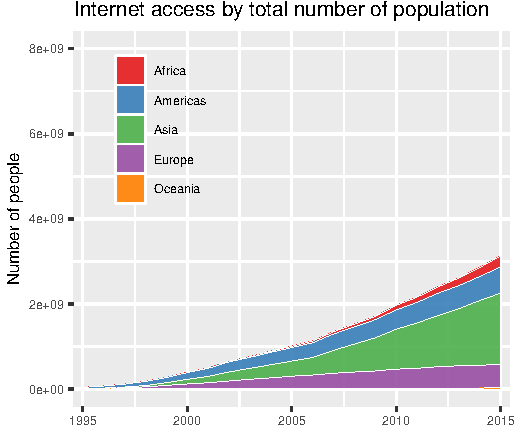
\includegraphics{MD_Final_files/figure-latex/internetAccessPlot-1} 

}

\caption{Internet access by total number of population, Source: The World Bank, World Development Indicators}\label{fig:internetAccessPlot}
\end{figure}

\hypertarget{forging-a-new-technological-paradigm}{%
\subsubsection{Forging a New Technological
Paradigm}\label{forging-a-new-technological-paradigm}}

Such rapid and widespread internet adoption has created a seemingly
insatiable demand for exponentially greater computational power and
digital storage capacity. This has led to a new and ubiquitous
technological paradigm: Cloud Computing. Cloud Computing is succinctly
defined as; the practice of using a network of remote servers hosted on
the Internet to store, manage, and process data, rather than a local
server or a personal computer
{[}\protect\hyperlink{ref-CloudComputingDefinition}{5}{]}.

As with the initial rise and widespread implementation of the Internet,
Cloud Computing itself acts as a facilitator for new technologies. One
such example being the Internet of Things (\textbf{IoT}) paradigm. The
IoT can be surmised as the extension of the Internet and the Web into
the physical realm, by means of the widespread deployment of spatially
distributed devices with embedded identification, sensing and/or
actuation capabilities, allowing objects to be sensed or controlled
remotely through the internet
{[}\protect\hyperlink{ref-danielemiorandiInternetThingsVision2012}{6}{]},
{[}\protect\hyperlink{ref-binghuangServiceOrientedComputing16th2018}{7}{]},
{[}\protect\hyperlink{ref-luigiatzoriInternetThingsSurvey2010}{8}{]}.
IoT thus represents a convergence of real-world objects and digital
objects into a unified cyber-physical system.

\hypertarget{the-bigger-picture}{%
\subsubsection{The Bigger Picture}\label{the-bigger-picture}}

Considering the bigger picture of societal benefit, as seen in figure
\ref{fig:globalPovertyPlot}, from 1990 through 2015 the number of people
living in extreme poverty has dropped by more than half. As evidenced by
Figure \ref{fig:internetAccessPlot}, over the same time period, the
percentage of people with access to the internet has move from around 1
per cent to an average of around 50 per cent (this trend is now moving
exponentially as a function of time). And, figure
\ref{fig:populationGrowthPlot} shows that over the last 100 years, the
human population has experienced unprecedented growth from 1 billion
individuals to in excess of 7 billion. Mankind have thus simultaneously
increased our population, increased of technological development and
decreased poverty (to name but a few, `key performance indicators').

\begin{figure}[H]

{\centering 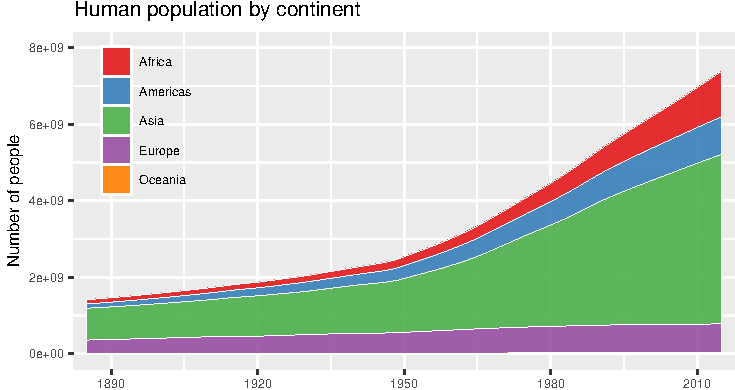
\includegraphics{MD_Final_files/figure-latex/populationGrowthPlot-1} 

}

\caption{Human population by continent, Source: The World Bank, World Development Indicators}\label{fig:populationGrowthPlot}
\end{figure}

The success of modern human society is not without consequence. All of
the benefits our society has enjoyed from the development, production
and deployment of technology, has required vast amounts of energy. This
energy has, since the industrial revolution, primarily been derived from
the burning of fossil fuels, as illustrated by Figure
\ref{fig:globalEnergyPlot}.

\begin{figure}[H]

{\centering 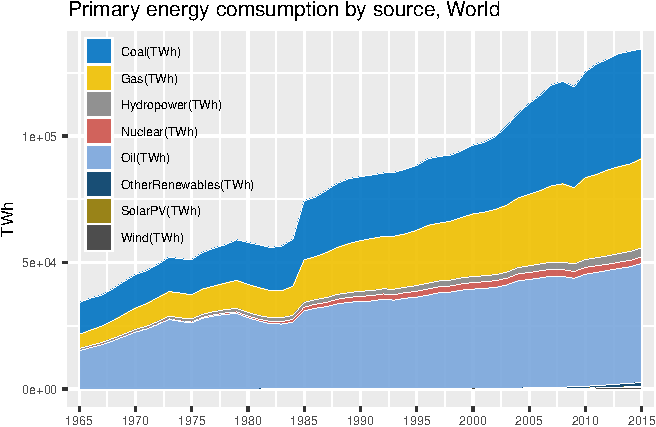
\includegraphics{MD_Final_files/figure-latex/globalEnergyPlot-1} 

}

\caption{ADD TEXT, Source: Our World in Data}\label{fig:globalEnergyPlot}
\end{figure}

The International Panel on Climate Change (IPCC) finds that Human
activities are estimated to have caused approximately 1.0°C of global
warming above pre-industrial levels, with a likely range of 0.8°C to
1.2°C. Global warming is likely to reach 1.5°C between 2030 and 2052 if
it continues to increase at the current rate
{[}\protect\hyperlink{ref-intergovernmentalpanelonclimatechangeGlobalWarming2018}{9}{]}.

Climate change poses an existential threat to modern human civilisation,
with warming of between 1.5°C and 2°C predicted to cause increases in
mean temperature in most land and ocean regions, hot extremes in most
inhabited regions and heavy precipitation changes in some regions.
Additionally, increases in ocean temperature as well as associated
increases in ocean acidity and decreases in ocean oxygen levels are
projected to reduce risks to marine biodiversity, fisheries, and
ecosystems, and their functions and services to humans. Taken together,
these effects will lead to risks of the health, livelihoods, food
security, water supply, human security, and economic growth of mankind
{[}\protect\hyperlink{ref-intergovernmentalpanelonclimatechangeGlobalWarming2018}{9}{]}.

\begin{figure}[H]

{\centering 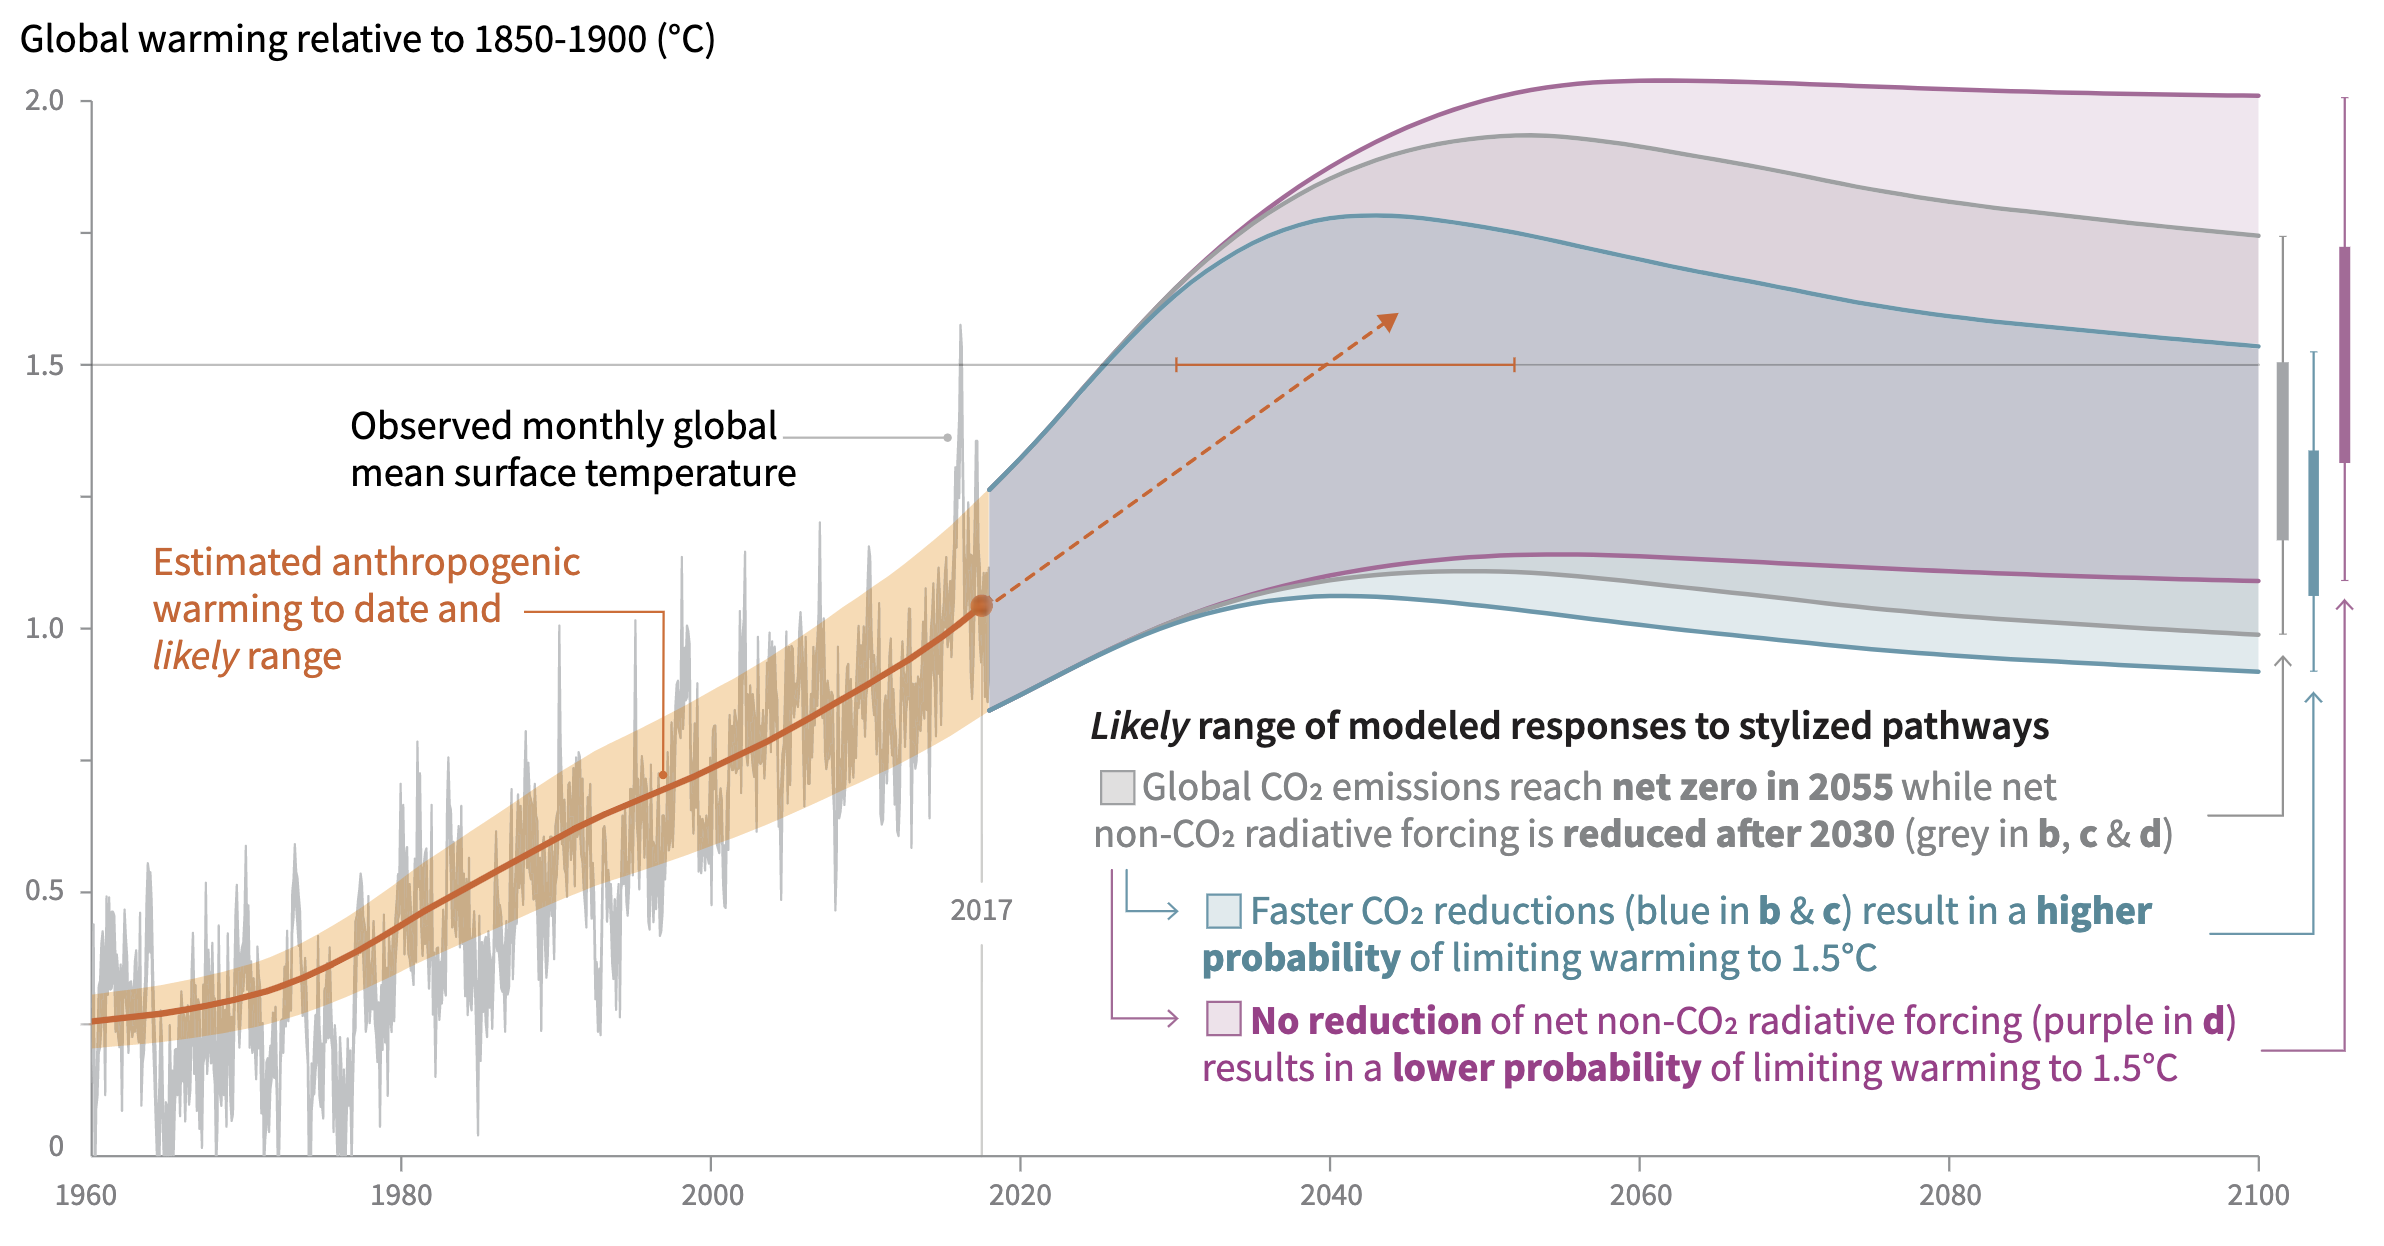
\includegraphics[width=0.8\linewidth]{/Users/alistairgj/Documents/GitHub/IoT_ResearchProject/IoT_November/images/warmingTrend} 

}

\caption{Atmospheric Changes with respect to Carbon Emissions and Global Warming - Observer and Projected. Source: Intergovernmental Panel on Climate Change, 2018}\label{fig:warmingTrend}
\end{figure}

It is therefore imperative moving forward as a species that all steps
are be taken to mitigate the emission of greenhouse gases and abate the
advance of anthropomorphic climate change. The scale of the challenge is
such that technology itself will prove critical in effectively combating
this existential threat to civilisation. When considering energy
consumption, the industrial sector (including the non-combusted use of
fuels) currently consumes around half of all global energy and feedstock
fuels, with residential and commercial buildings (29\%) and transport
(21\%) accounting for the remainder
{[}\protect\hyperlink{ref-EnergyDemandSector}{10}{]}

\begin{figure}[H]

{\centering 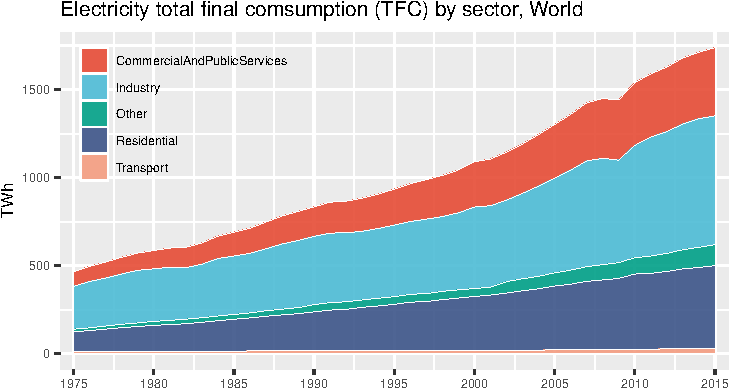
\includegraphics{MD_Final_files/figure-latex/sectorEnergyPlot-1} 

}

\caption{ADD TEXT}\label{fig:sectorEnergyPlot}
\end{figure}

\hypertarget{optimising-global-energy-usage}{%
\subsubsection{Optimising Global Energy
Usage}\label{optimising-global-energy-usage}}

Thus far, our staggering global achievements, including lifting hundreds
of millions out of poverty, rapid global technological deployment and
strong population growth has been inexorably linked to increased energy
consumption. This in turn has led to perturbations in atmospheric
chemistry, in the form of anthropogenic climate change (amongst many
other environmental challenges), which fundamentally threatens our
global achievements. It therefore stands that the key to continued human
prosperity is to de-couple growth in energy demand from economic growth.
In this work we will explore the possibility of reducing energy
consumption via the optimization of services to end users in an IoT
Smart Home.

\hypertarget{the-iot-smart-home-service-oriented-computing}{%
\subsubsection{The IoT Smart Home \& Service Oriented
Computing}\label{the-iot-smart-home-service-oriented-computing}}

As mentioned above, residential and commercial buildings account for
29\% of energy demand globally
{[}\protect\hyperlink{ref-Consumption}{11}{]}. In this work we propose
that an avenue for reduced energy consumption is the optimization of
existing services and utilities to end users in an IoT Smart Home. In
this proposed smart home, the daily activities of the end user can be
performed with the support of a personalised artificial intelligence
(AI) system, such that the timing and manner of energy intensive
activities is optimised to reduce overall energy consumption, whilst
still considering the level of convenience afforded to the end user.
This work uses sensor data analogous to what would be expected to be
produced from a sensor rich IoT smart home and considers the interplay
between end user convenience; predictive analytics; predictive service
offering; energy consumption; demand response and smart electricity
grids.

\hypertarget{aim}{%
\subsection{Aim}\label{aim}}

\hypertarget{research-questions}{%
\subsubsection{Research Questions}\label{research-questions}}

The aim of this work is to use sensor data from X to consider Y in the
context of Z.

\hypertarget{research-contributions}{%
\subsubsection{Research Contributions}\label{research-contributions}}

The aim of this work is to use

\pagebreak

\hypertarget{preliminaries}{%
\section{Preliminaries}\label{preliminaries}}

Significant growth in digital interconnectivity over the last 20 years
has given the internet a pivotal role as an essential element of
economic growth
{[}\protect\hyperlink{ref-haseebDoesInformationCommunication2019}{12}{]}.
Cloud computing and the IoT paradigm has enabled the association of
previously disparate fields into a larger coherent framework. Namely,
smart home appliances, demand-response, energy consumption, predictive
analytics predictive service offering and end user convenience. This
work proposes a framework for the association of sensor data into a
model which can do X Y Z. \textbf{Mention internet in general?}

\hypertarget{related-work}{%
\subsection{Related Work}\label{related-work}}

\hypertarget{ubiquity-of-the-world-wide-web-and-implications-for-energy-consumption}{%
\subsubsection{Ubiquity of the World Wide Web and Implications for
Energy
Consumption}\label{ubiquity-of-the-world-wide-web-and-implications-for-energy-consumption}}

The International Telecommunication Union estimated about 3.2 billion
people, or almost half of the world's population, would be online by the
end of the 2015
{[}\protect\hyperlink{ref-InformationCommunicationTechnologies}{3}{]}.
The impact of internet usage and mobile cellular subscriptions
(\textbf{ICTs}), globalization, electricity consumption, financial
development, and economic growth on environmental quality has been
examined
{[}\protect\hyperlink{ref-haseebDoesInformationCommunication2019}{12}{]}.
By using 1994--2014 panel data of the Brazilian, Russian, Indian,
Chinese \& South African (\textbf{BRICS}) economies, empirical results
demonstrate that rise in both internet usage and mobile cellular
subscription ICTs likely mitigates CO2 emissions.

\textbf{BRIDGE} -- Greater internet availability / connectivity
facilitates the deployment of smart electricity grids

\hypertarget{smart-metering}{%
\subsubsection{Smart Metering}\label{smart-metering}}

A Smart meter is an electronic device that records consumption of
electric energy and communicates the information to the electricity
supplier for monitoring and billing. In the Unites States (for example)
smart meters are a significant part of the larger Smart Grid
infrastructure, and as far back as 2012, had been installed in over 25
million U.S. homes
{[}\protect\hyperlink{ref-hornePrivacyTechnologyNorms2015}{13}{]}. Smart
Meters transmit information about consumer electricity use to utility
companies at vastly shorter time intervals than before and this
information helps utility companies to coordinate power supply and
demand, detect outages, implement time-of-use and dynamic pricing, and
in other ways improve system efficiency and reliability. Additionally,
these data are also becoming increasingly available, and sought-after,
by end-users themselves. Indeed, the main purpose of provisioning smart
metering data to end users is to encourage the use of less electricity,
by better informing users of their consumption patterns
{[}\protect\hyperlink{ref-jui-shengchouCloudForecastingSystem2019}{14}{]}.
In the aggregate, these savings can significantly reduce national energy
use and curb energy emissions while addressing pressing geopolitical and
environmental concerns related to energy security and sustainability
{[}\protect\hyperlink{ref-graabSmartGridSmart2011}{15}{]}.

Since the widespread deployment of smart meter technology, there has
been huge interest in the capability of these technologies with respect
to the technical capacity of utility companies to manage demand (through
demand response programs), incorporate renewable sources of electricity
into the system, and increase the overall efficiency and reliability of
the system
{[}\protect\hyperlink{ref-hornePrivacyTechnologyNorms2015}{13}{]}.
\textbf{It is worth noting, however, that the scenario described above
relies on end user intervention.}

\hypertarget{electricity-demand-response-smart-electricity-grids-and-smart-home-data}{%
\subsubsection{Electricity Demand Response, Smart Electricity Grids and
Smart Home
Data}\label{electricity-demand-response-smart-electricity-grids-and-smart-home-data}}

Predicting and influencing residential energy use has been the subject
to extensive study (\textbf{REF}). Literature indicates that factors
such as occupant behaviour and socio-economic status are important
\textbf{{[}15 from Cetin{]}}. Nielsen attributed 36\% of variation in
energy consumption of homes to lifestyle and occupant behaviour, and
64\% to socio-economic influences. This is exemplified by the work of De
et al, who show that in developing nations, cooking consumes up to 90\%
of the overall residential energy consumption and is mainly based on
non-renewable energy (International Energy Agency, 2006; De et al.,
2013). Other factors such as climate zone, number of occupants, income
level, age of home, and size of home have also been correlated with home
energy use (K.S. Cetin, 2014). The has been much work both on using
smart meter data to evaluate consumer behaviour, and the interplay
between smart appliances and shifting households' electricity demand.

Kavousian et al identify the need for developing an analytical method
that can leverage 15-minute or 30-minute interval energy consumption
data produced via smart metering in order to improve the effectiveness
of energy efficiency programs. They note that utilities spend millions
of dollars annually to improve appliance energy efficiency. By way of
example, in 2013 utilities in California US spent \$80 M USD on
appliance and plug load efficiency programs, the highest expenditure
among all utility energy efficiency programs (\textbf{CPUC, 2013 FIND
REF}). A need for analytical methodologies that can process smart meter
data and allow energy reduction savings to be identified is
demonstrated. Using a smart meter dataset of 4231 households, containing
information on electricity consumption at 30-minute intervals, with
aggregated local weather data, the authors use smart meter data to rank
residential appliance efficiency. Various control methodologies are
embedded into the analytical process, taking into account building type,
building size (e.g., apartment, detached), household type (e.g., de
facto, single, dependents), respondent age and heater type (e.g.,
electric or gas). The data set included 120+ household variables, many
of which were highly correlated, model selection techniques were used to
successfully reduce dimensionality. A set of load profiles were compiled
based on the results (where normalized load was plotted as a function of
hour of day). It was determined that household behaviour and demographic
can be used to generate positive and negative energy efficiency
coefficients with respect to load profiles. This work has implications
for energy grid planning -- for example in high-density housing versus
suburban housing.

Karjalainen considers the manner in which smart meter data is
communicated to end users, with the principal purpose of the paper being
to study what kind of electricity consumption feedback consumers
understand and prefer (Karjalainen, 2011). It is noted that the most
effective feedback tools for engaging households in reducing energy
consumption are both computerized and interactive. In this work a series
of options for feedback is gathered, for example consumption (kHh),
power (W), cost (\$), environmental impact (e.g., kg CO2), total for
household, disaggregation by appliance, real time, hour, day, and so on.
Examples of feedback options are shown in Figure \textbf{X}, below.

\begin{figure}[H]

{\centering 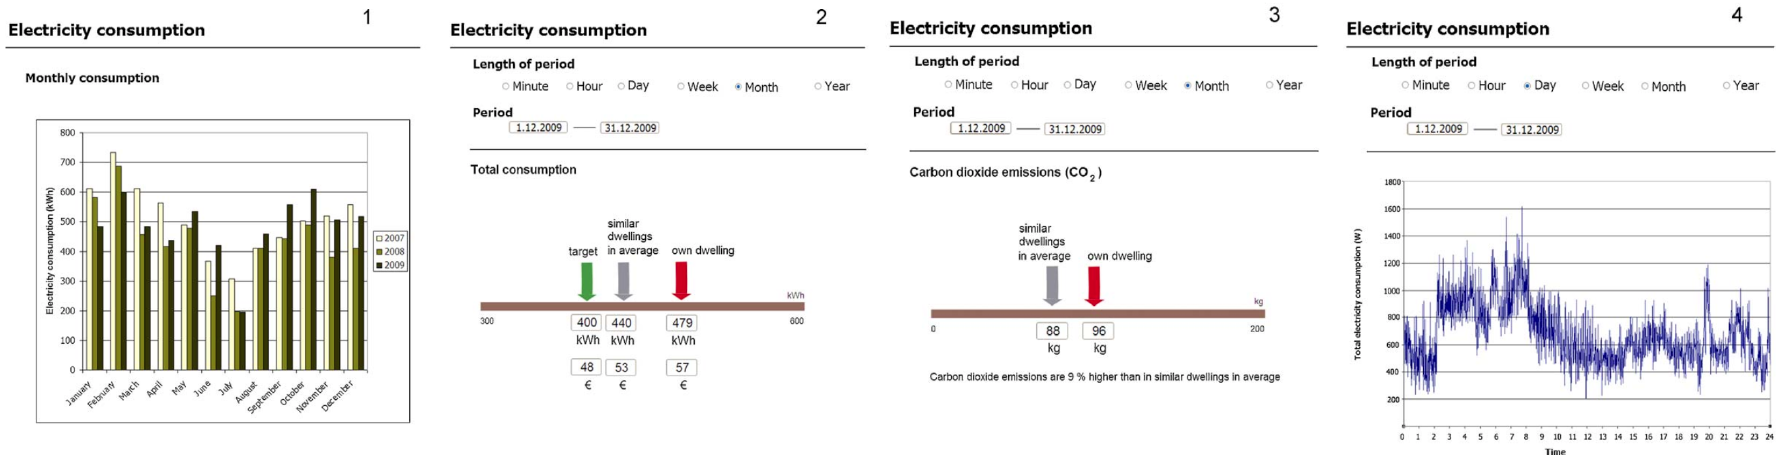
\includegraphics[width=1\linewidth]{/Users/alistairgj/Documents/GitHub/IoT_ResearchProject/IoT_November/images/dash1234} 

}

\caption{ADD TEXT}\label{fig:unnamed-chunk-1}
\end{figure}

\begin{figure}[H]

{\centering 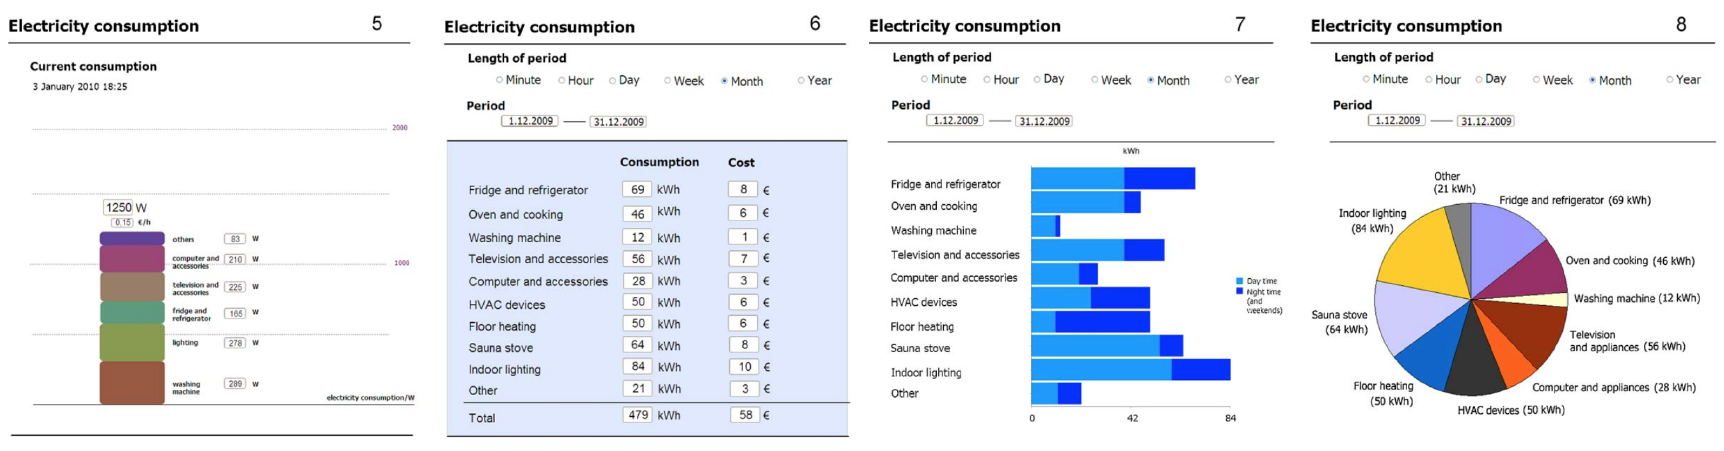
\includegraphics[width=1\linewidth]{/Users/alistairgj/Documents/GitHub/IoT_ResearchProject/IoT_November/images/dash5678} 

}

\caption{Option Five, Six, Seven and Eight of the smart meter data dashboards proposed by Karjalainen}\label{fig:unnamed-chunk-2}
\end{figure}

The results of qualitative participant interviews clearly showed that
while some consumers are very interested in saving household
electricity, other consumers show only a little interest (\textbf{NOTE
they were asked about saving electricity, not about saving money or
convenience}). When specifically asked to list what measures (if any)
were typically taken at home to realize reductions in energy usage, some
respondents listed numerous measures, while others just said they turn
lights off in rooms that are empty. The author also found some
participants were unaware of differences in stand-by versus active modes
of operation for electrical appliances, resulting in practising
inefficient energy saving measures in the home environment. When
trialling feedback prototypes to participants, two main issues were
encountered: (1) many people are not familiar with scientific units and
do not understand the difference between W and kWh and (2) many people
do not understand how carbon dioxide emissions are related to
electricity consumption. It is perhaps surprising that the overall most
popular prototype was `6', below. Perhaps because unlike the other
prototypes, this clearly (the most clearly) articulates cost. The
concept of convenience was absent entirely from consideration.

In the domain of supply and demand economics, consumer behaviour and
smart appliances Kobus et al investigated if households can shift their
electricity demand to times when electricity is abundantly available
{[}\protect\hyperlink{ref-charlotteb.a.kobusReallifeAssessmentEffect2015}{16}{]}.
Using a household electrical monitoring system (\textbf{EMS}) coupled to
a smart appliance (smart washing machine), photovoltaic cells and the
electricity grid, they were able to show that households can shift
10--77\% of the electricity demand of their washing machine. This
longitudinal study was conducted via the participation of 50 Dutch
households over a period of one year. By utilizing an EMS which shows
appliance status, dynamic tariff information and current status of
household electricity usage, participants are able to schedule smart
washing machine use in such a way that cost is minimized.

\begin{figure}[H]

{\centering 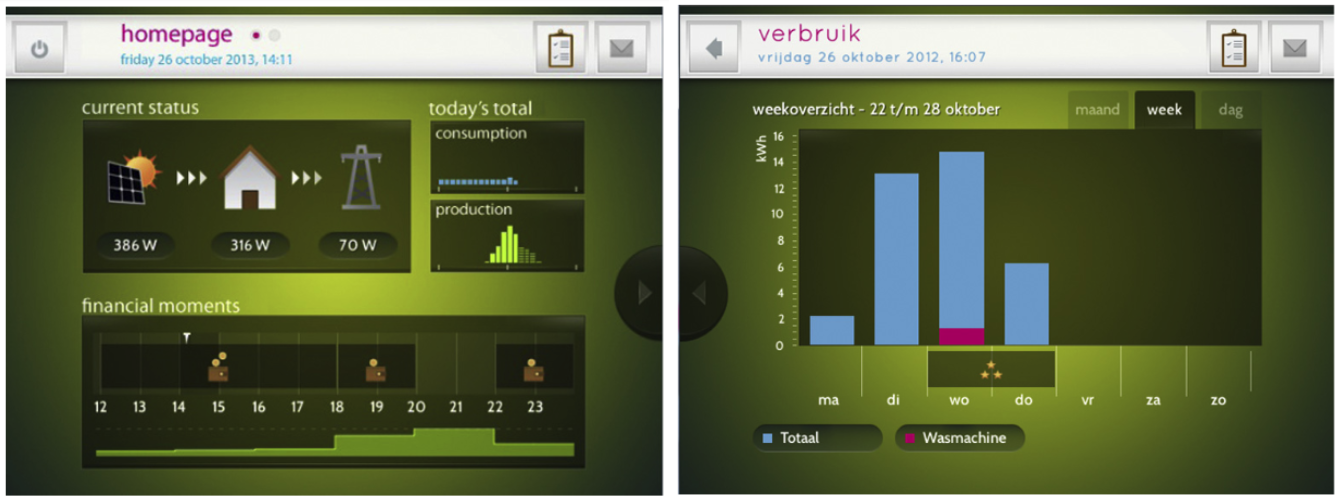
\includegraphics[width=0.6\linewidth]{/Users/alistairgj/Documents/GitHub/IoT_ResearchProject/IoT_November/images/kobusDash} 

}

\caption{ADD TEXT}\label{fig:unnamed-chunk-3}
\end{figure}

Their work is in response to two major challenges to domestic
electricity supply and demand. \textbf{REMOVED: It is well observed that
over electricity grids, demand shows a pattern over time, influenced by
natural and social circumstances. This poses a great challenge when
considering renewable energy sources like PV -- people are generally not
at home when local electricity is abundantly produced (for example the
daylight hours of Monday till Friday)} The first being that the amount
of distributed renewable electricity generation is increasing with time
(for example, as more households install photovoltaic (\textbf{PV})
panels), and the second that electricity demand will continue to
significantly increase moving into the foreseeable future. These
developments pose great challenges to `traditional' power systems, where
supply follows demand entirely. Smart grids are proposed as a potential
solution to facilitate the affordable introduction of cleaner
electricity producing and consuming technologies.

Cetin et al consider electricity usage of appliance, as when aggregated,
this accounts for approximately 30 per cent of electricity used in the
residential building sector
{[}\protect\hyperlink{ref-k.s.cetinApplianceDailyEnergy2014}{17}{]}.
This, together with small appliances, home electronics and lighting,
account for more than 2/3 of total residential electricity use. Cetin et
al also highlight that influencing `time of use' is becoming
increasingly important to control the stress on today's electrical grid
infrastructure. The authors seek to determine when refrigerators,
clothes washers, clothes dryers and dishwashers are predominantly used
(and thus consume energy) and what causes variation in their use. Using
disaggregated energy data from 40 homes over a period of 1-year,
normalized load profiles for the four target appliances were generated,
as a percentage of daily electricity load.

\begin{figure}[H]

{\centering 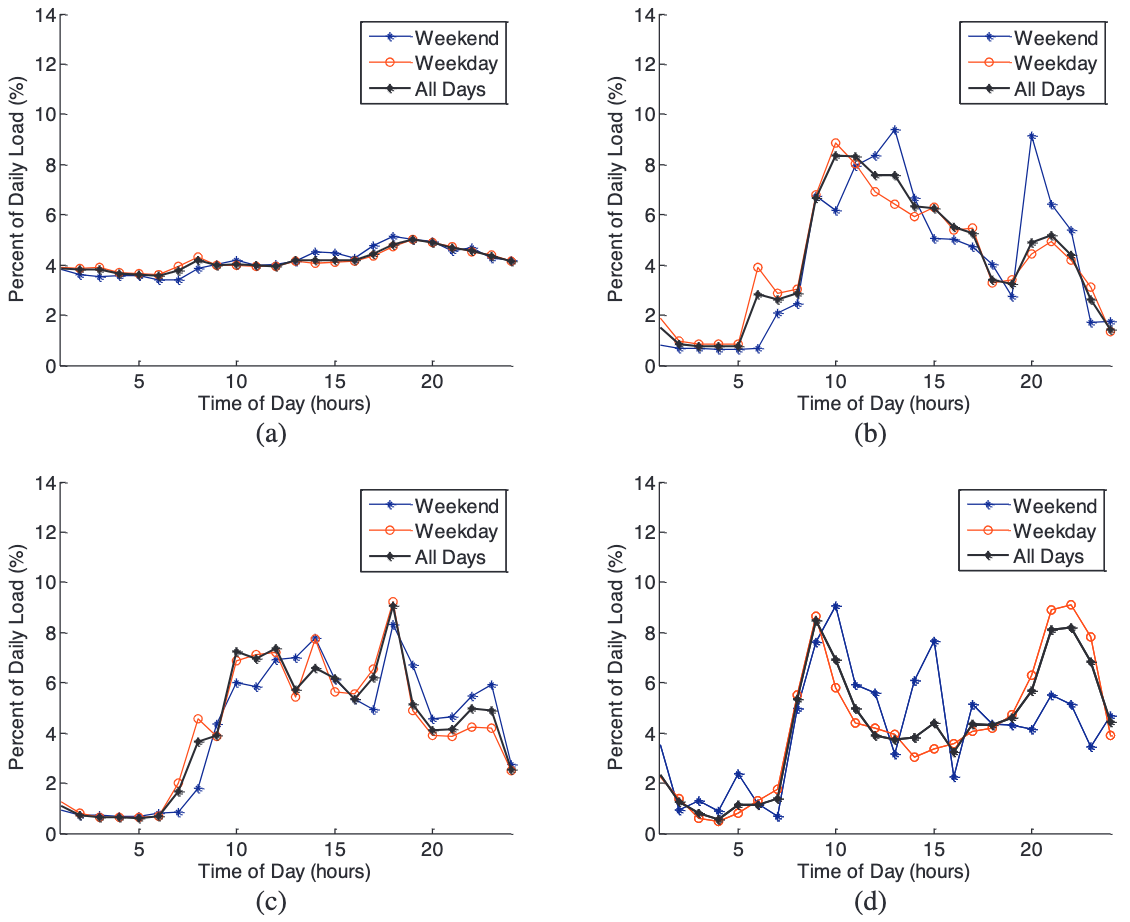
\includegraphics[width=0.65\linewidth]{/Users/alistairgj/Documents/GitHub/IoT_ResearchProject/IoT_November/images/cetinResults} 

}

\caption{ADD TEXT}\label{fig:unnamed-chunk-4}
\end{figure}

It was found that the refrigerator had the most consistent consumption
profile across all homes surveyed. Influencing factors for the
refrigerator were correlated to both indoor and outdoor temperature,
however effect was found to be minimal. The clothes washer and dryer
were found to have the greatest variation in normalised energy use by
hour, with the greatest period of use from 9am until 2pm. The dishwasher
had distinct peaks in load profile at 9am and 10pm. The authors found
that user-dependent appliance use patterns vary more between homes and
between days than automated appliances, weekday and weekend use patterns
of appliances are similar, and that electricity use varies more between
houses during peak use times of day than during low-use times. Murray et
al further explore the topic of home appliance energy consumption using
smart meter data, specifically pertaining to residential activities
around food storage and preparation (D.M. Murray, 2018), with the aim of
providing a model that can easily be applied to existing smart meter
energy datasets. The authors use real-time energy consumption data from
microwaves and ovens, from which user behaviour / desired outcome can be
implicitly associated (for example, oven usage on a weekday between the
hours of 6pm and 8pm can be associated with the behaviour of preparing
dinner). Consideration is given to the concept of the RisingEdge (when
an appliance is switched on or moves to a high consuming state) and
FallingEdge (when an appliance is switched off or moves to a low
consuming state) of power consumption. Accurate energy consumption
models for major cooking appliances are successfully constructed,
further re-enforcing the value and widespread applicability of
residential smart meter data.

In this work,

This supports \_\_ that smart meters represent a valuable source of data
that can be used for a variety of purposes, beyond just real-time
monitoring. For example the model constructed by Murray et al does not
rely on difficult to obtain parameters such as food type, temperature
and weight. it has been shown that \ldots{}

\begin{itemize}
\tightlist
\item
  Authors are able to use smart meter data to build accurate energy
  consumption models of major cooking appliances
\item
  Smart =
\item
  Using consumption data from real homes, the authors are able to create
  scalable mathematical models to account for energy consumption
  associated with food preparation
\item
  Indeed, from an energy-efficiency perspective, targeted energy
  feedback can be provided on consumers appliance usage habits and
  activities (Stankovic et al., 2016) leading to informed energy savings
  programmes and retrofit strategies for replacing appliances.
\item
  And if this variation can be influenced??
\end{itemize}

\emph{Demand Response allows for the management of demand side resources
in real-time; i.e.~shifting electricity demand according to fluctuating
supply. When integrated into electricity markets, Demand Response can be
used for load shifting and as a replacement for both control reserve and
balancing energy. These three usage scenarios are compared based on
historic German data from 2011 to determine that load shifting provides
the highest benefit: its annual financial savings accumulate to €3.110M
for both households and the service sector. This equals to relative
savings of 2.83\% compared to a scenario without load shifting.}

{[}{\textbf{???}}{]} discuss electricity demand response - allowing the
management of demand side resources in real-time. \textbf{Based on Darby
and McKenna (REF), we define demand response and a household action
(automated, manual, or both) due to which electricity use is shifted in
time in response to a price signal of other stimuli. This can result in
more efficient usage of the available sustainable electricity, like
self-consumption of on-site PV electricity (REF) and peak demand
reductions (REF) - all from \textbf{???}\{kobus2015\}}

\hypertarget{predictive-modelling-and-forecasting}{%
\subsubsection{Predictive Modelling and
Forecasting}\label{predictive-modelling-and-forecasting}}

In the domestic predictive energy consumption space Basu et al consider
home automation systems linked via a communication network to enable
interaction, data collation and control of appliances remotely by end
users
{[}\protect\hyperlink{ref-kaustavbasuApplianceUsagePrediction2012}{18}{]}.
The potential competing priorities of energy savings versus comfort
optimization for home occupants is discussed. The objective of this work
is to propose a learning system that is able to help the home automation
system compute an energetic plan that is also satisfactory to user
requests. Taking into account correlation between appliances, a
time-series based multi-label classifier is used to predict appliance
usage up to one hour into the future.

The attribute construction technique of Knowledge Extraction applied.
This process aims to extract novel attributes from underlying
substructures in the training instances in the form of sub-events, for
example periodicity in data. This Knowledge Extraction process is
similar to the implicit associations used by Murray et al, in the
analysis of energy consumption for food preparation
{[}\protect\hyperlink{ref-d.m.murrayApplianceElectricalConsumption2018}{19}{]}.
The substructures are then fed to a propositional learner. The proposed
model is trained in an iterative manner and attempts to take into
account all the possible information based on consumption data, time of
the event and meteorological information. Time is specifically model
time as a periodic variable, segmenting on hour of day and day of week,
noting that this takes into account the periodic nature of human
behaviour. Using BR1, LP, CC1, CC2 and MLk machine learning algorithms,
the precision, recall and accuracy for a variety of
electricity-consuming appliances is determined (where each appliance
constitutes a target variable over a set of iterations). In the
evaluation phase they find that user behaviour toward an appliance is
highly variable and the predictability of an appliance is dependent on
the regularity of usage patterns of the inhabitants. It is specifically
noted that \emph{it is therefore very difficult for now to propose a
generic methodology of appliance prediction for private houses}.

\begin{figure}[H]

{\centering 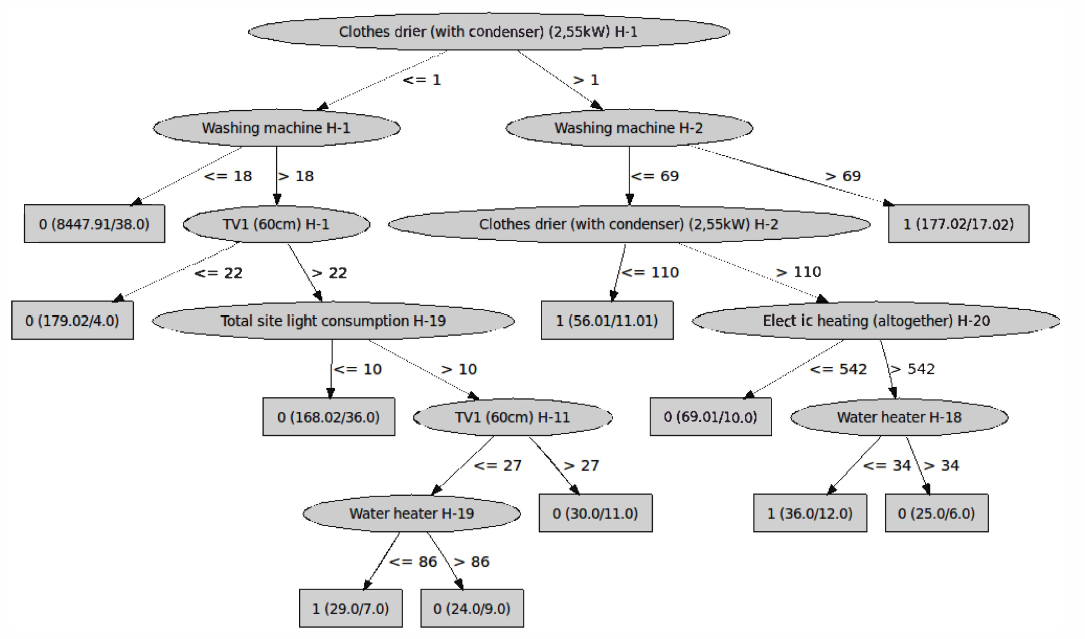
\includegraphics[width=0.8\linewidth]{/Users/alistairgj/Documents/GitHub/IoT_ResearchProject/IoT_November/images/basuTree} 

}

\caption{ADD TEXT}\label{fig:unnamed-chunk-5}
\end{figure}

Chou et al consider global energy consumption in the residential housing
sector in the context of domestic energy information system (EIS) and
smart meter system (smart grids) technologies
{[}\protect\hyperlink{ref-jui-shengchouCloudForecastingSystem2019}{14}{]}.
They note two influential factors on overall residential energy
consumption, the first being the type and number of electrical
appliances and the second being the usage of these appliances by
occupants. It is proposed that a major challenge for people who are
willing to save energy at home is a lack of information about their
energy consumption. To test this hypothesis, the authors develop a
web-based energy information management system for the power consumption
of home appliances that monitors the energy load of a home, analyses its
energy consumption based on machine learning, and then sends information
to various stakeholders. Interaction with end-users in the home is
achieved via energy dashboards and emails. The authors propose that
end-users of this system can use forecast information and anomalous data
to enhance the efficiency of energy usage in their buildings especially
during peak times by adjusting the operating schedule of their
appliances and electrical equipment. \textbf{In order to achieve the
desired model (???)}

During this study, an EIS with 5 main components was installed in an
experimental building. The parts were as follows; (1) the internal
communication network, (2) the data management infrastructure, (3) the
automated prediction system, (4) the web-based system and dashboard and
(5) the early warning system. Data from both the smart meter and from
sensors was used to compile the model, including timestamps (YYYY-MM-DD
hh:mm:ss), outdoor temperature (ºC), total building energy consumption
(kWh), aggregated energy consumption data (e.g., second floor lighting)
and individual appliances. The backend of the application was notably
cloud-hosted.

\begin{itemize}
\tightlist
\item
  Improve consumer satisfaction by providing real-time services that
  enable end-users to monitor the energy consumption easily.
\item
  Energy Information System - personalised terminal in domestic home
  which provides real-time or daily updating of hourly energy
  consumption data allows users to address building performance issues
  that are otherwise difficult to identify.
\item
  The data stream from the smart meters arrives at 15 min intervals,
  generating 96 data points daily for each smart meter.
\item
  The hardware of the DBMS consists of the communication system, the
  smart meter system, the environmental sensor system, and the server
  system, and the software programs that are used to process the data
  written in MATLAB. A DBMS stores real-time data that are retrieved
  from the smart grid metering infrastructure, including real-time
  energy consumption data, information about appliances, data from
  temperature and humidity sensors, and analytical results, including
  predicted electricity consumption, and data on electricity-saving
  alternatives. Moreover, the DBMS stores electrical parameters such as
  voltage, current, power, frequency, and power factor.
\item
  The proposed prediction model (i.e.,SARIMA-MetaFA-LSSVR) consists of
  stage 1, involving univariate linear technique, and stage 2, involving
  optimized multivariate nonlineartechnique tofit the energy consumption
  data. SARIMA is adopted to handle the linear component, whereas Meta
  FA-LSSVR is used to model the nonlinear part of energy consumption
  data. In particular, the MetaFA is employed for automatically tuning
  LSSVR hyper parameters, thus improving the overall prediction
  performance.
\item
  Output
\item
  A web-based system to display energy consumption that is measured in
  real time with previously predicted values.
\item
  Early-warning system integrated into web-based system to detect
  anomalous power consumption and provide warnings (notifications)
  thereof to users.
\item
  The real-time prediction model in web-based system is designed and
  implemented based on our previous work{[}20,33,49{]}, which developed
  a novel sliding window metaheuristic optimization-based machine
  learning system to analyze time-series data that are generated by a
  smart grid to efficiently forecast energy consumption one day in
  advance.
\end{itemize}

\hypertarget{smart-home-and-energy-efficiency}{%
\subsubsection{Smart Home and Energy
Efficiency}\label{smart-home-and-energy-efficiency}}

{[}{\textbf{???}} NOT IN LIB{]} - As recently as 2009 it was posited
that ``The proposed model allows for introduction of power priorities
for consumer's electrical equipment by the importance of their
functions. The relevance of the functions carried out by the data device
is evaluated by each consumer individually. The relevance of functions
and priorities assigned to power mode / groups of electrical equipment
can be changed over time.''\\
`Haseeb et al {[}{\textbf{???}} NOT IN LIB{]} have (through review)
shown that at a macro scale, global adoption of internet reduces energy
consumption' + At the micro scale (that is, the behaviour of
individuals\ldots)

\hypertarget{iot-and-end-user-convenience}{%
\subsubsection{IoT and End User
Convenience}\label{iot-and-end-user-convenience}}

The term Internet-of-Things (\textbf{IoT}) is used as an umbrella
keyword for covering various aspects related to the extension of the
Internet and the Web into the physical realm, by means of the widespread
deployment of spatially distributed devices with embedded
identification, sensing and/or actuation capabilities
{[}\protect\hyperlink{ref-danielemiorandiInternetThingsVision2012}{6}{]}.
The IoT paradigm is fundamental to this work, representing the
confluence of multiple technological advancements
{[}\protect\hyperlink{ref-luigiatzoriInternetThingsSurvey2010}{8}{]}
including, ubiquity of internet access, the availability of
high-performance internet connectivity, inexpensive consumer electronics
with embedded sensing and control systems, automation, real-time
analytics, machine learning, commodity sensors and embedded systems. In
the IoT paradigm, digital and physical entities can be linked, by means
of appropriate information and communication technologies, to enable a
whole new class of applications and services
{[}\protect\hyperlink{ref-danielemiorandiInternetThingsVision2012}{6}{]}.

One consequence resulting from the widespread deployment of consumer
electronics with IoT capability is the evolution of the Internet from
interconnecting computers to interconnecting things. Figure X, below,
shows XYZ.

\begin{figure}[H]

{\centering 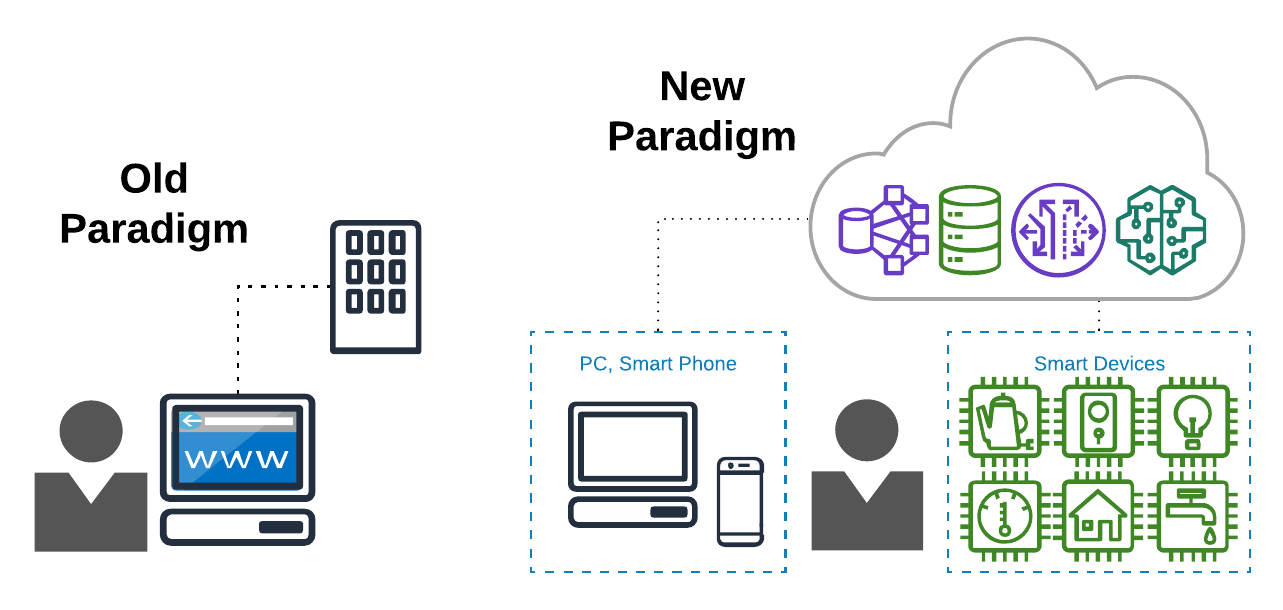
\includegraphics[width=0.65\linewidth]{/Users/alistairgj/Documents/GitHub/IoT_ResearchProject/IoT_November/images/oldNewParadigm} 

}

\caption{ADD TEXT}\label{fig:unnamed-chunk-6}
\end{figure}

\hypertarget{heading}{%
\subsubsection{Heading???}\label{heading}}

Huang et al propose a novel service mining framework to personalize
services in an IoT-based smart home (Bing Huang, 2018). This work
considers the notion of personal `convenience' as a driving force behind
the provisioning of services to end users. That is, in an IoT smart
home, where everything is interconnect, can services (for example, the
switching on or off of a light) be automatically served to users such
that their level of effort (to interact with their surroundings) will be
diminished, and thus their level of convenience will be increased?

\begin{figure}[H]

{\centering 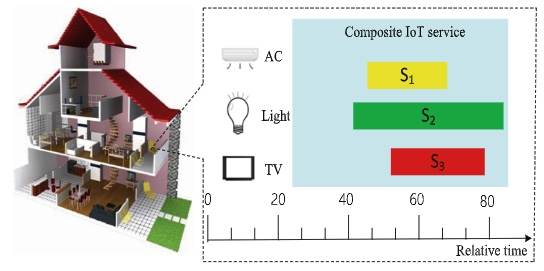
\includegraphics[width=0.5\linewidth]{/Users/alistairgj/Documents/GitHub/IoT_ResearchProject/IoT_November/images/huangA} 

}

\caption{ADD TEXT}\label{fig:unnamed-chunk-7}
\end{figure}

Using this framework, IoT services can be composed in a periodic
fashion, for the convenience of the end user / consumer.

\begin{itemize}
\tightlist
\item
  Use intelligence to compose IoT services for the convenience of the
  end user / consumer
\end{itemize}

The input for this work was data from domestic IoT services, with a
corresponding timestamp. The end user in this scenario performs daily
activities by interacting with IoT services, these interactions are
recorded as IoT service event sequences. A novel PCMiner algorithm
(Periodic Composite IoT Service Miner)

Periodic composite IoT services can be loosely defined as the composite
IoT services' repeating occurrence at certain locations with regular
time intervals

The output for this work was an IoT service model and a composite IoT
service model (based on spatio-temporal features). A periodic composite
IoT service model to represent the regularity of composite IoT services
occurring at a certain location at a certain time interval

\begin{figure}[H]

{\centering 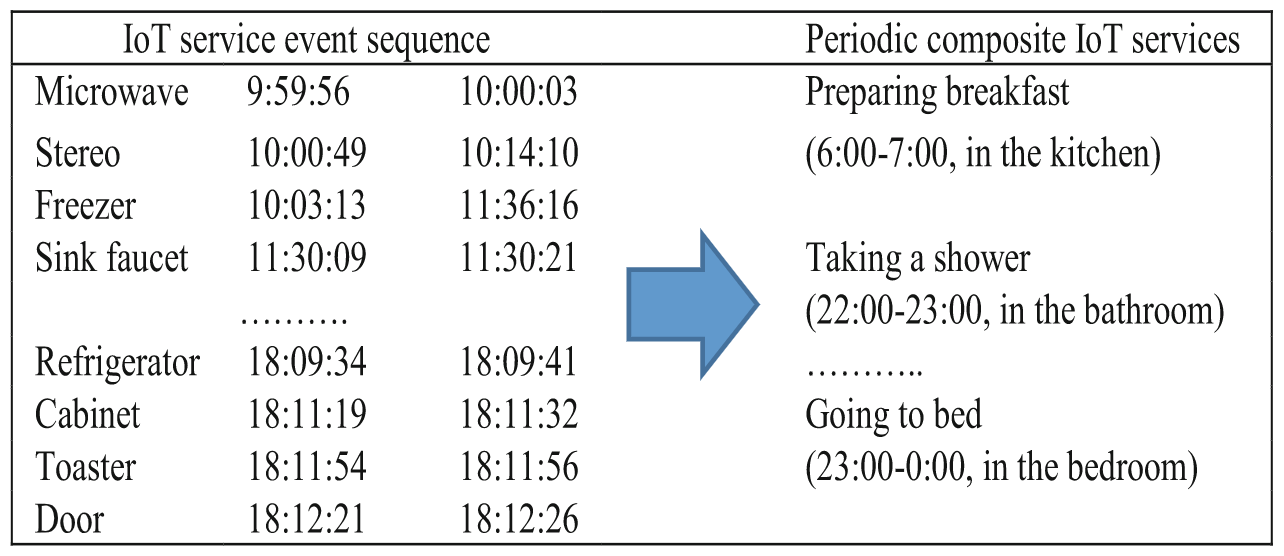
\includegraphics[width=0.5\linewidth]{/Users/alistairgj/Documents/GitHub/IoT_ResearchProject/IoT_November/images/huangC} 

}

\caption{ADD TEXT}\label{fig:unnamed-chunk-8}
\end{figure}

Critical to note that in this work model composition is reliant on
temporal, proximity and duration features.

Output: Spatio-temporal proximity model

\begin{itemize}
\tightlist
\item
  Filter out insignificant spatio-temporal IoT service relationships
  Categories (e.g., objective):
\item
  Quantify the correlation strength of among IoT services from time and
  location aspects
\item
  IoT devices are highly heterogeneous in terms of supporting
  infrastructure ranging from networking to programming abstraction
\item
  Hiding (abstracting) complex and diverse supporting infrastructure
\item
  Proximity and correlation strength
\end{itemize}

Service Mining on the Web \textbf{???}\{zheng2009\}

In the domain of Service Mining and Service Recognition, Zheng et al aim
to provide end users with value-added services through the composition
of existing services (output = composed web services). They attempt to
craft a Service Mining Tool * More generalised * Technology = Service
mining tool, web service mining * Output = composed web services * Aims
at providing value-added services through composing existing services *
It is essential to be able to proactively discover opportunities for
composing useful services, even when the goals are unspecified at the
moment, or simply hard to imagine or unknown * Much like the easy access
to a glut of data has provided a fertile ground for data mining
research, there is an expectation that an increase in Web services'
availability will also spur both the need and opportunities to break new
ground on Web Services Mining * We define Web Service Mining as a
bottom-up search process aimed at the proactive discovery of potentially
interesting and useful web services from existing services.

\textbf{Two Main Challenges} * Combinatorial Explosion * Evaluation of
interestingness and usefulness

\hypertarget{summary}{%
\subsubsection{Summary}\label{summary}}

In summary there is lots of variability and this informs the
construction of our model -- it must be robust. By stripping the time
variable this greatly simplifies modelling. As mentioned in the work of
Murray et al (Appliance electrical consumption modelling at scale using
smart meter data) smart home data contains implicit associations, the
example given being that, if a person is using the oven between the
hours of 6pm and 8pm on a weekday, it can be assumed they are preparing
dinner -- there is no need to explicitly determine this. In a similar
way, we \textbf{believe} that we can implicitly obtain spatial and
temporal information about how a series of appliances (electrical and
non-electrical) are interrelated.

As demonstrated above, there has been a vast swathe of work done in the
areas of smart meter data and predictive analytics, X, Y \& Z. What is,
however, of significant note, is the absence of holistic consideration
with respect to energy consumption, smart home data, predictive
analytics, IoT and end user convenience. As demonstrated above, numerous
studies have found that creating and maintaining behaviour (such as
monitoring a smart meter and then intervening) is \ldots{} shit.

Due to n = 1, it would be a fair criticism to say that the methodology
employed cannot claim to be robust\ldots{} this is fair. However, the
Kavousian et al thoroughly analyse the effect of household variables on
overall energy efficiency. Our analysis (n=1) has no such \ldots{} Take
for example Consumer preferences for feedback on household electricity
consumption (REF). The work considers, in isolation, the concept of
saving electricity. For example during participant interviews, the line
of questioning is framed around electricity saving NOT cost or
convenience.

\begin{enumerate}
\def\labelenumi{\arabic{enumi}.}
\tightlist
\item
  The cost of the sensors is negligible (EXCEPT for discussion later RE
  top 5 features)
\item
  The energy requirement for the sensors is negligible
\item
  In our proposed model, computation is performed in the cloud
\item
  An app is available to interact with the smart home
\item
  All of the electrical appliances in our smart home can be remote
  controlled to some extent
\end{enumerate}

\begin{itemize}
\tightlist
\item
  What about, instead of responding to the average time, the
  antagonistic AI responded to price signals in the market?
\end{itemize}

\hypertarget{the-data-set}{%
\subsection{The Data Set}\label{the-data-set}}

The datasets were created during the thesis \emph{Activity Recognition
with End-User Sensor Installation in the Home} by Randy Joseph
Rockinson, Submitted to the Program of Media Arts and Sciences, School
of Architecture and Planning, in partial fulfilment of the requirement
for the degree of Master of Science in Media Arts and Sciences at the
Massachusetts Institute of Technology (MIT) February 2008 (REF).

The aim of Rockinson was to considered the effect of end user versus
professional installation of a sensor array in the home - on the basis
that, if installation of sensors is to be considered as a high initial
cost, and a barrier to entry for end users wanting this technology, is
there a difference if a professional versus an end user performs the
installation?

Between 80-100 reed switch sensors where installed in two single-person
apartments collecting data about human activity for two weeks. The
sensors were installed in everyday objects such as drawers,
refrigerators, containers, etc to record opening-closing events
(activation deactivation events) as the subject carried out everyday
activities.

\pagebreak

\hypertarget{data-preprocessing-visualisation}{%
\section{Data Preprocessing \&
Visualisation}\label{data-preprocessing-visualisation}}

\hypertarget{importing-preprocessing-the-activities-meta-data}{%
\subsection{Importing \& Preprocessing the Activities Meta
Data}\label{importing-preprocessing-the-activities-meta-data}}

The dataset \texttt{S1Activities.csv} was imported into the interactive
development environment. These data contains a tabulated summary of
Heading, Category, Subcategory and a corresponding unique code. After
importation, the dataset has dimensionality of {[}3, 33{]}, with
\texttt{Heading}, \texttt{Category} \& \texttt{Subcategory} present as
non-null objects, as seen in Table \ref{tab:TAB_S1ActivitiesData} below.
The attribute \texttt{Code} (which codefies the unique set of Heading,
Category \& Subcategory) was imported as an index value (n=33). At this
time, the activities data will be kept in it's native state and will not
be subject to preprocessing.

\rowcolors{2}{gray!6}{white}
\begin{table}[!h]

\caption{\label{tab:TAB_S1ActivitiesData}The S1 activities dataset}
\centering
\fontsize{8}{10}\selectfont
\begin{tabular}[t]{llll}
\hiderowcolors
\toprule
  & Heading & Category & Subcategory\\
\midrule
\showrowcolors
1 & Employment related & Employment work at home & Work at home\\
5 & Employment related & Travel employment & Going out to work\\
10 & Personal needs & Eating & Eating\\
15 & Personal needs & Personal hygiene & Toileting\\
20 & Personal needs & Personal hygiene & Bathing\\
\bottomrule
\end{tabular}
\end{table}
\rowcolors{2}{white}{white}

\hypertarget{importing-preprocessing-the-sensor-meta-data}{%
\subsection{Importing \& Preprocessing the Sensor Meta
Data}\label{importing-preprocessing-the-sensor-meta-data}}

The dataset \texttt{S1sensors.csv} was imported into the interactive
development environment. These data contains a tabulated values for
Sensor ID, Room and Sensor Descriptor (e.g., light switch), with no
header row present in the original dataset. After importation, the
dataset has dimensionality of {[}3, 76{]}, with header 0, 1 \& 2
corresponding to SensorID, Room \& Sensor Descriptor, respectively, as
seen in Table \ref{tab:TAB_sensorData}. As all attributes are nominal,
they were imported as String data types.

\rowcolors{2}{gray!6}{white}
\begin{table}[!h]

\caption{\label{tab:TAB_sensorData}The S1 sensor meta data}
\centering
\fontsize{8}{10}\selectfont
\begin{tabular}[t]{lll}
\hiderowcolors
\toprule
0 & 1 & 2\\
\midrule
\showrowcolors
100 & Bathroom & Toilet Flush\\
101 & Bathroom & Light switch\\
104 & Foyer & Light switch\\
105 & Kitchen & Light switch\\
106 & Kitchen & Burner\\
\bottomrule
\end{tabular}
\end{table}
\rowcolors{2}{white}{white}

After importation these data were checked for duplicate values. The
\texttt{Sensor\ ID} attribute had a 76 unique values, the \texttt{Room}
attribute had only 7 unique values and the \texttt{Activity} attribute
had 28 unique values. Examples of the degeneracy in these attributes can
be seen in Table \ref{tab:TAB_sensorData}, e.g., Bathroom \& Light
Switch. Room{[}1{]} and Activity{[}2{]} were stripped of whitespace,
coerced to lowercase and concatenated using an underscore. The
concatenated vector was then bound to the dataframe and the column names
updated, resulting in \ref{tab:TAB_sensorDataProcessed}, below.

\rowcolors{2}{gray!6}{white}
\begin{table}[!h]

\caption{\label{tab:TAB_sensorDataProcessed}The first iteration of processed S1 sensor meta data}
\centering
\fontsize{8}{10}\selectfont
\begin{tabular}[t]{llll}
\hiderowcolors
\toprule
subActNum & room & activity & concat\\
\midrule
\showrowcolors
100 & Bathroom & Toilet Flush & bathroom\_toiletflush\\
101 & Bathroom & Light switch & bathroom\_lightswitch\\
104 & Foyer & Light switch & foyer\_lightswitch\\
105 & Kitchen & Light switch & kitchen\_lightswitch\\
106 & Kitchen & Burner & kitchen\_burner\\
\addlinespace
107 & Living room & Light switch & livingroom\_lightswitch\\
\bottomrule
\end{tabular}
\end{table}
\rowcolors{2}{white}{white}

The number of unique values in \texttt{dsS1Sensors.subActNum} is checked
once more and found to be n=76, indicating no degeneracy in this
attribute. The number of unique values in \texttt{dsS1Sensors.concat} is
found to be n=41, indicating the presence of degeneracy. This was
investigated by aggregating the duplicate attributes, which are
summarised in Table \ref{tab:TAB_numDupes}, below.
\rowcolors{2}{gray!6}{white}

\begin{table}[!h]

\caption{\label{tab:TAB_numDupes}Summary of the number of degenerate values (n) for each subactivity, where applicable.}
\centering
\fontsize{8}{10}\selectfont
\begin{tabular}[t]{rl}
\hiderowcolors
\toprule
n & concat\\
\midrule
\showrowcolors
3 & kitchen\_lightswitch\\
4 & kitchen\_burner\\
2 & livingroom\_lightswitch\\
7 & kitchen\_drawer\\
3 & kitchen\_refrigerator\\
\addlinespace
15 & kitchen\_cabinet\\
2 & kitchen\_door\\
5 & bedroom\_drawer\\
2 & bathroom\_medicinecabinet\\
2 & bathroom\_cabinet\\
\bottomrule
\end{tabular}
\end{table}
\rowcolors{2}{white}{white}

Referering to the work of Rockinson (from where the data originated) it
is was determined that these duplicate values are theresult of multiple
sensors with extremely similar functionality
{[}\protect\hyperlink{ref-rockinsonActivityRecognitionHome}{20}{]}. For
example, kitchen\_burner has a value of n=4, accounted for by the
presense of one sensor per burner in the original work. While this level
of granularity may provide an avenue for further analysis, for the
purposes of this research such values serve to significantly increase
the dimensionality of the overall dataset, with a low corresponding gain
in information. High dimensionality can also lead to difficulties in
machine learning models and challenges with data visualisation. The
sensor class kitchen\_cabinet has a value of n=15, indicating that for
the various cabinets in the kitchen, a total of 15 sensors were fitted
to monitor activity. This information will be used to inform the
pre-processing methodology for the sub activity data in subsequent
analysis (\textbf{section XXX}). The sensor meta data set was inspected
and stripped of special characters, and the sub activities requiring an
input of energy (e.g., electrical, gas) were flagged with a boolean
value, resulting in Table \ref{tab:TAB_sensorDataCleansedFinal}. The
pre-processed sensor data was exported as
\texttt{S1Sensors\_preprocessed.csv}. \rowcolors{2}{gray!6}{white}

\begin{table}[!h]

\caption{\label{tab:TAB_sensorDataCleansedFinal}Pre-processed sensor data table with addition columns for concatenated value, energy requirement and sub activity number}
\centering
\fontsize{8}{10}\selectfont
\begin{tabular}[t]{rlllll}
\hiderowcolors
\toprule
subActNum & room & activity & concat & reqEnergy & subActNumConcat\\
\midrule
\showrowcolors
100 & Bathroom & Toilet Flush & bathroom\_toiletflush & False & subActNum\_100\\
101 & Bathroom & Light switch & bathroom\_lightswitch & True & subActNum\_101\\
104 & Foyer & Light switch & foyer\_lightswitch & True & subActNum\_104\\
105 & Kitchen & Light switch & kitchen\_lightswitch & True & subActNum\_105\\
106 & Kitchen & Burner & kitchen\_burner & True & subActNum\_106\\
\addlinespace
107 & Living room & Light switch & livingroom\_lightswitch & True & subActNum\_107\\
\bottomrule
\end{tabular}
\end{table}
\rowcolors{2}{white}{white}

\hypertarget{importing-preprocessing-the-activities-data}{%
\subsection{Importing \& Preprocessing the Activities
Data}\label{importing-preprocessing-the-activities-data}}

The \texttt{S1activities.csv} dataset contains the collated activity and
subactivity data from the work of Rockinson
{[}\protect\hyperlink{ref-rockinsonActivityRecognitionHome}{20}{]}. The
goal of pre-processing the \texttt{S1activities.csv} will be to
restructure the dataset into a `tidy' format, where the attributes are
columns, the rows are instances, and each cell contains only one value
(\textbf{REF Hadley}). Figure \ref{fig:s1actExcel} shows the data set
open in a spreadsheet program and Table \ref{tab:TAB_rawDSS1} shows a
sample of the dataset after importation of the dataset into the
interactve development environment. Inspection of the original dataset
via an interactive development environment shows a structure such that
each 5 rows contains is one discrete set of data, for example: * Row 1:
Activity, Date, Start Time, End Time * Row 2: Sub-activity (an action
that can be executed as part of performing the activity) code-values *
Row 3: Sub-activity descriptive values * Row 4: Sub-activity start time
* Row 5: Sub-activity end time

\begin{figure}[H]

{\centering 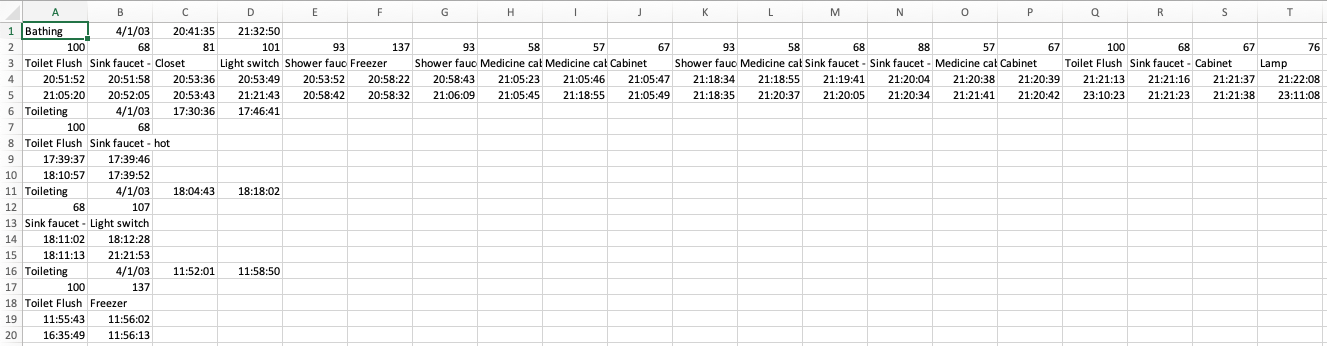
\includegraphics[width=1\linewidth]{/Users/alistairgj/Documents/GitHub/IoT_ResearchProject/IoT_November/images/s1actExcel} 

}

\caption{The S1 Activities dataset shown in a spreadsheet program. The structure of the data, a mixture of tab delimited and comma delimited values with unequal row lengths, presents a variety of challenges with respect to pre-processing}\label{fig:s1actExcel}
\end{figure}

\rowcolors{2}{gray!6}{white}
\begin{table}[!h]

\caption{\label{tab:TAB_rawDSS1}A sample of the S1 activities dataset after importation into the interactive development environment}
\centering
\fontsize{8}{10}\selectfont
\begin{tabular}[t]{ll}
\hiderowcolors
\toprule
  & 0\\
\midrule
\showrowcolors
5 & Toileting,4/1/2003,17:30:36,17:46:41\\
6 & 100,68\\
7 & Toilet Flush,Sink faucet - hot\\
8 & 17:39:37,17:39:46\\
9 & 18:10:57,17:39:52\\
\bottomrule
\end{tabular}
\end{table}
\rowcolors{2}{white}{white}

Due to the varying number of comma-separated elements in each row
(Figure \ref{fig:s1actExcel}) the \texttt{S1activities.csv} data was
imported as an indexed dataframe, containing only one column, with 1475
rows. In each row, values were comma-separated. After initial imporation
the dataframe was converted to a 2D array, using \texttt{np.array()},
where each row from the dataframe became an array within the 2D array.
The 2D array was flattened to a 1D array using \texttt{.flatten()} and
each group of observations was then chunked into a list of 5. Using the
logic shown in Algorithm \ref{alg:actExtraction}, below, the activity,
date and time data was extracted. During extraction in intermediate
activities dataset was generated as seen below in Table
\ref{tab:TAB_dsActIntermediate} followed by the tidy pre-processed
activities dataset, as seen in Table \ref{tab:TAB_dsActFinal}.

\begin{algorithm}[H]
\DontPrintSemicolon
\SetAlgoLined
\KwResult{Intermediate dataframe with 'activity', 'date', 'startTime', 'endTime' as attributes}
\SetKwInOut{Input}{Input}\SetKwInOut{Output}{Output}
\Input{S1 Activities}
\Output{S1 Activities Intermediate}
\BlankLine
\Begin{
  array1-8 = [ ]\;
  i = 0\;
  \While{i < length(dataframe)}{
    array1.append(dataframe[i][0])\;
    array2.append([x.strip() for x in array1[i].split(',')])\;
    array3.append(array2[i][0])\;
    array4.append(array2[i][1])\;
    array5.append(array2[i][2])\;
    array6.append(array2[i][3])\;
    i = i + 1\;
    }
  dfIntermediate = pandas.DataFrame(list(zip(array3, array4, array5, array6)))\;
  start = (dfIntermediate.date + " " + dfIntermediate.startTime)\;
  end = (dfIntermediate.date + " " + dfIntermediate.endTime)\;
  i = 0\;
  \While{i < length(start)}{
    array7.append(datetime.strptime(start[i], mm/dd/yyyy HH:MM:SS))\;
    array8.append(datetime.strptime(end[i], mm/dd/yyyy HH:MM:SS))\;
    i = i + 1\;
    }
  dfFinal = pandas.DataFrame(list(zip(array3, array7, array8)))\;
  \KwRet dfIntermediate\;
  \KwRet dfFinal\;
}
\caption{Extraction of data from S1 Activities dataset}
\label{alg:actExtraction}
\end{algorithm}

\rowcolors{2}{gray!6}{white}
\begin{table}[!h]

\caption{\label{tab:TAB_dsActIntermediate}The S1 Activities intermediate dataset}
\centering
\fontsize{8}{10}\selectfont
\begin{tabular}[t]{llll}
\hiderowcolors
\toprule
activity & date & startTime & endTime\\
\midrule
\showrowcolors
Bathing & 4/1/2003 & 20:41:35 & 21:32:50\\
Toileting & 4/1/2003 & 17:30:36 & 17:46:41\\
Toileting & 4/1/2003 & 18:4:43 & 18:18:2\\
Toileting & 4/1/2003 & 11:52:1 & 11:58:50\\
Going out to work & 4/1/2003 & 12:11:26 & 12:15:12\\
\addlinespace
Preparing lunch & 4/1/2003 & 11:21:17 & 11:38:22\\
\bottomrule
\end{tabular}
\end{table}
\rowcolors{2}{white}{white}

\rowcolors{2}{gray!6}{white}
\begin{table}[!h]

\caption{\label{tab:TAB_dsActFinal}The S1 activities tidy dataset}
\centering
\fontsize{8}{10}\selectfont
\begin{tabular}[t]{lll}
\hiderowcolors
\toprule
activity & start & end\\
\midrule
\showrowcolors
Bathing & 2003-04-01 20:41:35 & 2003-04-01 21:32:50\\
Toileting & 2003-04-01 17:30:36 & 2003-04-01 17:46:41\\
Toileting & 2003-04-01 18:04:43 & 2003-04-01 18:18:02\\
Toileting & 2003-04-01 11:52:01 & 2003-04-01 11:58:50\\
Going out to work & 2003-04-01 12:11:26 & 2003-04-01 12:15:12\\
\addlinespace
Preparing lunch & 2003-04-01 11:21:17 & 2003-04-01 11:38:22\\
\bottomrule
\end{tabular}
\end{table}
\rowcolors{2}{white}{white}

\hypertarget{importing-visualizing-and-preprocessing-the-subactivities-data}{%
\subsection{Importing, Visualizing and Preprocessing the SubActivities
Data}\label{importing-visualizing-and-preprocessing-the-subactivities-data}}

As mentioned above, the \texttt{S1Activities\_data.csv} dataset contains
the collated activity and subactivity data from the work of Rockinson
{[}\protect\hyperlink{ref-rockinsonActivityRecognitionHome}{20}{]}. As
with the activities data extraction, the dataframe was converted to a 2D
array, using \texttt{np.array()}, where each row from the dataframe
became an array within the 2D array. The 2D array was flattened to a 1D
array using \texttt{.flatten()} and each group of observations was then
chunked into a list of 5. The sub-activity, date and time data was then
extracted from the dataset, by employing the logic shown in Algorithm
\ref{alg:subActExtraction}, below.An intermediate sub-activities dataset
was generated as seen below in Table \ref{tab:TAB_dsSUBIntermediate}
followed by the tidy pre-processed sub-activities dataset, as seen in
Table \ref{tab:TAB_dsSUBActFinal}. This dataset was exported as
\texttt{S1SubActivities\_ds.csv}.

\begin{algorithm}[H]
\DontPrintSemicolon
\SetAlgoLined
\KwResult{Intermediate dataframe with 'activity', 'date', 'startTime', 'endTime' as attributes}
\SetKwInOut{Input}{Input}\SetKwInOut{Output}{Output}
\Input{S1 Activities}
\Output{S1 Activities Intermediate}
\BlankLine
\Begin{
  array1-21 = [ ]\;
  
  \While{i < length(dataframe)}{
    array1.append(dataframe[i][0])\;
    array2.append([x.strip() for x in array1[i].split(',')])\;
    array3.append(array2[i][0])\;
    array4.append(array2[i][1])\;
    array5.append(array2[i][2])\;
    array6.append(array2[i][3])\;
    i = i + 1\;
    }
  \While{i < length(dataframe)}{
    array7.append(dataframe[i][1])\;
    array8.append([x.strip() for x in array7[i].split(',')])\;
    array9.append(dataframe[i][2])\;
    array10.append([x.strip() for x in array9[i].split(',')])\;
    array11.append(dataframe[i][3])\;
    array12.append([x.strip() for x in array11[i].split(',')])\;
    array13.append(dataframe[i][4])\;
    array14.append([x.strip() for x in array13[i].split(',')])\;
    i = i + 1\;  
    }
  \While{i < length(dataframe)}{
    for x in range(len(array8[i])) : array15.append(array4[i])\;
    i = i + 1\;  
    }
  for sublist in array8: for item in sublist: array16.append(item)\;
  for sublist in array10: for item in sublist: array17.append(item)\;
  for sublist in array12: for item in sublist: array18.append(item)\;
  for sublist in array13: for item in sublist: array19.append(item)\;
  dfIntermediate = pandas.DataFrame(list(zip(array16, array17, array15, array18, array19)))\;
  start = (dfIntermediate.date + " " + dfIntermediate.startTime)\;
  end = (dfIntermediate.date + " " + dfIntermediate.endTime)\;
  \While{i < length(start)}{
    array20.append(datetime.strptime(start[i], mm/dd/yyyy HH:MM:SS))\;
    array21.append(datetime.strptime(end[i], mm/dd/yyyy HH:MM:SS))\;
    i = i + 1\;
    }
  dfFinal = pandas.DataFrame(list(zip(array16, array17, array20, array21)))\;
  \KwRet dfIntermediate\;
  \KwRet dfFinal\;
}
\caption{Extraction of sub-activity data from S1 activities dataset}
\label{alg:subActExtraction}
\end{algorithm}

\pagebreak

\rowcolors{2}{gray!6}{white}
\begin{table}[!h]

\caption{\label{tab:TAB_dsSUBIntermediate}The S1 sub-activities intermediate dataset}
\centering
\fontsize{8}{10}\selectfont
\begin{tabular}[t]{rllll}
\hiderowcolors
\toprule
subActNum & subAct & date & startTime & endTime\\
\midrule
\showrowcolors
100 & Toilet Flush & 4/1/2003 & 20:51:52 & 21:5:20\\
68 & Sink faucet - hot & 4/1/2003 & 20:51:58 & 20:52:5\\
81 & Closet & 4/1/2003 & 20:53:36 & 20:53:43\\
101 & Light switch & 4/1/2003 & 20:53:49 & 21:21:43\\
93 & Shower faucet & 4/1/2003 & 20:53:52 & 20:58:42\\
\addlinespace
137 & Freezer & 4/1/2003 & 20:58:22 & 20:58:32\\
\bottomrule
\end{tabular}
\end{table}
\rowcolors{2}{white}{white}
\rowcolors{2}{gray!6}{white}
\begin{table}[!h]

\caption{\label{tab:TAB_dsSUBActFinal}The S1 sub-activities tidy dataset}
\centering
\fontsize{8}{10}\selectfont
\begin{tabular}[t]{rlll}
\hiderowcolors
\toprule
subActNum & subAct & start & end\\
\midrule
\showrowcolors
67 & Cabinet & 2003-03-27 06:43:40 & 2003-03-27 06:43:43\\
100 & Toilet Flush & 2003-03-27 06:44:06 & 2003-03-27 07:12:41\\
101 & Light switch & 2003-03-27 06:44:20 & 2003-03-27 07:46:34\\
57 & Medicine cabinet & 2003-03-27 06:44:35 & 2003-03-27 06:44:48\\
58 & Medicine cabinet & 2003-03-27 06:44:36 & 2003-03-27 06:44:48\\
\addlinespace
67 & Cabinet & 2003-03-27 06:44:49 & 2003-03-27 06:44:56\\
\bottomrule
\end{tabular}
\end{table}
\rowcolors{2}{white}{white}

\hypertarget{amalgamating-duplicate-sub-activity-instances}{%
\subsubsection{Amalgamating `duplicate' sub-activity
instances}\label{amalgamating-duplicate-sub-activity-instances}}

As mentioned in \emph{Importing \& Preprocessing the Sensor Meta Data},
10 of the sensors have duplicated values, owing to the presence of more
than one sensor for certain activities. The sub-activity
\texttt{kitchen\_refrigerator}, for example, has the numbers {[}91, 126,
144{]} associated with it, as seen in Table \ref{tab:TAB_fridge}, below.
These values are subsequently replaced with {[}126{]}. As is the case
with all sub-activities with degenerate numbers, the end value is chosen
based on the first appearance in the S1 Sensors dataset.

All duplicated values, as seen in Table \ref{tab:TAB_numDupes} were
aggregated to have the same sensor ID / subAct number, thus giving a
value of n=1 with respect to duplication.The first occurence of each
degenerate subactivity provided the subAct number to be used for all
subsequent instances. This dataset was exported as
\texttt{S1SubActivities\_preprocessed.csv}. **It was found these data
has dimensionality of \_\_\_**

\rowcolors{2}{gray!6}{white}
\begin{table}[!h]

\caption{\label{tab:TAB_fridge}Example of duplicate sub-activity number removal}
\centering
\resizebox{\linewidth}{!}{\fontsize{8}{10}\selectfont
\begin{tabular}[t]{rlllrlll}
\hiderowcolors
\toprule
\multicolumn{4}{c}{Prior to duplicate removal} & \multicolumn{4}{c}{Post to duplicate removal} \\
\cmidrule(l{2pt}r{2pt}){1-4} \cmidrule(l{2pt}r{2pt}){5-8}
subActNum\_pr & subAct\_pr & start\_pr & end\_pr & subActNum\_po & subAct\_po & start\_po & end\_po\\
\midrule
\showrowcolors
91 & kitchen\_refrigerator & 27/3/03 7:41 & 27/3/03 7:41 & 126 & kitchen\_refrigerator & 27/3/03 7:41 & 27/3/03 7:41\\
91 & kitchen\_refrigerator & 27/3/03 11:38 & 27/3/03 11:38 & 126 & kitchen\_refrigerator & 27/3/03 11:38 & 27/3/03 11:38\\
126 & kitchen\_refrigerator & 29/3/03 14:42 & 29/3/03 14:42 & 126 & kitchen\_refrigerator & 29/3/03 14:42 & 29/3/03 14:42\\
144 & kitchen\_refrigerator & 29/3/03 14:42 & 29/3/03 14:42 & 126 & kitchen\_refrigerator & 29/3/03 14:42 & 29/3/03 14:42\\
126 & kitchen\_refrigerator & 29/3/03 14:43 & 29/3/03 14:43 & 126 & kitchen\_refrigerator & 29/3/03 14:43 & 29/3/03 14:43\\
\bottomrule
\end{tabular}}
\end{table}
\rowcolors{2}{white}{white}

\hypertarget{addition-of-temporal-features-to-the-pre-processed-sub-activities-data}{%
\subsubsection{Addition of Temporal Features to the pre-processed
sub-activities
data}\label{addition-of-temporal-features-to-the-pre-processed-sub-activities-data}}

As noted by Basu et al, human behavior with respect to home appliance
interaction and activity, is typically periodic in nature
{[}\protect\hyperlink{ref-kaustavbasuApplianceUsagePrediction2012}{18}{]},
that is, certain activities occur at specific times of day or in a
particular sequence. It is helpful therefore to add categorical temporal
features to our dataset, in order to inform further analysis. Using the
Python \texttt{pandas} and \texttt{datetime} packages, the following
features were added to all instances of the pre-processed S1 sub
activities dataset; \texttt{dayNumeric}, \texttt{DAY}, \texttt{WDWE}
(where WD is weekday and WE is weekend), \texttt{HOUR} (based on 24-hour
time) and \texttt{durationSec} (the delta seconds value between
\texttt{start} and \texttt{end}). This dataset was exported as
\texttt{S1SubActivities\_preprocessedWfeatures.csv}.

\rowcolors{2}{gray!6}{white}
\begin{table}[!h]

\caption{\label{tab:TAB_}A sample of n=1 of each sub-activity from the pre-processed dataset. The table has been coloured to indicate futher pre-processing steps, as discussed below.}
\centering
\resizebox{\linewidth}{!}{\fontsize{8}{10}\selectfont
\begin{tabular}[t]{>{}l>{}lllllllr}
\hiderowcolors
\toprule
subActNum & subAct & start & end & dayNumeric & DAY & WDWE & HOUR & durationSec\\
\midrule
\showrowcolors
\rowcolor[HTML]{C6CDF2}  67 & bathroom\_cabinet & 2003-03-27 06:43:40 & 2003-03-27 06:43:43 & 3 & Thu & WD & 6 & 4\\
\rowcolor[HTML]{FAF8B9}  100 & bathroom\_toiletflush & 2003-03-27 06:44:06 & 2003-03-27 07:12:41 & 3 & Thu & WD & 6 & 1716\\
\rowcolor[HTML]{EACBF2}  101 & bathroom\_lightswitch & 2003-03-27 06:44:20 & 2003-03-27 07:46:34 & 3 & Thu & WD & 6 & 3735\\
\rowcolor[HTML]{C6CDF2}  57 & bathroom\_medicinecabinet & 2003-03-27 06:44:35 & 2003-03-27 06:44:48 & 3 & Thu & WD & 6 & 14\\
\rowcolor[HTML]{C6CDF2}  82 & study\_drawer & 2003-03-27 06:45:45 & 2003-03-27 06:45:48 & 3 & Thu & WD & 6 & 4\\
\addlinespace
\rowcolor[HTML]{C6CDF2}  146 & bedroom\_drawer & 2003-03-27 06:46:12 & 2003-03-27 06:46:20 & 3 & Thu & WD & 6 & 9\\
\rowcolor[HTML]{C6CDF2}  132 & kitchen\_cabinet & 2003-03-27 06:51:43 & 2003-03-27 06:51:46 & 3 & Thu & WD & 6 & 4\\
\rowcolor[HTML]{C6CDF2}  143 & kitchen\_microwave & 2003-03-27 06:54:09 & 2003-03-27 13:07:43 & 3 & Thu & WD & 6 & 22415\\
\rowcolor[HTML]{C6CDF2}  141 & kitchen\_door & 2003-03-27 06:57:05 & 2003-03-27 06:57:08 & 3 & Thu & WD & 6 & 4\\
\rowcolor[HTML]{C6CDF2}  93 & bathroom\_showerfaucet & 2003-03-27 07:05:22 & 2003-03-27 07:05:24 & 3 & Thu & WD & 7 & 3\\
\addlinespace
\rowcolor[HTML]{C6CDF2}  125 & kitchen\_drawer & 2003-03-27 07:38:48 & 2003-03-27 07:38:51 & 3 & Thu & WD & 7 & 4\\
\rowcolor[HTML]{C6CDF2}  70 & kitchen\_dishwasher & 2003-03-27 07:40:32 & 2003-03-27 07:40:34 & 3 & Thu & WD & 7 & 3\\
\rowcolor[HTML]{EACBF2}  126 & kitchen\_refrigerator & 2003-03-27 07:41:08 & 2003-03-27 07:41:16 & 3 & Thu & WD & 7 & 9\\
\rowcolor[HTML]{EACBF2}  88 & bathroom\_sinkfaucet-cold & 2003-03-27 07:43:22 & 2003-03-27 07:43:48 & 3 & Thu & WD & 7 & 27\\
\rowcolor[HTML]{C6CDF2}  68 & bathroom\_sinkfaucet-hot & 2003-03-27 07:43:23 & 2003-03-27 07:43:48 & 3 & Thu & WD & 7 & 26\\
\addlinespace
\rowcolor[HTML]{EACBF2}  140 & foyer\_door & 2003-03-27 07:48:49 & 2003-03-27 07:48:53 & 3 & Thu & WD & 7 & 5\\
\rowcolor[HTML]{C6CDF2}  137 & kitchen\_freezer & 2003-03-27 11:36:15 & 2003-03-27 11:36:21 & 3 & Thu & WD & 11 & 7\\
\rowcolor[HTML]{EACBF2}  106 & kitchen\_burner & 2003-03-27 11:37:13 & 2003-03-27 11:42:24 & 3 & Thu & WD & 11 & 312\\
\rowcolor[HTML]{C6CDF2}  105 & kitchen\_lightswitch & 2003-03-27 11:38:54 & 2003-03-27 12:31:05 & 3 & Thu & WD & 11 & 3132\\
\rowcolor[HTML]{C6CDF2}  92 & study\_lightwitch & 2003-03-27 16:28:23 & 2003-03-27 18:44:14 & 3 & Thu & WD & 16 & 8152\\
\addlinespace
\rowcolor[HTML]{C6CDF2}  130 & bathroom\_door & 2003-03-27 17:43:10 & 2003-03-27 17:43:12 & 3 & Thu & WD & 17 & 3\\
\rowcolor[HTML]{EACBF2}  104 & foyer\_lightswitch & 2003-03-27 19:36:32 & 2003-03-27 19:50:07 & 3 & Thu & WD & 19 & 816\\
\rowcolor[HTML]{C6CDF2}  131 & kitchen\_toaster & 2003-03-28 12:32:00 & 2003-03-28 15:10:16 & 4 & Fri & WD & 12 & 9497\\
\rowcolor[HTML]{EACBF2}  96 & bathroom\_exhaustfan & 2003-03-28 17:43:17 & 2003-03-28 18:25:19 & 4 & Fri & WD & 17 & 2523\\
\rowcolor[HTML]{EACBF2}  108 & bedroom\_lightswitch & 2003-03-28 18:24:48 & 2003-03-28 19:55:44 & 4 & Fri & WD & 18 & 5457\\
\addlinespace
\rowcolor[HTML]{EACBF2}  129 & kitchen\_oven & 2003-03-28 19:09:26 & 2003-03-28 19:09:30 & 4 & Fri & WD & 19 & 5\\
\rowcolor[HTML]{CEF5E7}  56 & livingroom\_dvd & 2003-03-28 19:55:24 & 2003-03-28 19:55:29 & 4 & Fri & WD & 19 & 6\\
\rowcolor[HTML]{EACBF2}  76 & livingroom\_lamp & 2003-03-29 13:30:51 & 2003-03-29 18:50:13 & 5 & Sat & WE & 13 & 19163\\
\rowcolor[HTML]{CEF5E7}  139 & bedroom\_jewelrybox & 2003-03-29 15:12:44 & 2003-03-29 15:12:45 & 5 & Sat & WE & 15 & 2\\
\rowcolor[HTML]{EACBF2}  142 & kitchen\_washingmachine & 2003-03-29 15:44:24 & 2003-03-29 15:44:26 & 5 & Sat & WE & 15 & 3\\
\addlinespace
\rowcolor[HTML]{EACBF2}  90 & kitchen\_laundrydryer & 2003-03-29 15:48:18 & 2003-03-29 15:48:54 & 5 & Sat & WE & 15 & 37\\
\rowcolor[HTML]{EACBF2}  98 & kitchen\_garbagedisposal & 2003-03-29 15:54:50 & 2003-03-29 15:54:51 & 5 & Sat & WE & 15 & 2\\
\rowcolor[HTML]{C6CDF2}  107 & livingroom\_lightswitch & 2003-03-29 18:50:43 & 2003-03-29 18:51:09 & 5 & Sat & WE & 18 & 27\\
\rowcolor[HTML]{CEF5E7}  81 & foyer\_closet & 2003-04-01 06:13:26 & 2003-04-01 06:13:34 & 1 & Tue & WD & 6 & 9\\
\rowcolor[HTML]{CEF5E7}  145 & kitchen\_cereal & 2003-04-01 06:37:18 & 2003-04-01 06:37:59 & 1 & Tue & WD & 6 & 42\\
\addlinespace
\rowcolor[HTML]{CEF5E7}  60 & kitchen\_containers & 2003-04-01 06:38:14 & 2003-04-01 06:38:48 & 1 & Tue & WD & 6 & 35\\
\rowcolor[HTML]{EACBF2}  119 & kitchen\_coffeemachine & 2003-04-09 08:46:07 & 2003-04-09 08:46:35 & 2 & Wed & WD & 8 & 29\\
\rowcolor[HTML]{CEF5E7}  64 & bedroom\_lamp & 2003-04-09 20:16:36 & 2003-04-09 21:13:19 & 2 & Wed & WD & 20 & 3404\\
\bottomrule
\end{tabular}}
\end{table}
\rowcolors{2}{white}{white}

\pagebreak

\hypertarget{subactivity-visualisation-and-outlier-inspection}{%
\subsubsection{SubActivity Visualisation and Outlier
Inspection}\label{subactivity-visualisation-and-outlier-inspection}}

\hypertarget{aggregated-line-chart}{%
\paragraph{Aggregated Line Chart}\label{aggregated-line-chart}}

The \texttt{S1SubActivities\_preprocessedWfeatures.csv} dataset was
analysed using data visualisation techniques. A plot of aggregated
sub-activity count versus sub-activity was generated, as seen in Figure
\ref{fig:FIG_aggLineChart}, below. The chart shows that there is a high
level of consistency with respect to the overall aggregated count of
each sub-activity, when compared to the feature
\texttt{Day\ of\ the\ Week}. \textbf{This is helpful for subsequent
analysis.}

\begin{figure}[H]

{\centering 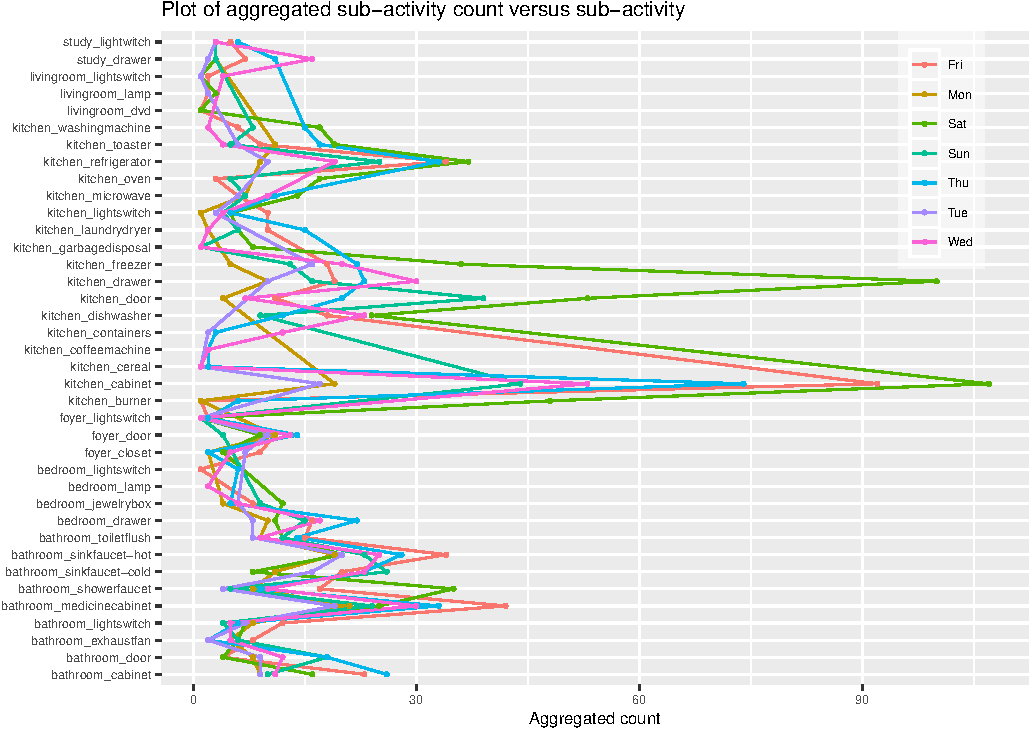
\includegraphics{MD_Final_files/figure-latex/FIG_aggLineChart-1} 

}

\caption{ADD Text}\label{fig:FIG_aggLineChart}
\end{figure}

\pagebreak

\hypertarget{aggregated-box-plot-of-sub-activities}{%
\paragraph{Aggregated Box Plot of
Sub-Activities}\label{aggregated-box-plot-of-sub-activities}}

Figure \ref{fig:FIG_allBoxPlots}, below, shows boxplots of all
sub-activities versus their duration values. In this plot, we can see
many outliers, which will inform further analysis. We also note that
many of the outliers are extremely unrealistic. Of particular concern
Kitchen\_Toaster with a duration of almost 30,000 seconds,
Bathroom\_toiletflush distributed up to the range of 20,000 seconds.
This potentially indicates challenges with the initial data collection
methodology or experimental conditions / setup. Each sub-activity will
be individually considered with respect to it's outliers.

\begin{figure}[H]

{\centering 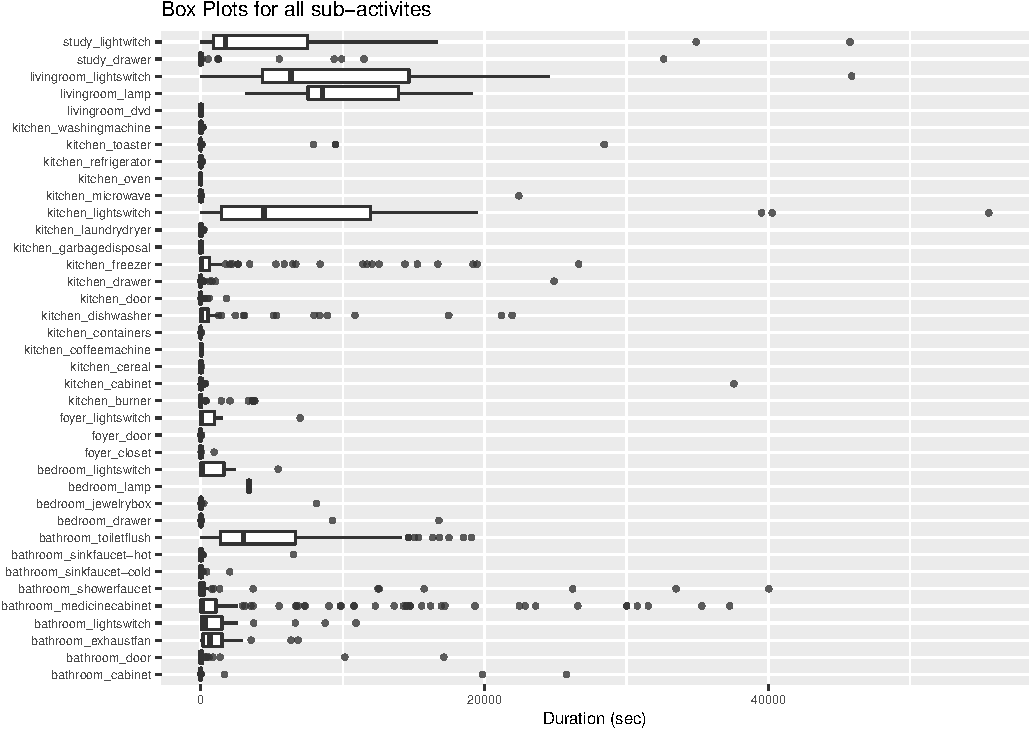
\includegraphics{MD_Final_files/figure-latex/FIG_allBoxPlots-1} 

}

\caption{ADD Text}\label{fig:FIG_allBoxPlots}
\end{figure}

\pagebreak

\hypertarget{sub-activity-cleansing---outlier-removal}{%
\subsubsection{Sub-Activity Cleansing - Outlier
Removal}\label{sub-activity-cleansing---outlier-removal}}

Via the inspection of each sub-activity the following set of instances
were identified, as seen in Table \ref{tab:outlierSTATS}. In all cases
the standard deviation (\textbf{Std}) of each aggregated instance
(n=Count) is found to be greater than the mean, indicating **\_\_\_**.
THe bathroom medicine cabinet, for example, has a mean value of 3188
seconds (53 minutes) and a median value of 88 seconds. Accross all
sub-activities seen in Table \ref{tab:outlierSTATS}, the median gives
more reasonable values. Therefore the median will be used to fill the
outlier values.

\begin{Shaded}
\begin{Highlighting}[]
\CommentTok{# cleanseOutliers.py}
\ControlFlowTok{for}\NormalTok{ row }\KeywordTok{in}\NormalTok{ allMedianValues.iterrows():}
\NormalTok{    ds.loc[(ds[}\StringTok{'subAct'}\NormalTok{] }\OperatorTok{==}\NormalTok{ row[}\DecValTok{1}\NormalTok{].SubAct) }\OperatorTok{&}
\NormalTok{           (ds[}\StringTok{'durationSec'}\NormalTok{] }\OperatorTok{>}\NormalTok{ row[}\DecValTok{1}\NormalTok{].Median }\OperatorTok{+} \FloatTok{0.5} \OperatorTok{*}\NormalTok{ row[}\DecValTok{1}\NormalTok{].Std),}
           \StringTok{'durationSec'}\NormalTok{] }\OperatorTok{=} \BuiltInTok{round}\NormalTok{(row[}\DecValTok{1}\NormalTok{].Median)}

\ImportTok{from}\NormalTok{ datetime }\ImportTok{import}\NormalTok{ datetime, timedelta}
\NormalTok{ds.end }\OperatorTok{=}\NormalTok{ ds.}\BuiltInTok{apply}\NormalTok{(}\KeywordTok{lambda}\NormalTok{ x: x.start }\OperatorTok{+}\NormalTok{ timedelta(seconds}\OperatorTok{=}\NormalTok{x.durationSec), axis}\OperatorTok{=}\DecValTok{1}\NormalTok{)}
\end{Highlighting}
\end{Shaded}

\rowcolors{2}{gray!6}{white}
\begin{table}[!h]

\caption{\label{tab:outlierSTATS}Demo table}
\centering
\fontsize{8}{10}\selectfont
\begin{tabular}[t]{lrrrr}
\hiderowcolors
\toprule
SubAct & Count & Median & Mean & Std\\
\midrule
\showrowcolors
bathroom\_cabinet & 104 & 4.0 & 460.22115 & 3176.1633\\
bathroom\_medicinecabinet & 194 & 88.0 & 3188.97423 & 7354.1424\\
study\_drawer & 45 & 6.0 & 1634.48889 & 5432.4063\\
bedroom\_drawer & 99 & 10.0 & 273.47475 & 1918.7262\\
kitchen\_cabinet & 406 & 7.0 & 112.82020 & 1864.0122\\
\addlinespace
kitchen\_microwave & 61 & 6.0 & 377.40984 & 2868.6679\\
kitchen\_door & 134 & 4.0 & 46.11194 & 174.1857\\
bathroom\_showerfaucet & 88 & 15.0 & 1754.35227 & 6540.7295\\
kitchen\_drawer & 208 & 4.0 & 145.06250 & 1727.5767\\
bathroom\_sinkfaucet-hot & 169 & 11.0 & 57.90533 & 501.2729\\
\addlinespace
kitchen\_freezer & 130 & 39.0 & 1738.10769 & 4512.5738\\
bathroom\_door & 73 & 17.0 & 461.61644 & 2310.8116\\
kitchen\_toaster & 71 & 5.0 & 790.36620 & 3793.6744\\
kitchen\_lightswitch & 32 & 4454.0 & 9318.71875 & 13081.3404\\
study\_lightwitch & 26 & 1728.5 & 6430.73077 & 11002.3025\\
\addlinespace
kitchen\_dishwasher & 86 & 63.5 & 1518.40698 & 4146.6375\\
livingroom\_lightswitch & 8 & 6352.5 & 12545.12500 & 15556.6628\\
foyer\_closet & 29 & 8.0 & 42.44828 & 174.4286\\
\bottomrule
\end{tabular}
\end{table}
\rowcolors{2}{white}{white}

There were in total 4 pre-processing methodologies used. 1. Filling
outliers with median 2. All values replaced with one value 3. No futher
processing required 3. Sub-activity dropped

\hypertarget{sub-activity-cleansing---1-filling-outliers-with-median}{%
\subsubsection{Sub-Activity Cleansing - 1) Filling outliers with
median}\label{sub-activity-cleansing---1-filling-outliers-with-median}}

This methodology is exemplified by the bathroom cabinet. This was also
applied to

\hypertarget{bathroom-cabinet}{%
\paragraph{Bathroom Cabinet}\label{bathroom-cabinet}}

\begin{figure}[H]

{\centering 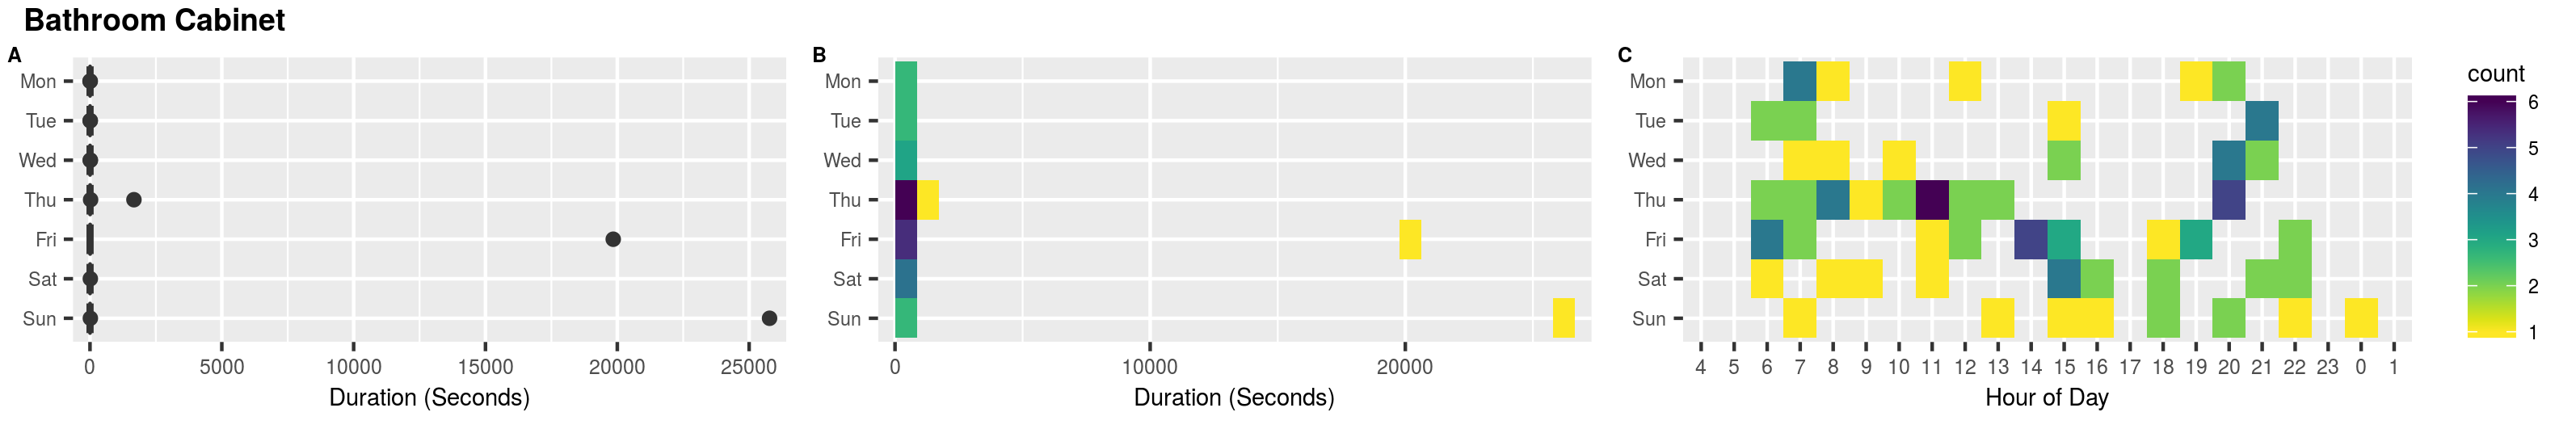
\includegraphics[width=1\linewidth]{/Users/alistairgj/Documents/GitHub/IoT_ResearchProject/IoT_November/images/subAct67} 

}

\caption{A caption}\label{fig:subAct67}
\end{figure}

\hypertarget{subactivity-cleansing---2-all-values-replaced-with-one-value}{%
\subsubsection{SubActivity Cleansing - 2) All values replaced with one
value}\label{subactivity-cleansing---2-all-values-replaced-with-one-value}}

This methodology was applied only to the bathroom toiletflush, with all
values being set to 1 second.

\hypertarget{bathroom-toiletflush}{%
\paragraph{Bathroom Toiletflush}\label{bathroom-toiletflush}}

\begin{figure}[H]

{\centering 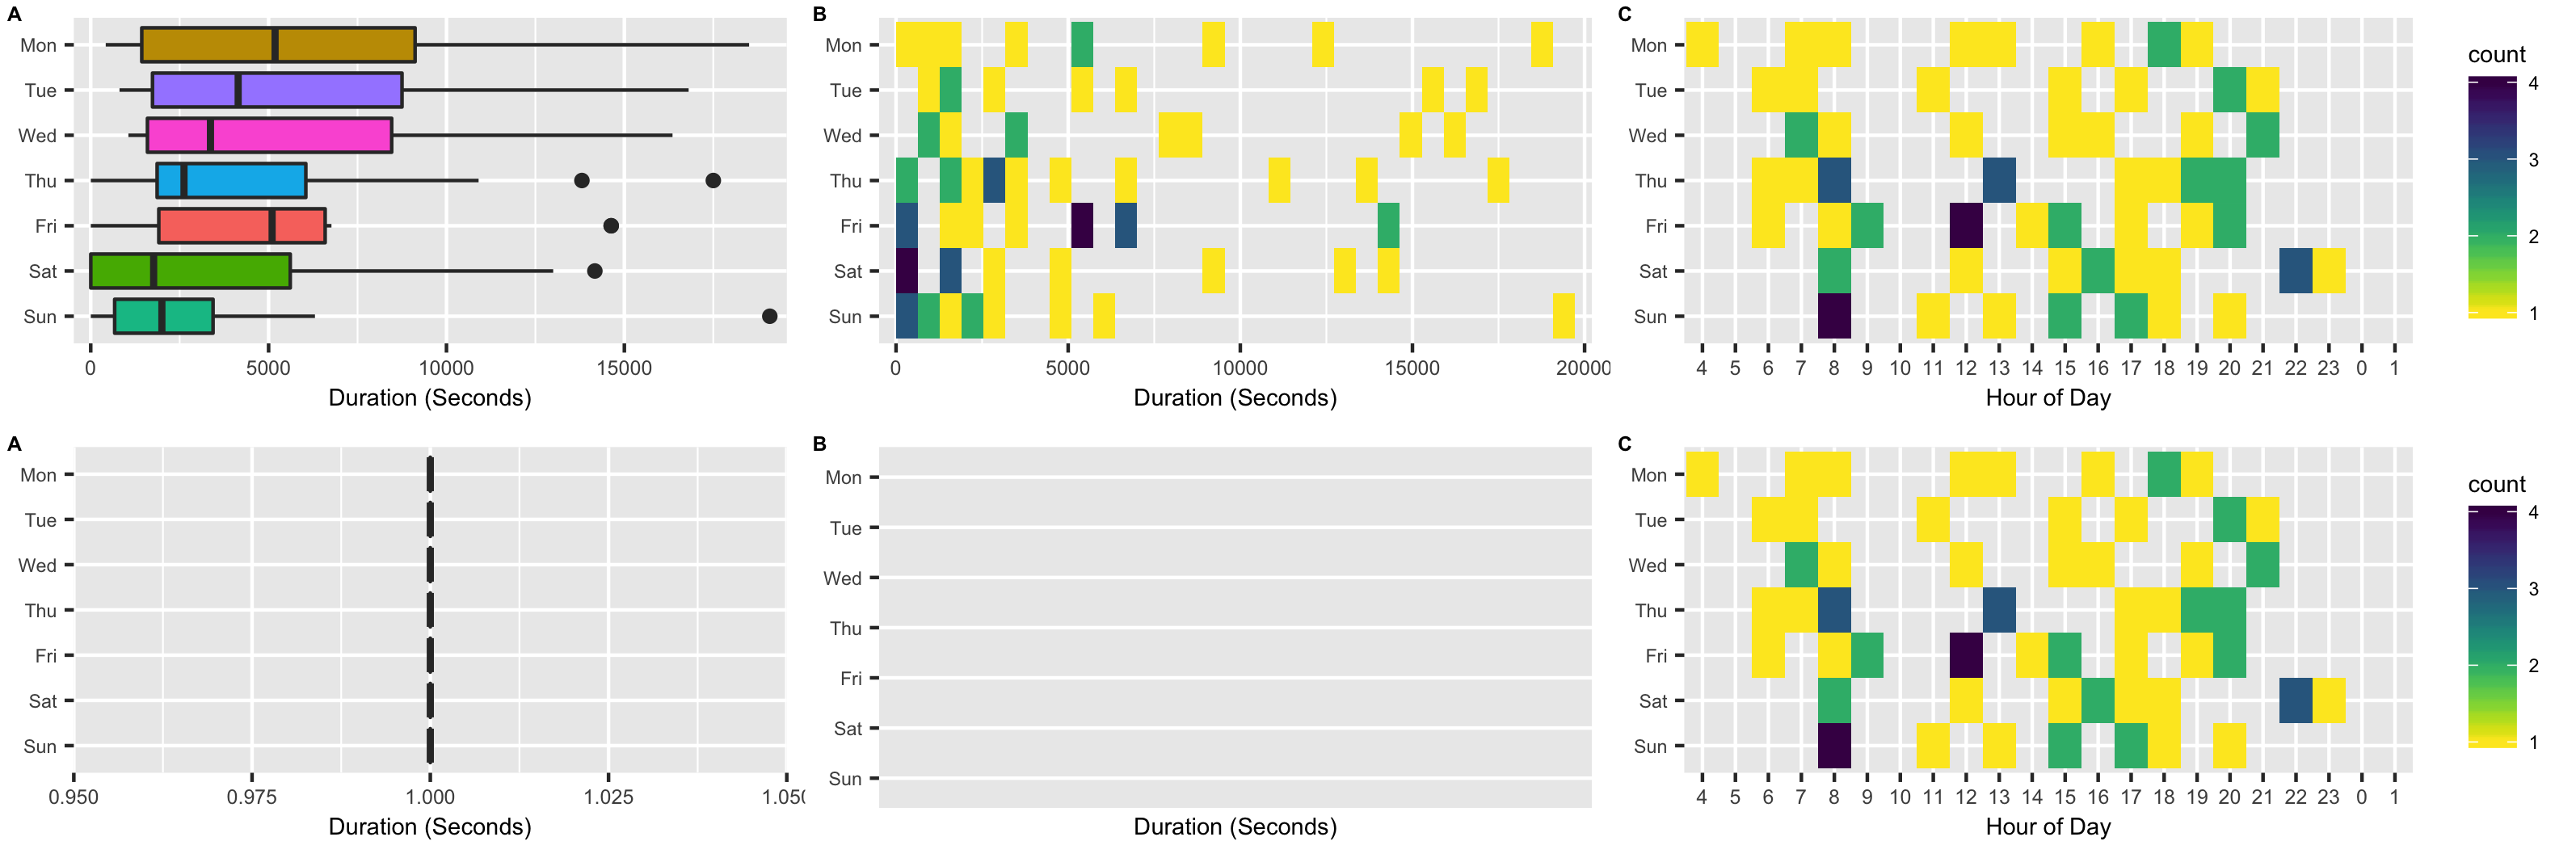
\includegraphics[width=1\linewidth]{/Users/alistairgj/Documents/GitHub/IoT_ResearchProject/IoT_November/images/subAct100} 

}

\caption{A caption}\label{fig:subAct100}
\end{figure}

\hypertarget{subactivity-cleansing-review---3-no-futher-processing-required}{%
\subsubsection{SubActivity Cleansing Review - 3) No futher processing
required}\label{subactivity-cleansing-review---3-no-futher-processing-required}}

Based on the investigation of the box plots (A in all sub activity
plots), heat maps of day of week versus duration in seconds mapped by
count (B in all subactivity plots) and heat maps of day of week versus
hour of day mapped by count (C in all subactivity plots) the following
sub activities were left in their native state;
\texttt{bathroom\_lightswitch}, \texttt{kitchen\_refrigerator},
\texttt{bathroom\_sinkfaucet-cold}, \texttt{foyer\_door},
\texttt{kitchen\_burner}, \texttt{foyer\_lightswitch},
\texttt{bathroom\_exhaustfan}, \texttt{bedroom\_lightswitch},
\texttt{kitchen\_oven}, \texttt{livingroom\_lamp},
\texttt{kitchen\_washingmachine}, \texttt{kitchen\_laundrydryer},
\texttt{kitchen\_garbagedisposal}, \texttt{kitchen\_coffeemachine},
\texttt{foyer\_closet} as seen highlighted \textbf{COLOUR} in .

\hypertarget{bathroom-lightswitch}{%
\paragraph{Bathroom Lightswitch}\label{bathroom-lightswitch}}

\begin{figure}[H]

{\centering 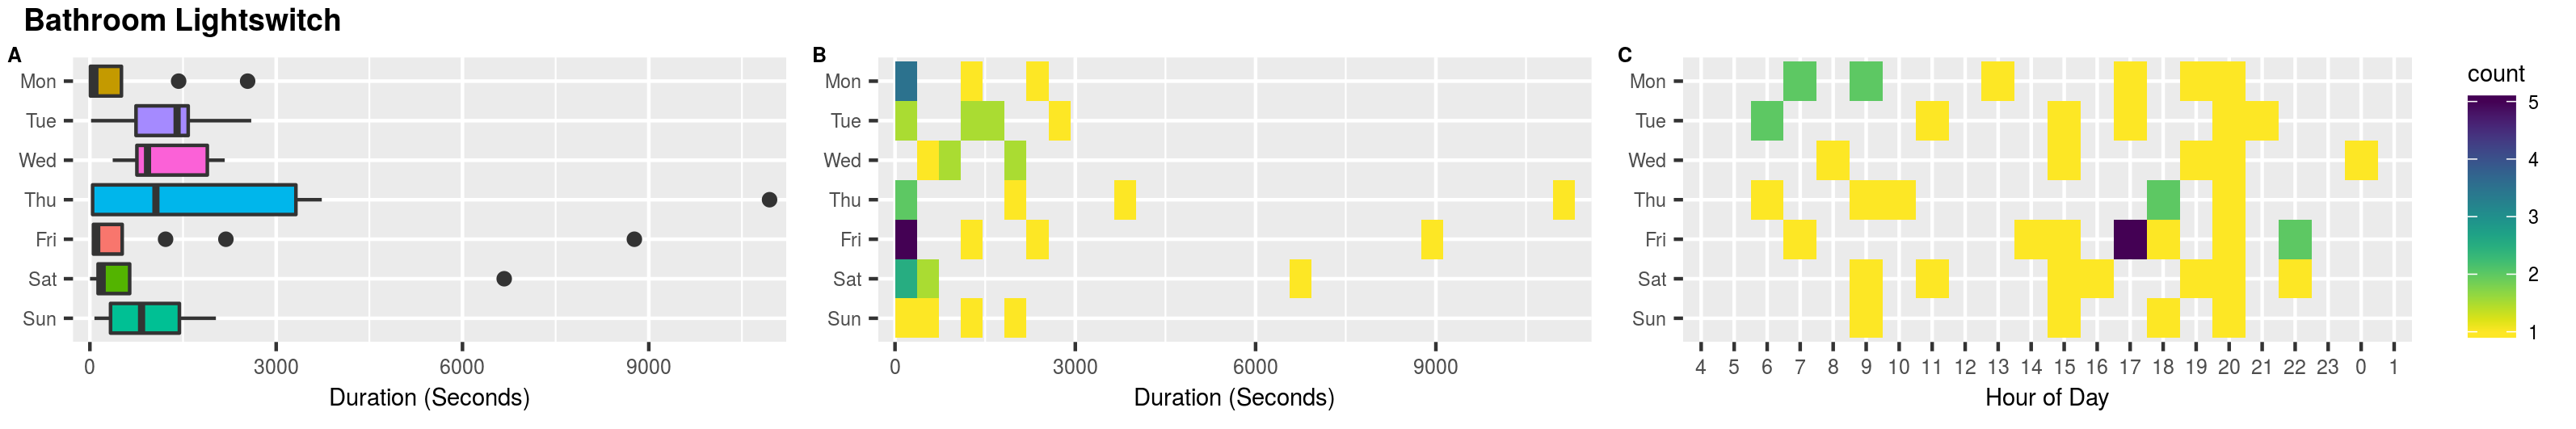
\includegraphics[width=1\linewidth]{/Users/alistairgj/Documents/GitHub/IoT_ResearchProject/IoT_November/images/subAct101} 

}

\caption{A caption}\label{fig:subAct101}
\end{figure}

\hypertarget{subactivity-cleansing---4-sub-activity-dropped}{%
\subsubsection{SubActivity Cleansing - 4) Sub-activity
dropped}\label{subactivity-cleansing---4-sub-activity-dropped}}

Based on the investigation of the box plots (A in all sub activity
plots), heat maps of day of week versus duration in seconds mapped by
count (B in all subactivity plots) and heat maps of day of week versus
hour of day mapped by count (C in all subactivity plots) the following
sub activities were dropped from the dataset.

\hypertarget{livingroom-dvd---subact56}{%
\paragraph{Livingroom DVD - SubAct56}\label{livingroom-dvd---subact56}}

This livingroom DVD sub activity, as plotted below in Figure
\ref{fig:subAct56} was dropped from the dataset due to it's sparsity
(only two instances in the dataset).

\begin{figure}[H]

{\centering 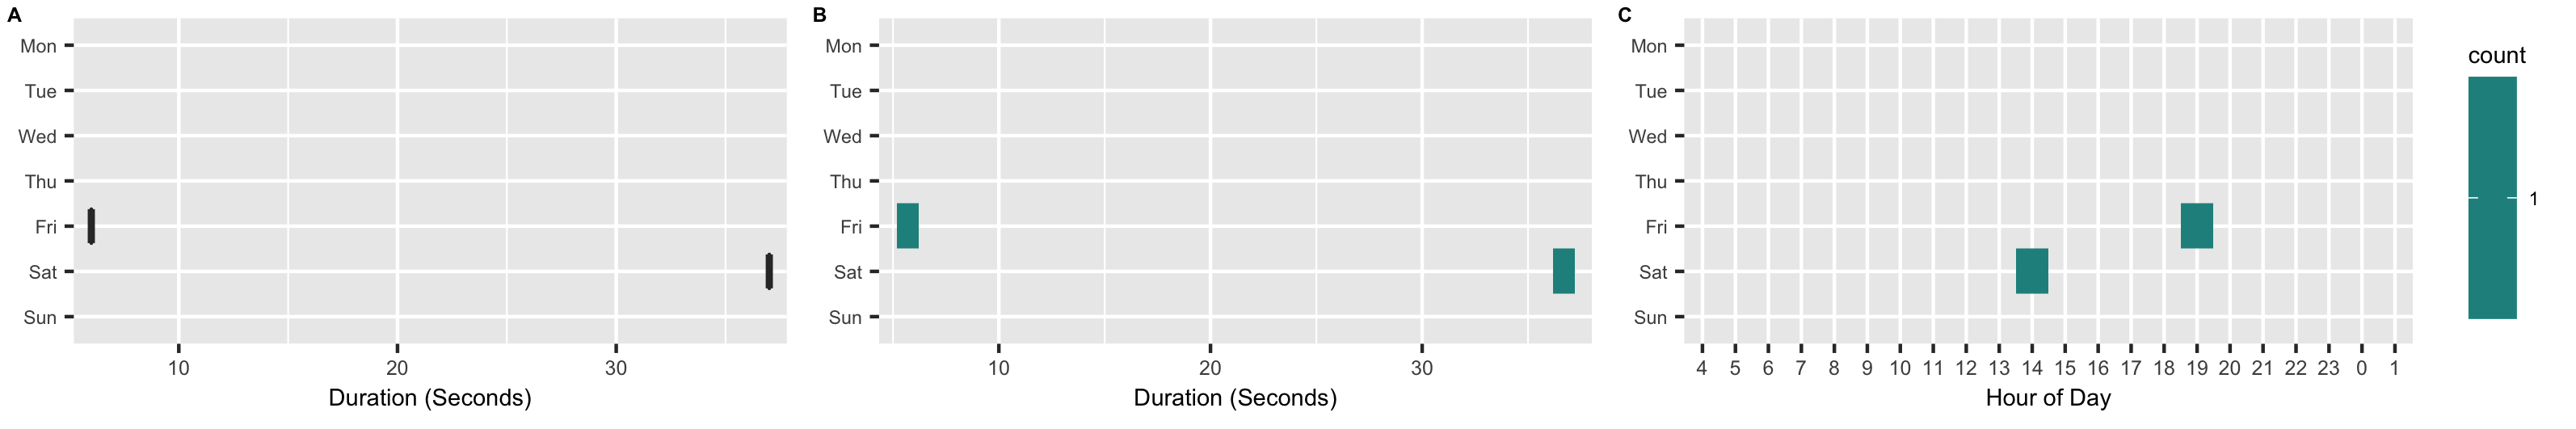
\includegraphics[width=1\linewidth]{/Users/alistairgj/Documents/GitHub/IoT_ResearchProject/IoT_November/images/subAct56} 

}

\caption{Box plot (A) and heat maps (B = day of week versus duration in seconds mapped by count, C = day of week versus hour of day mapped by count) for the Livingroom DVD sub activity.}\label{fig:subAct56}
\end{figure}

\hypertarget{bedroom-jewelrybox---subact139}{%
\paragraph{Bedroom Jewelrybox -
SubAct139}\label{bedroom-jewelrybox---subact139}}

The bedroom jewelrybox subactivity, as seen in Figure
\ref{fig:subAct139} was dropped due to the extremely specific nature of
this subactivity. In building a generalized model, we do not wish to
have such datapoints present for our analysis.

\begin{figure}[H]

{\centering 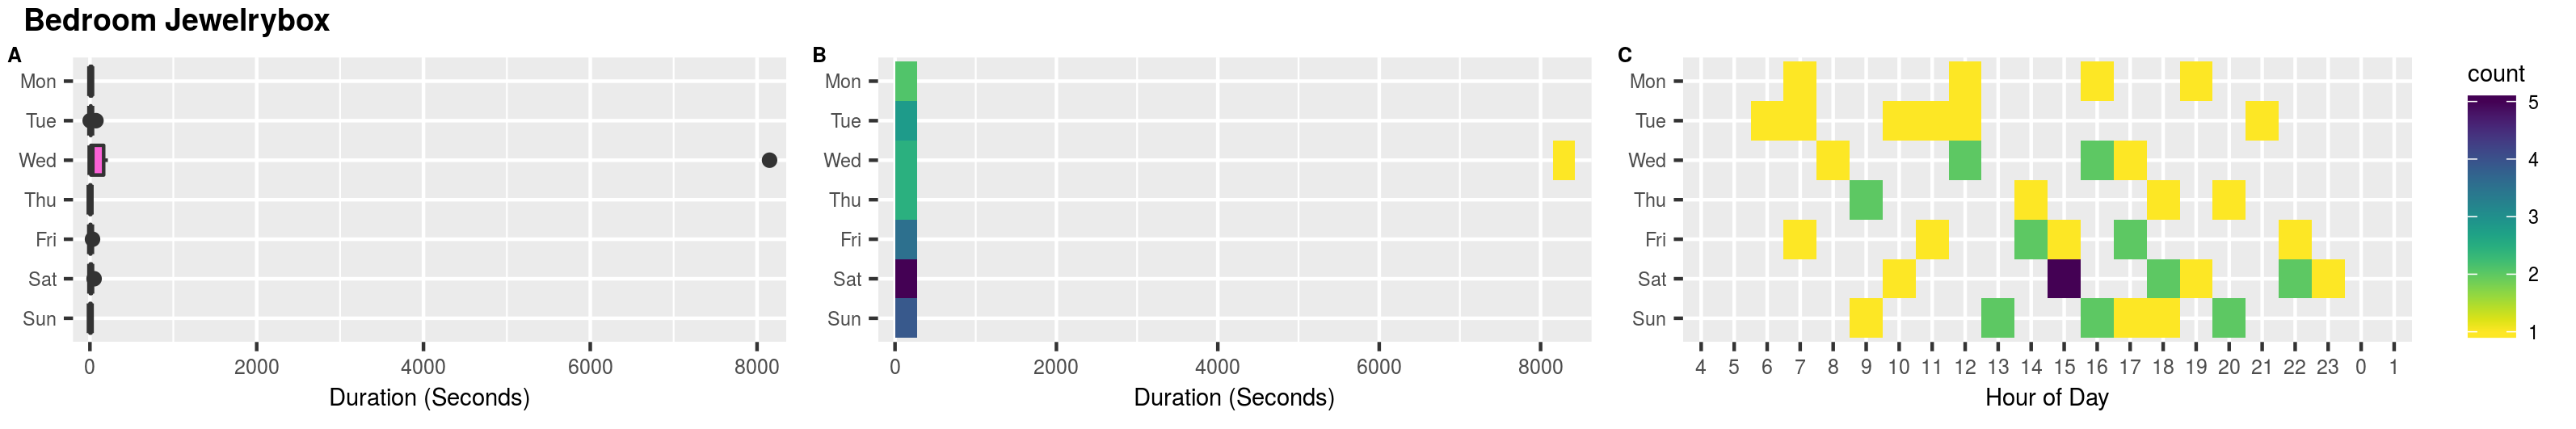
\includegraphics[width=1\linewidth]{/Users/alistairgj/Documents/GitHub/IoT_ResearchProject/IoT_November/images/subAct139} 

}

\caption{Box plot (A) and heat maps (B = day of week versus duration in seconds mapped by count, C = day of week versus hour of day mapped by count) for the Bedroom Jewelrybox sub activity.}\label{fig:subAct139}
\end{figure}

\hypertarget{the-final-pre-processed-dataset}{%
\subsubsection{The Final pre-processed
dataset}\label{the-final-pre-processed-dataset}}

XYZ

\hypertarget{data-analysis-and-manipulation}{%
\subsection{Data Analysis and
Manipulation}\label{data-analysis-and-manipulation}}

The primary focus of this section will be XYZ

\hypertarget{sequential-analysis-algorithm}{%
\subsubsection{Sequential Analysis
Algorithm}\label{sequential-analysis-algorithm}}

The following algorithm was created to evaluate the

\begin{Shaded}
\begin{Highlighting}[]
\KeywordTok{def}\NormalTok{ id_delta(events, n}\OperatorTok{=}\DecValTok{1}\NormalTok{, delta_threshold}\OperatorTok{=}\NormalTok{dt.timedelta(}\OperatorTok{-}\DecValTok{99}\NormalTok{)):}
\NormalTok{    nns }\OperatorTok{=}\NormalTok{ []}
    \ControlFlowTok{for}\NormalTok{ row }\KeywordTok{in}\NormalTok{ events.itertuples():}
\NormalTok{        start_time }\OperatorTok{=} \BuiltInTok{getattr}\NormalTok{(row, }\StringTok{'start'}\NormalTok{)}
\NormalTok{        end_time }\OperatorTok{=} \BuiltInTok{getattr}\NormalTok{(row, }\StringTok{'end'}\NormalTok{)}
\NormalTok{        subActNum }\OperatorTok{=} \BuiltInTok{getattr}\NormalTok{(row, }\StringTok{'subActNum'}\NormalTok{)}
\NormalTok{        row_index }\OperatorTok{=} \BuiltInTok{getattr}\NormalTok{(row, }\StringTok{'Index'}\NormalTok{)}
        
\NormalTok{        nn }\OperatorTok{=}\NormalTok{ events[(events.start }\OperatorTok{>=}\NormalTok{ start_time) }\OperatorTok{&} 
\NormalTok{                    (events.index }\OperatorTok{!=}\NormalTok{ row_index) }\OperatorTok{&} 
\NormalTok{                    ((start_time }\OperatorTok{-}\NormalTok{ events.start) }\OperatorTok{>}\NormalTok{ delta_threshold)][:n]}
        
\NormalTok{        ordered }\OperatorTok{=}\NormalTok{ pd.DataFrame()}
\NormalTok{        ordered[}\StringTok{'Dummy'}\NormalTok{] }\OperatorTok{=}\NormalTok{ nn[}\StringTok{'subActNum'}\NormalTok{]}
\NormalTok{        ordered[}\StringTok{'EventA'}\NormalTok{] }\OperatorTok{=}\NormalTok{ subActNum}
\NormalTok{        ordered[}\StringTok{'EventB'}\NormalTok{] }\OperatorTok{=}\NormalTok{ nn[}\StringTok{'subActNum'}\NormalTok{]}
\NormalTok{        ordered[}\StringTok{'EvA_Start'}\NormalTok{] }\OperatorTok{=}\NormalTok{ start_time}
\NormalTok{        ordered[}\StringTok{'EvB_Start'}\NormalTok{] }\OperatorTok{=}\NormalTok{ nn[}\StringTok{'start'}\NormalTok{]}
\NormalTok{        ordered[}\StringTok{'EvA_End'}\NormalTok{] }\OperatorTok{=}\NormalTok{ end_time}
\NormalTok{        ordered[}\StringTok{'EvB_End'}\NormalTok{] }\OperatorTok{=}\NormalTok{ nn[}\StringTok{'end'}\NormalTok{]}
        \KeywordTok{del}\NormalTok{ ordered[}\StringTok{'Dummy'}\NormalTok{]}
\NormalTok{        nns.append(ordered)}
  
    
\NormalTok{    result }\OperatorTok{=}\NormalTok{ pd.concat(nns)}
\NormalTok{    result[}\StringTok{'Delta'}\NormalTok{] }\OperatorTok{=}\NormalTok{ np.where(result[}\StringTok{'EvA_Start'}\NormalTok{]}\OperatorTok{==}\NormalTok{result[}\StringTok{'EvB_Start'}\NormalTok{], }
                               \DecValTok{0}\NormalTok{,}
\NormalTok{                               (result[}\StringTok{'EvB_Start'}\NormalTok{] }\OperatorTok{-}\NormalTok{ result[}\StringTok{'EvA_Start'}\NormalTok{]))}
\NormalTok{    result[}\StringTok{'Delta'}\NormalTok{] }\OperatorTok{=}\NormalTok{ result[}\StringTok{'Delta'}\NormalTok{].dt.total_seconds()}
    \ControlFlowTok{return}\NormalTok{ result}
\end{Highlighting}
\end{Shaded}

\pagebreak

\hypertarget{qualitative-sequential-analysis-via-sankey-diagram}{%
\subsubsection{Qualitative Sequential Analysis via Sankey
Diagram}\label{qualitative-sequential-analysis-via-sankey-diagram}}

\hypertarget{section}{%
\paragraph{}\label{section}}

\begin{figure}[H]

{\centering 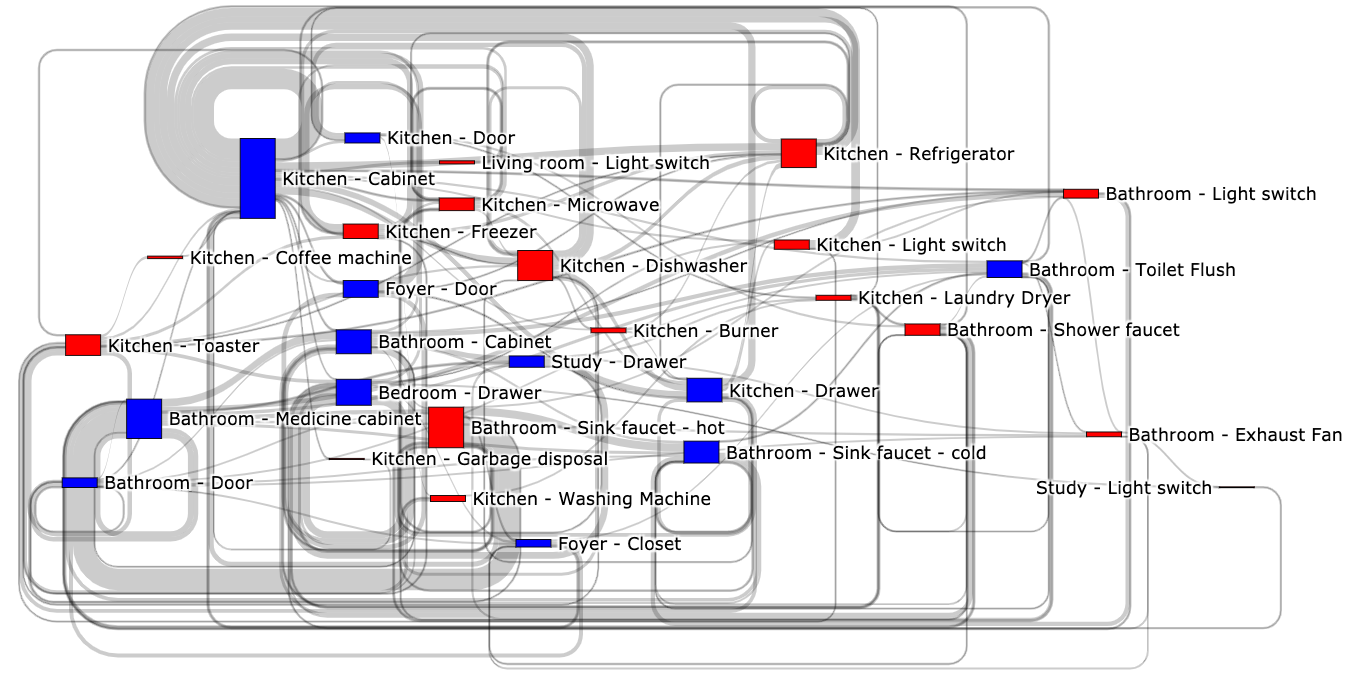
\includegraphics[width=1\linewidth]{/Users/alistairgj/Documents/GitHub/IoT_ResearchProject/IoT_November/images/WeekdayMorningds_1n_60s} 

}

\caption{Sankey Diagram of Weekday Mornings, considering all one neighbour per instance within a 60 second period}\label{fig:sankey_WeekdayMorningds_1n_60s}
\end{figure}

\begin{figure}[H]

{\centering 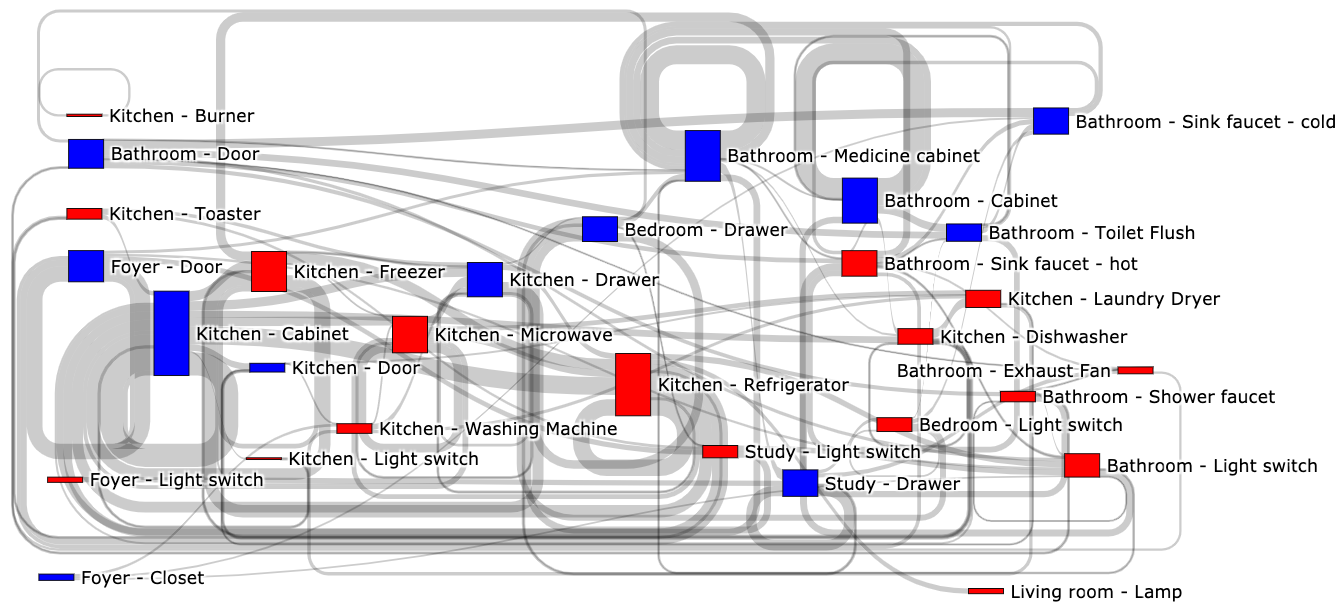
\includegraphics[width=1\linewidth]{/Users/alistairgj/Documents/GitHub/IoT_ResearchProject/IoT_November/images/WeekdayAfternoonds_1n_60s} 

}

\caption{Sankey Diagram of Weekday Afternoons, considering all one neighbour per instance within a 60 second period}\label{fig:sankey_WeekdayAfternoonds_1n_60s}
\end{figure}

\begin{figure}[H]

{\centering 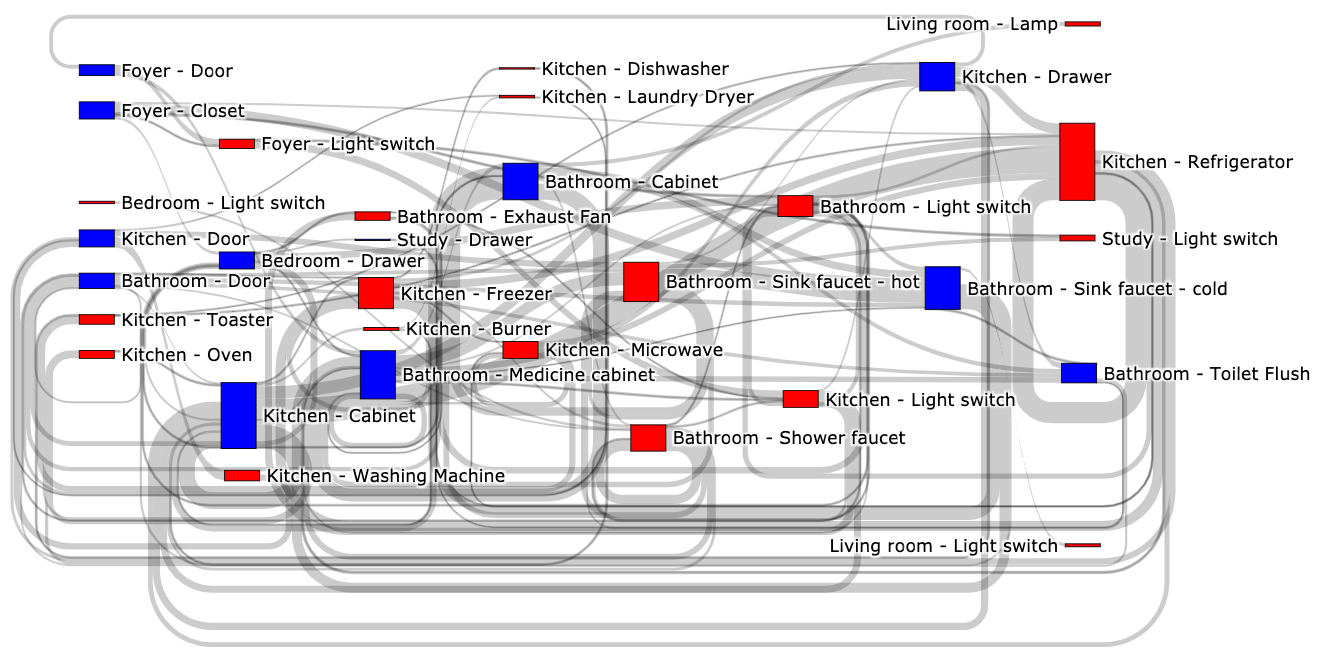
\includegraphics[width=1\linewidth]{/Users/alistairgj/Documents/GitHub/IoT_ResearchProject/IoT_November/images/WeekdayEveningds_1n_60s} 

}

\caption{Sankey Diagram of Weekday Evenings, considering all one neighbour per instance within a 60 second period}\label{fig:sankey_WeekdayEveningds_1n_60s}
\end{figure}

\begin{figure}[H]

{\centering 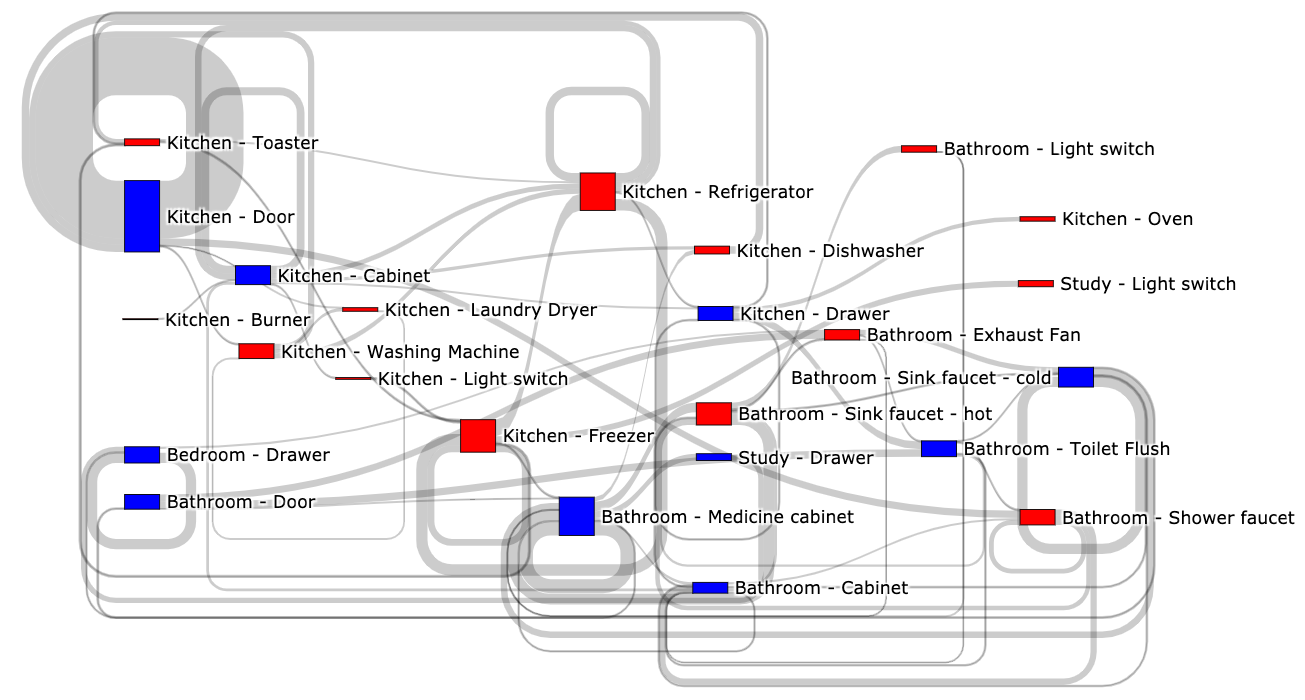
\includegraphics[width=1\linewidth]{/Users/alistairgj/Documents/GitHub/IoT_ResearchProject/IoT_November/images/WeekendMorningds_1n_60s} 

}

\caption{Sankey Diagram of Weekend Mornings, considering all one neighbour per instance within a 60 second period}\label{fig:sankey_WeekendMorningds_1n_60s}
\end{figure}

\begin{figure}[H]

{\centering 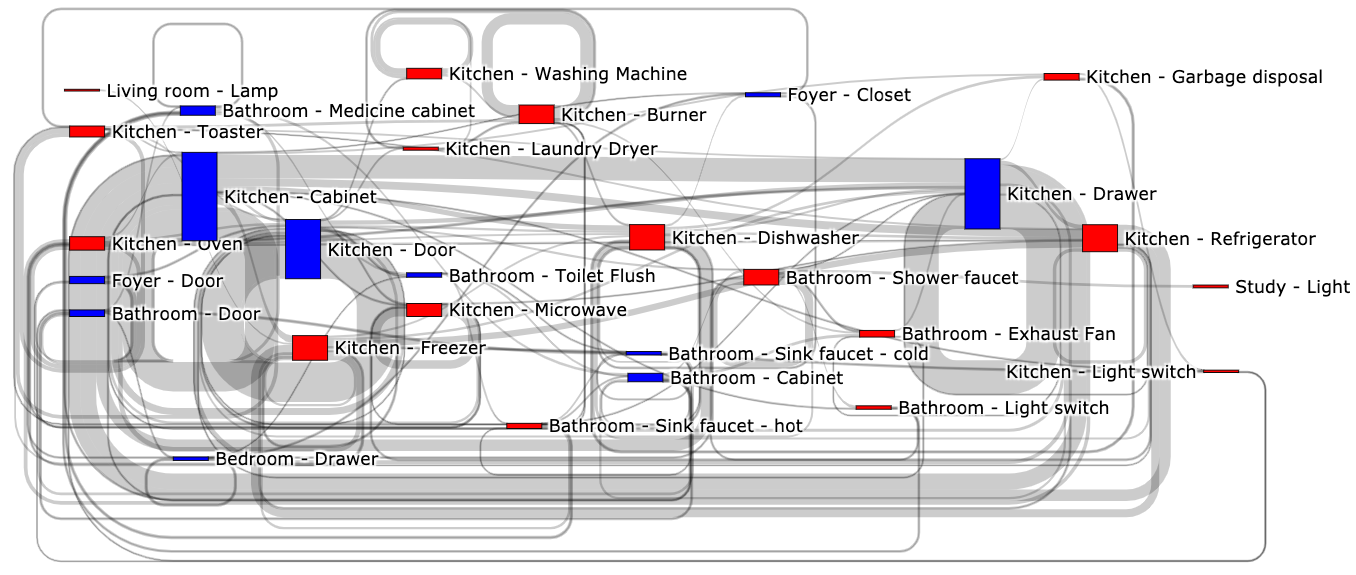
\includegraphics[width=1\linewidth]{/Users/alistairgj/Documents/GitHub/IoT_ResearchProject/IoT_November/images/WeekendAfternoonds_1n_60s} 

}

\caption{Sankey Diagram of Weekend Afternoons, considering all one neighbour per instance within a 60 second period}\label{fig:sankey_WeekendAfternoonds_1n_60s}
\end{figure}

\begin{figure}[H]

{\centering 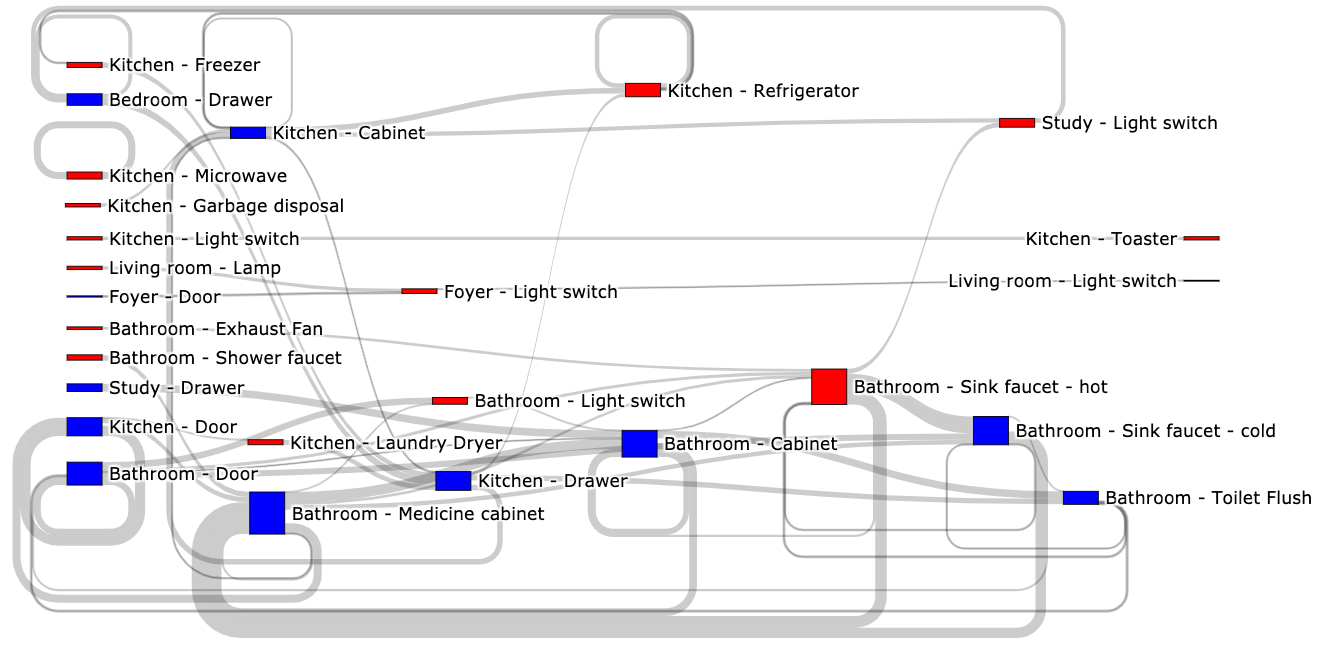
\includegraphics[width=1\linewidth]{/Users/alistairgj/Documents/GitHub/IoT_ResearchProject/IoT_November/images/WeekendEveningds_1n_60s} 

}

\caption{Sankey Diagram of Weekend Evenings, considering all one neighbour per instance within a 60 second period}\label{fig:sankey_WeekendEveningds_1n_60s}
\end{figure}

\pagebreak

Test for in \ref{fig:fig1} we see XYZ

\begin{figure}[H]

{\centering 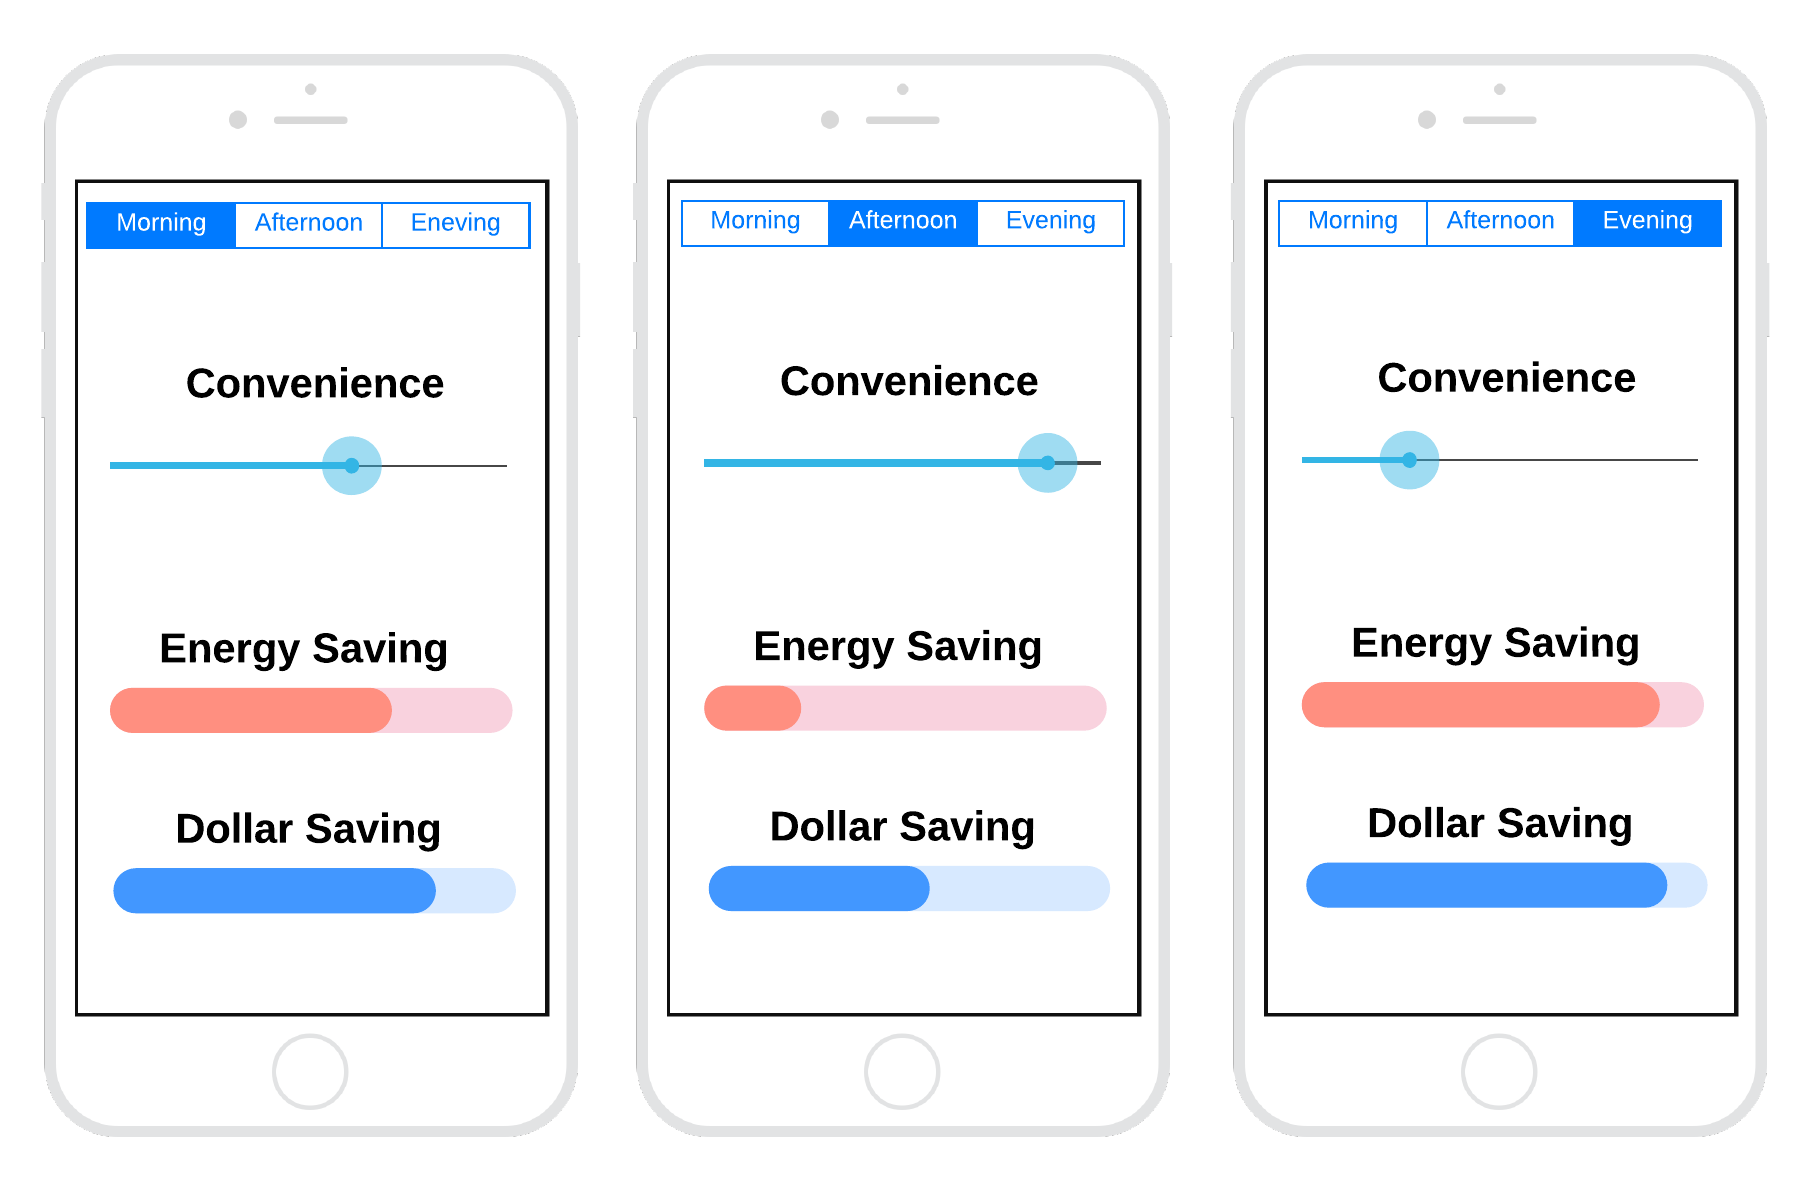
\includegraphics[width=0.8\linewidth]{/Users/alistairgj/Documents/GitHub/IoT_ResearchProject/IoT_November/images/iosMockUps} 

}

\caption{ADD TEXT}\label{fig:unnamed-chunk-12}
\end{figure}

\pagebreak

\pagebreak

\hypertarget{bedroom-lamp---subact64}{%
\paragraph{Bedroom Lamp - SubAct64}\label{bedroom-lamp---subact64}}

The bedroom lamp was only present in the dataset for one instance, as
seen in Figure \ref{fig:subAct64}, and thus this sub activity was
dropped from the dataset.

\hypertarget{kitchen-cereal---subact145}{%
\paragraph{Kitchen Cereal -
SubAct145}\label{kitchen-cereal---subact145}}

Likewise with the bedroom jewelry box, the kitchen cereal subactivity,
Figure \ref{fig:subAct145} below, was dropped due to the extremely
specific nature of this activity.

\hypertarget{kitchen-containers---subact60}{%
\paragraph{Kitchen Containers -
SubAct60}\label{kitchen-containers---subact60}}

Likewise with the bedroom jewelry box, the kitchen containers
subactivity, Figure \ref{fig:subAct60} below, was dropped due to the
extremely specific nature of this activity.

\hypertarget{foyer-closet---subact81}{%
\paragraph{Foyer Closet - subAct81}\label{foyer-closet---subact81}}

\begin{figure}[H]

{\centering 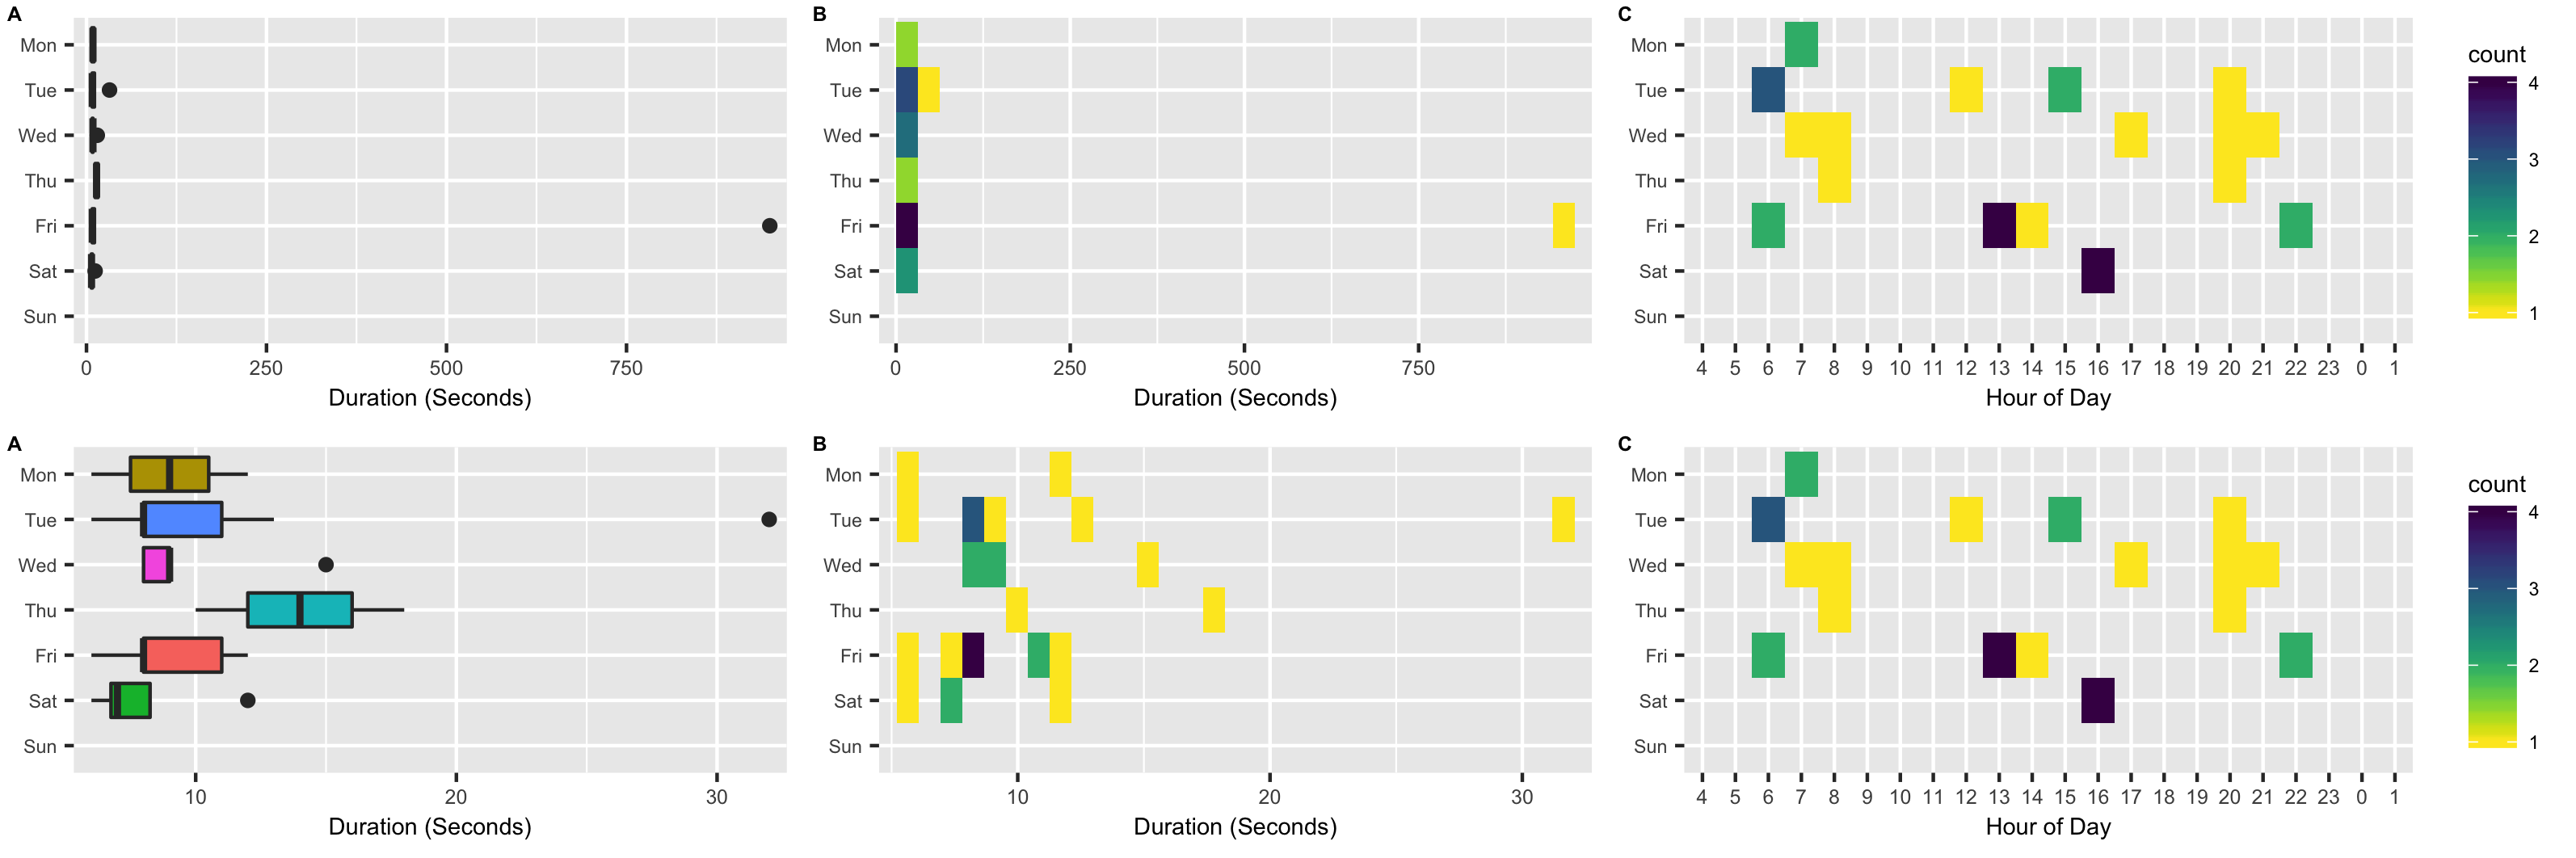
\includegraphics[width=1\linewidth]{/Users/alistairgj/Documents/GitHub/IoT_ResearchProject/IoT_November/images/subAct81} 

}

\caption{Box plot (A) and heat maps (B = day of week versus duration in seconds mapped by count, C = day of week versus hour of day mapped by count) for the Foyer Closet sub activity.}\label{fig:subAct81}
\end{figure}

\hypertarget{bathroom-medicine-cabinet}{%
\paragraph{Bathroom Medicine Cabinet}\label{bathroom-medicine-cabinet}}

\begin{figure}[H]

{\centering 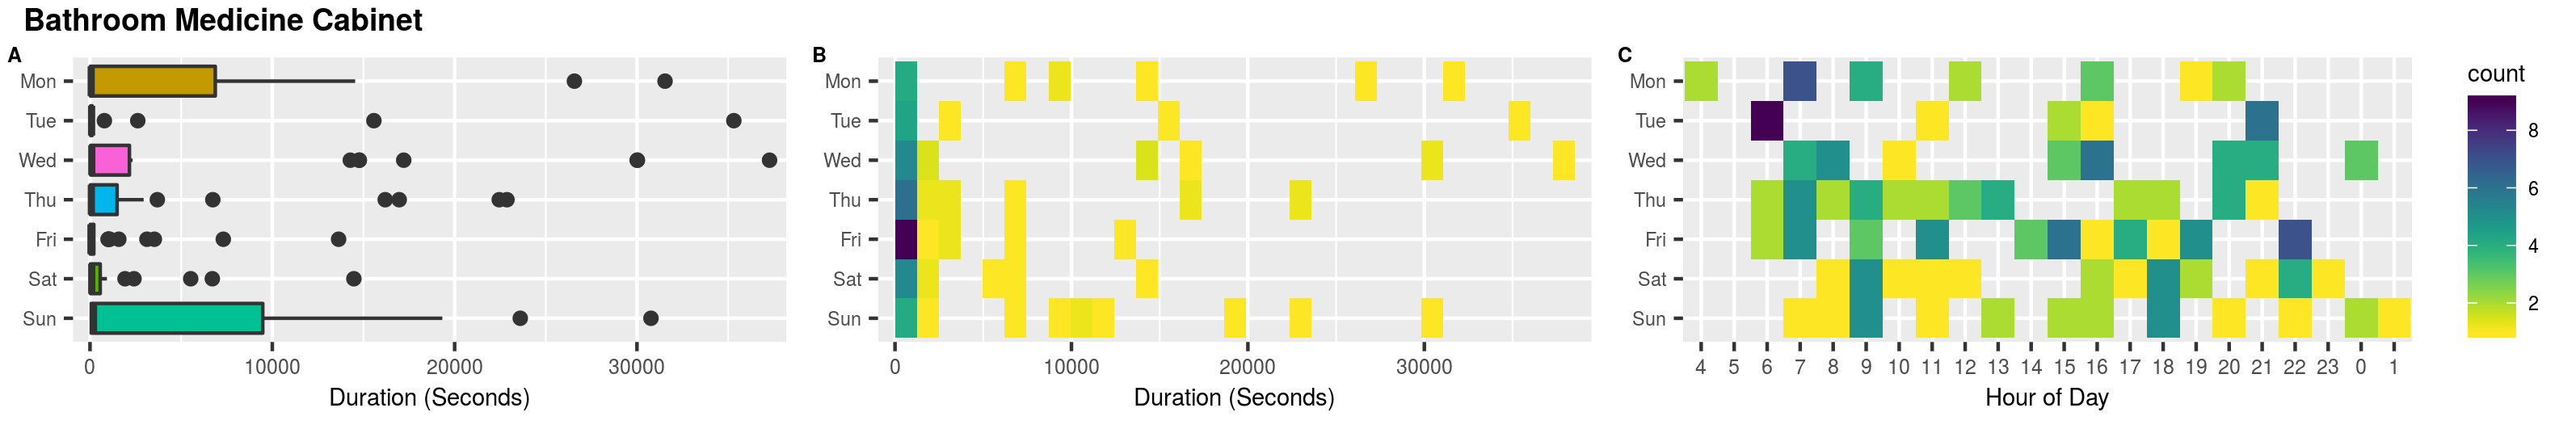
\includegraphics[width=1\linewidth]{/Users/alistairgj/Documents/GitHub/IoT_ResearchProject/IoT_November/images/subAct57} 

}

\caption{A caption}\label{fig:subAct57}
\end{figure}

\hypertarget{study-drawer}{%
\paragraph{Study Drawer}\label{study-drawer}}

\begin{figure}[H]

{\centering 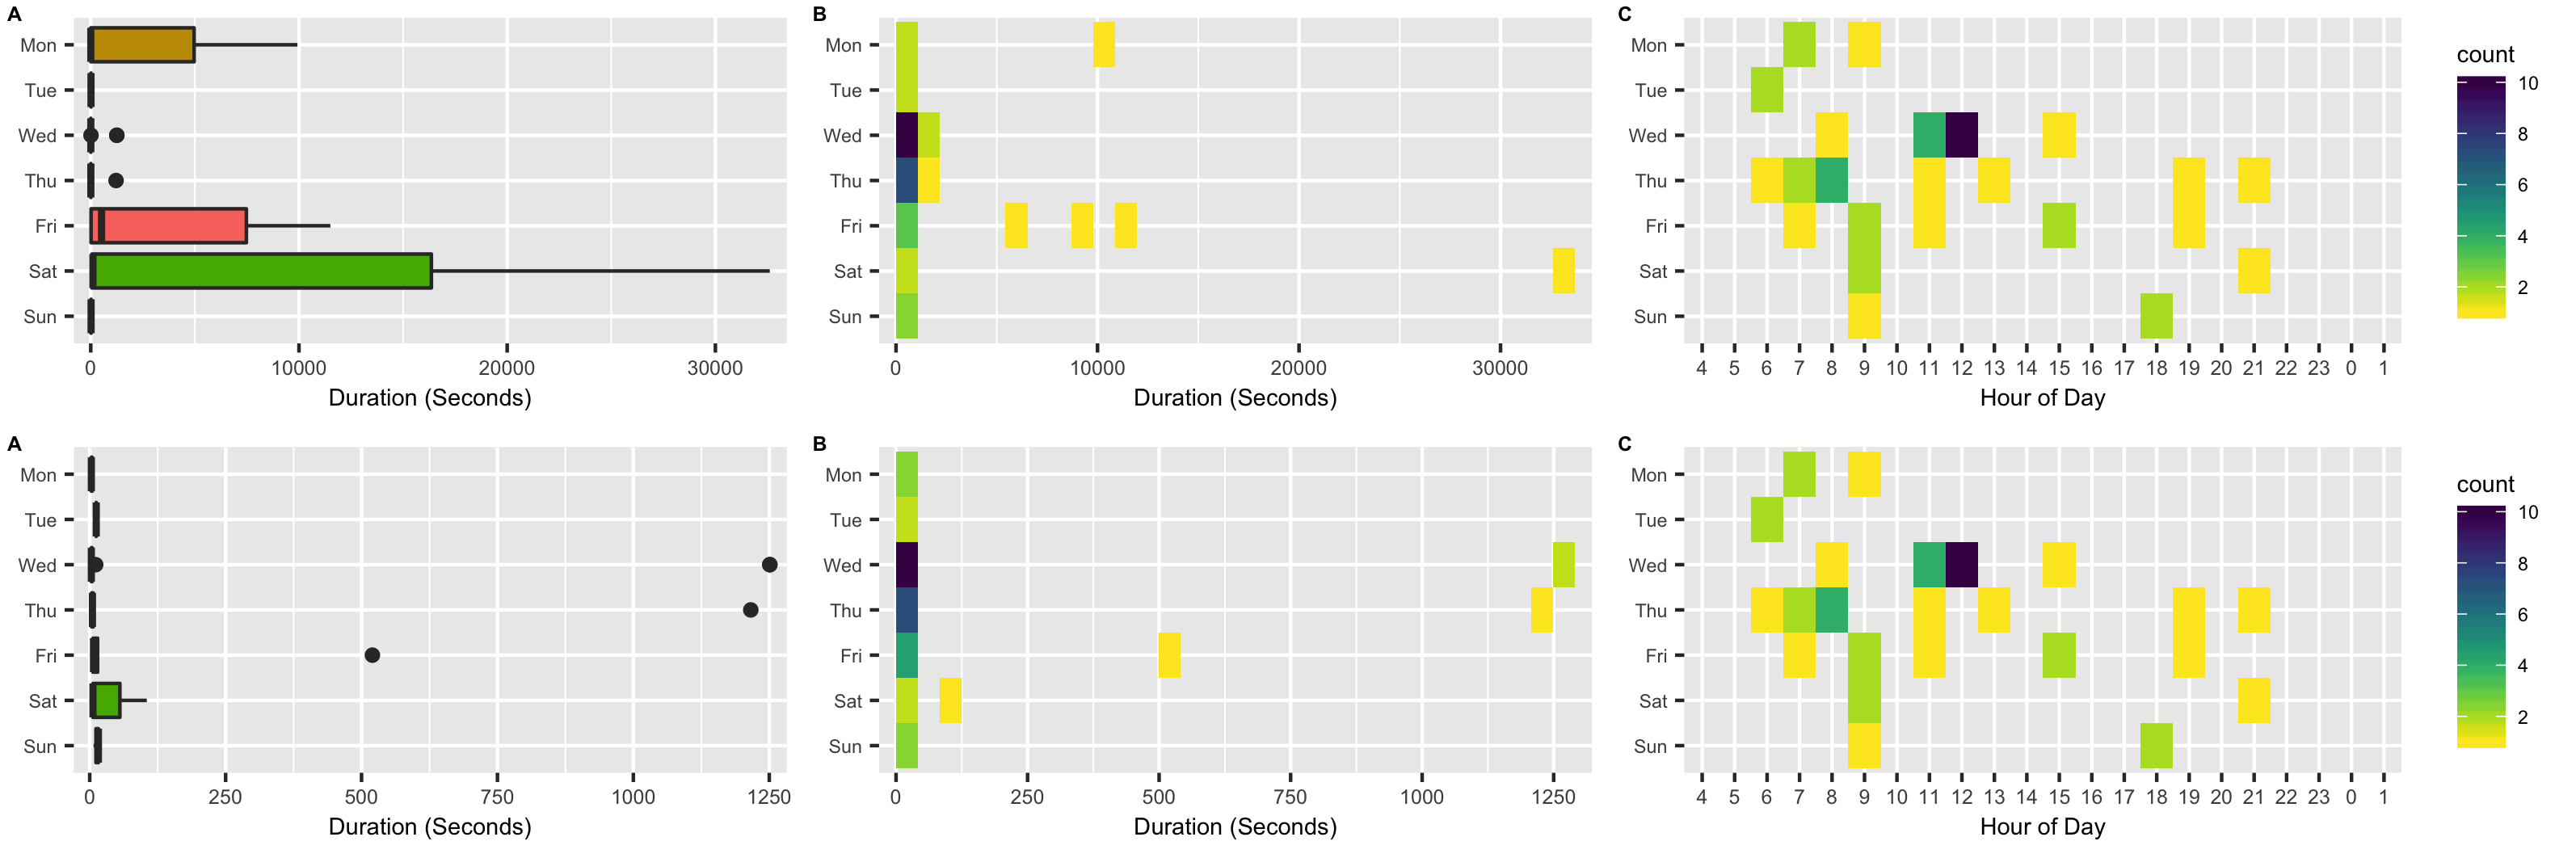
\includegraphics[width=1\linewidth]{/Users/alistairgj/Documents/GitHub/IoT_ResearchProject/IoT_November/images/subAct82} 

}

\caption{A caption}\label{fig:subAct82}
\end{figure}

\hypertarget{bedroom-drawer}{%
\paragraph{Bedroom Drawer}\label{bedroom-drawer}}

\begin{figure}[H]

{\centering 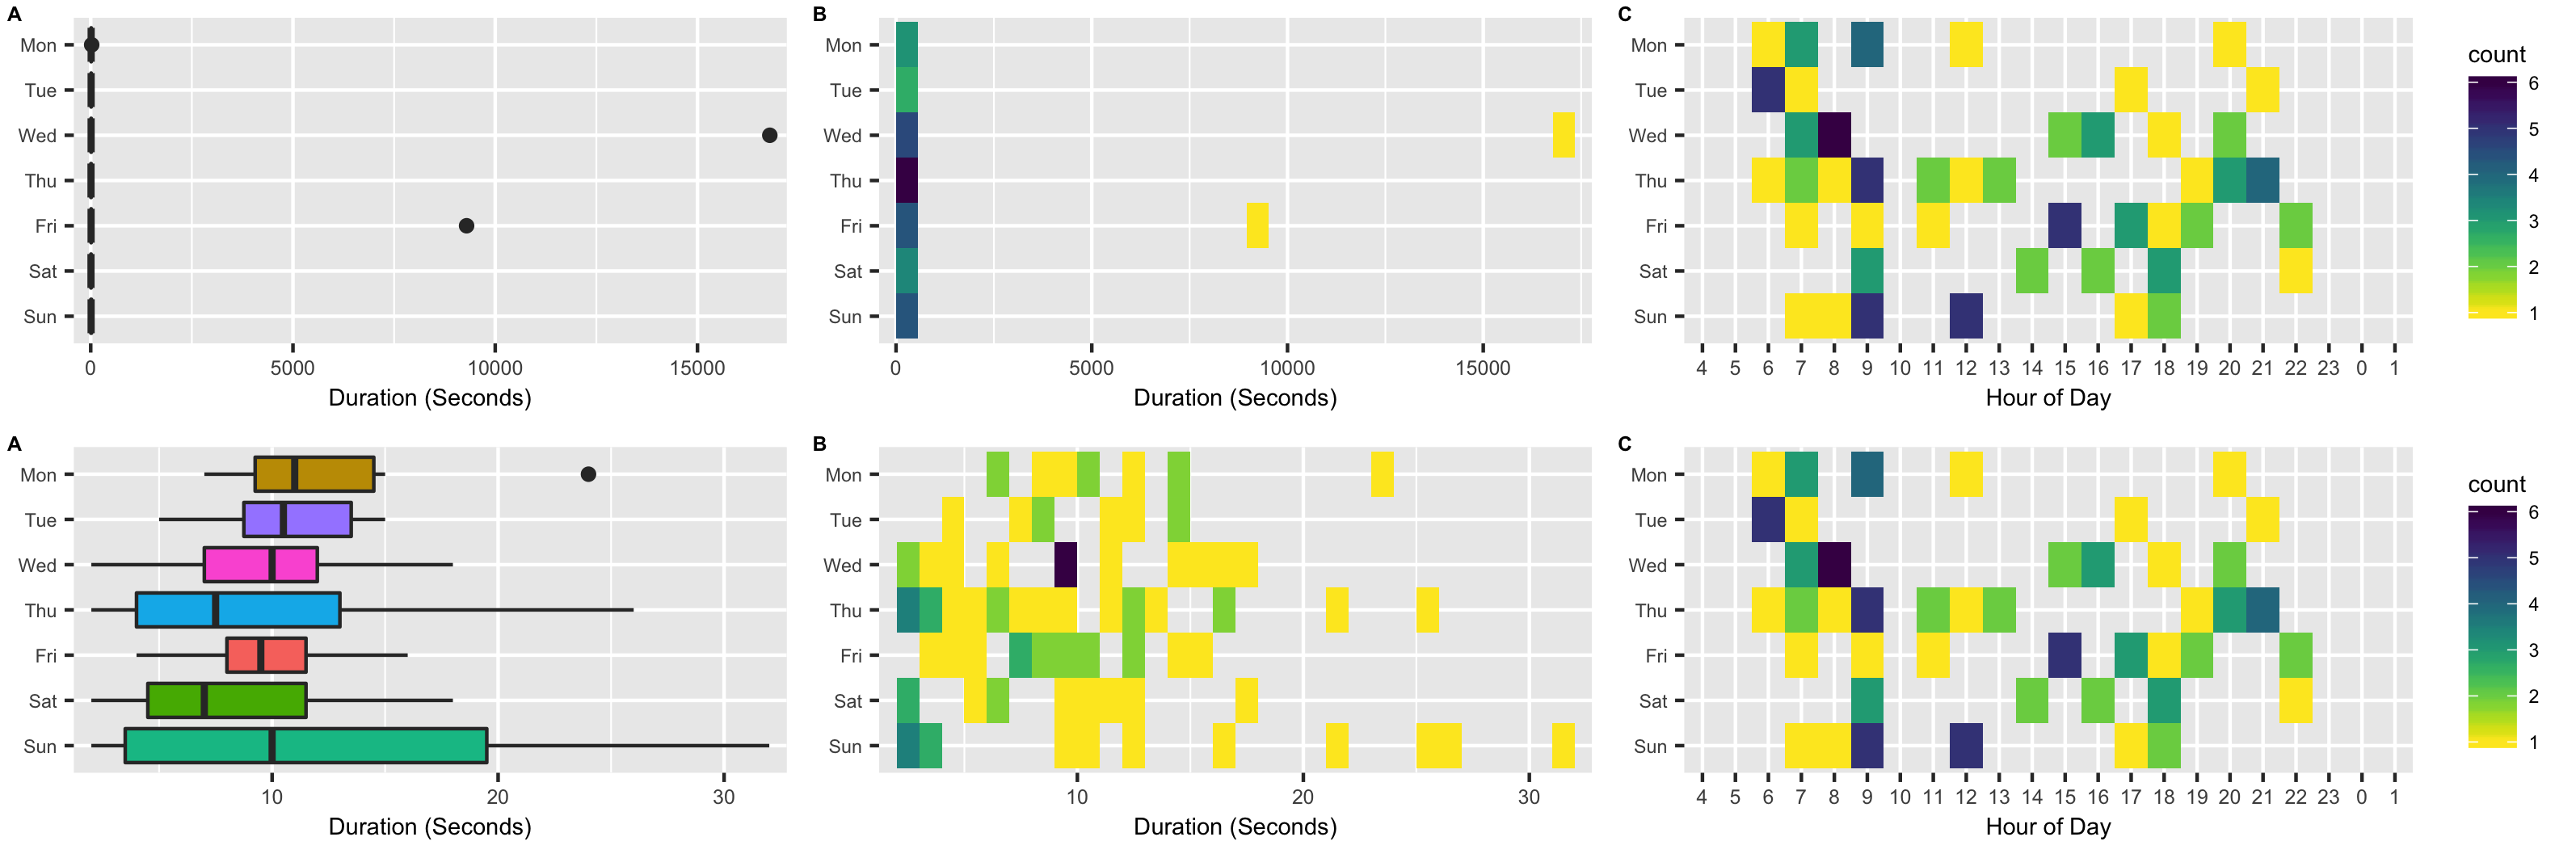
\includegraphics[width=1\linewidth]{/Users/alistairgj/Documents/GitHub/IoT_ResearchProject/IoT_November/images/subAct146} 

}

\caption{A caption}\label{fig:subAct146}
\end{figure}

\hypertarget{kitchen-cabinet}{%
\paragraph{Kitchen Cabinet}\label{kitchen-cabinet}}

\begin{figure}[H]

{\centering 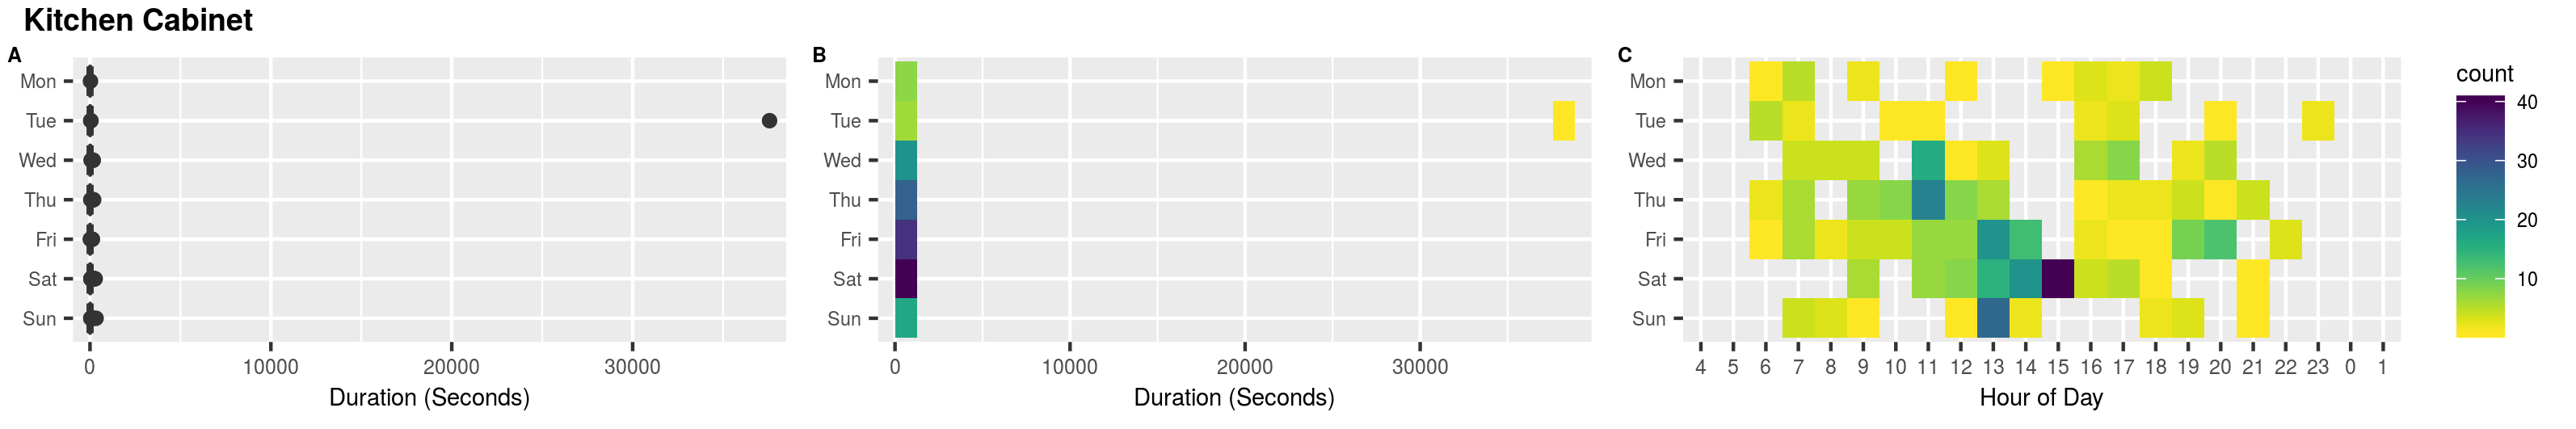
\includegraphics[width=1\linewidth]{/Users/alistairgj/Documents/GitHub/IoT_ResearchProject/IoT_November/images/subAct132} 

}

\caption{A caption}\label{fig:subAct132}
\end{figure}

\hypertarget{kitchen-microwave}{%
\paragraph{Kitchen Microwave}\label{kitchen-microwave}}

\begin{figure}[H]

{\centering 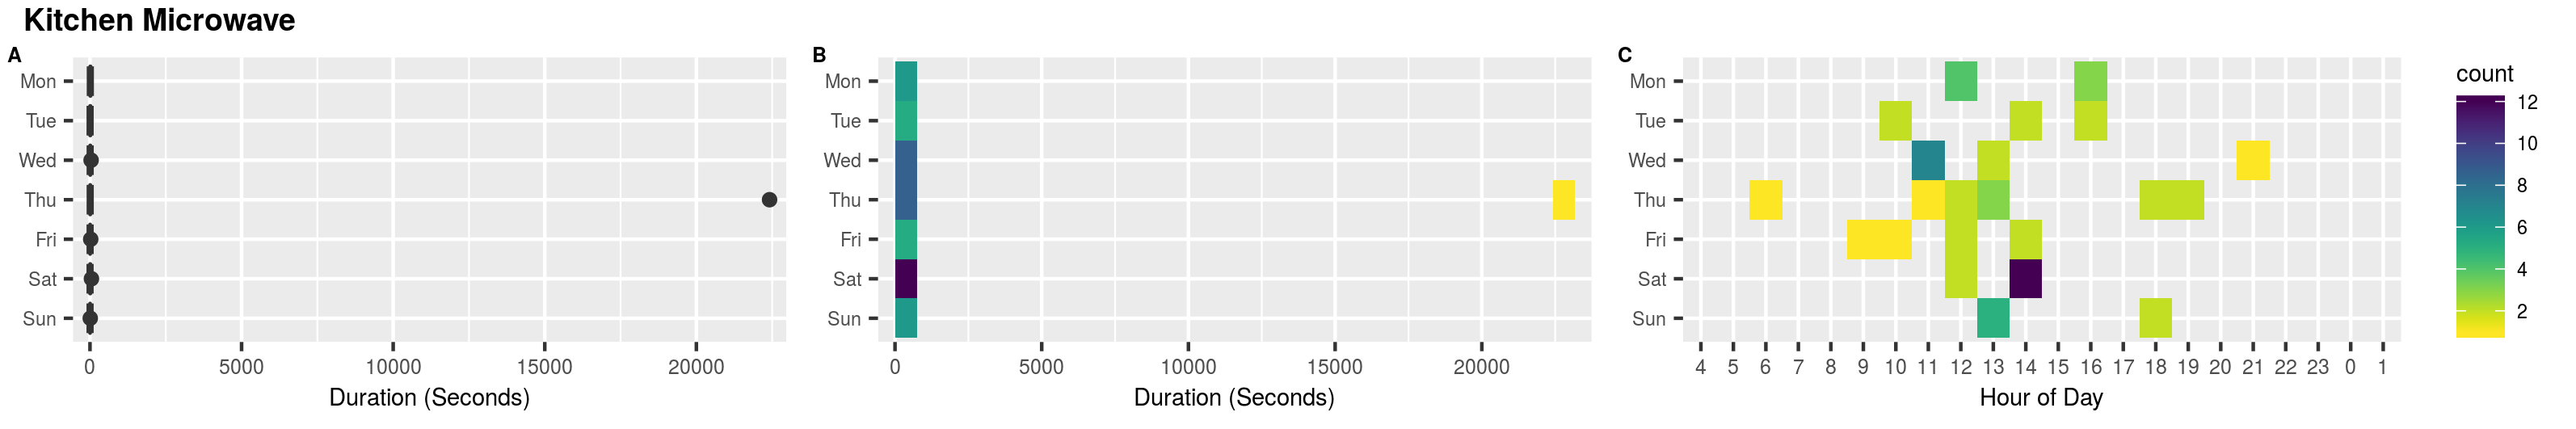
\includegraphics[width=1\linewidth]{/Users/alistairgj/Documents/GitHub/IoT_ResearchProject/IoT_November/images/subAct143} 

}

\caption{A caption}\label{fig:subAct143}
\end{figure}

\hypertarget{kitchen-door}{%
\paragraph{Kitchen Door}\label{kitchen-door}}

\begin{figure}[H]

{\centering 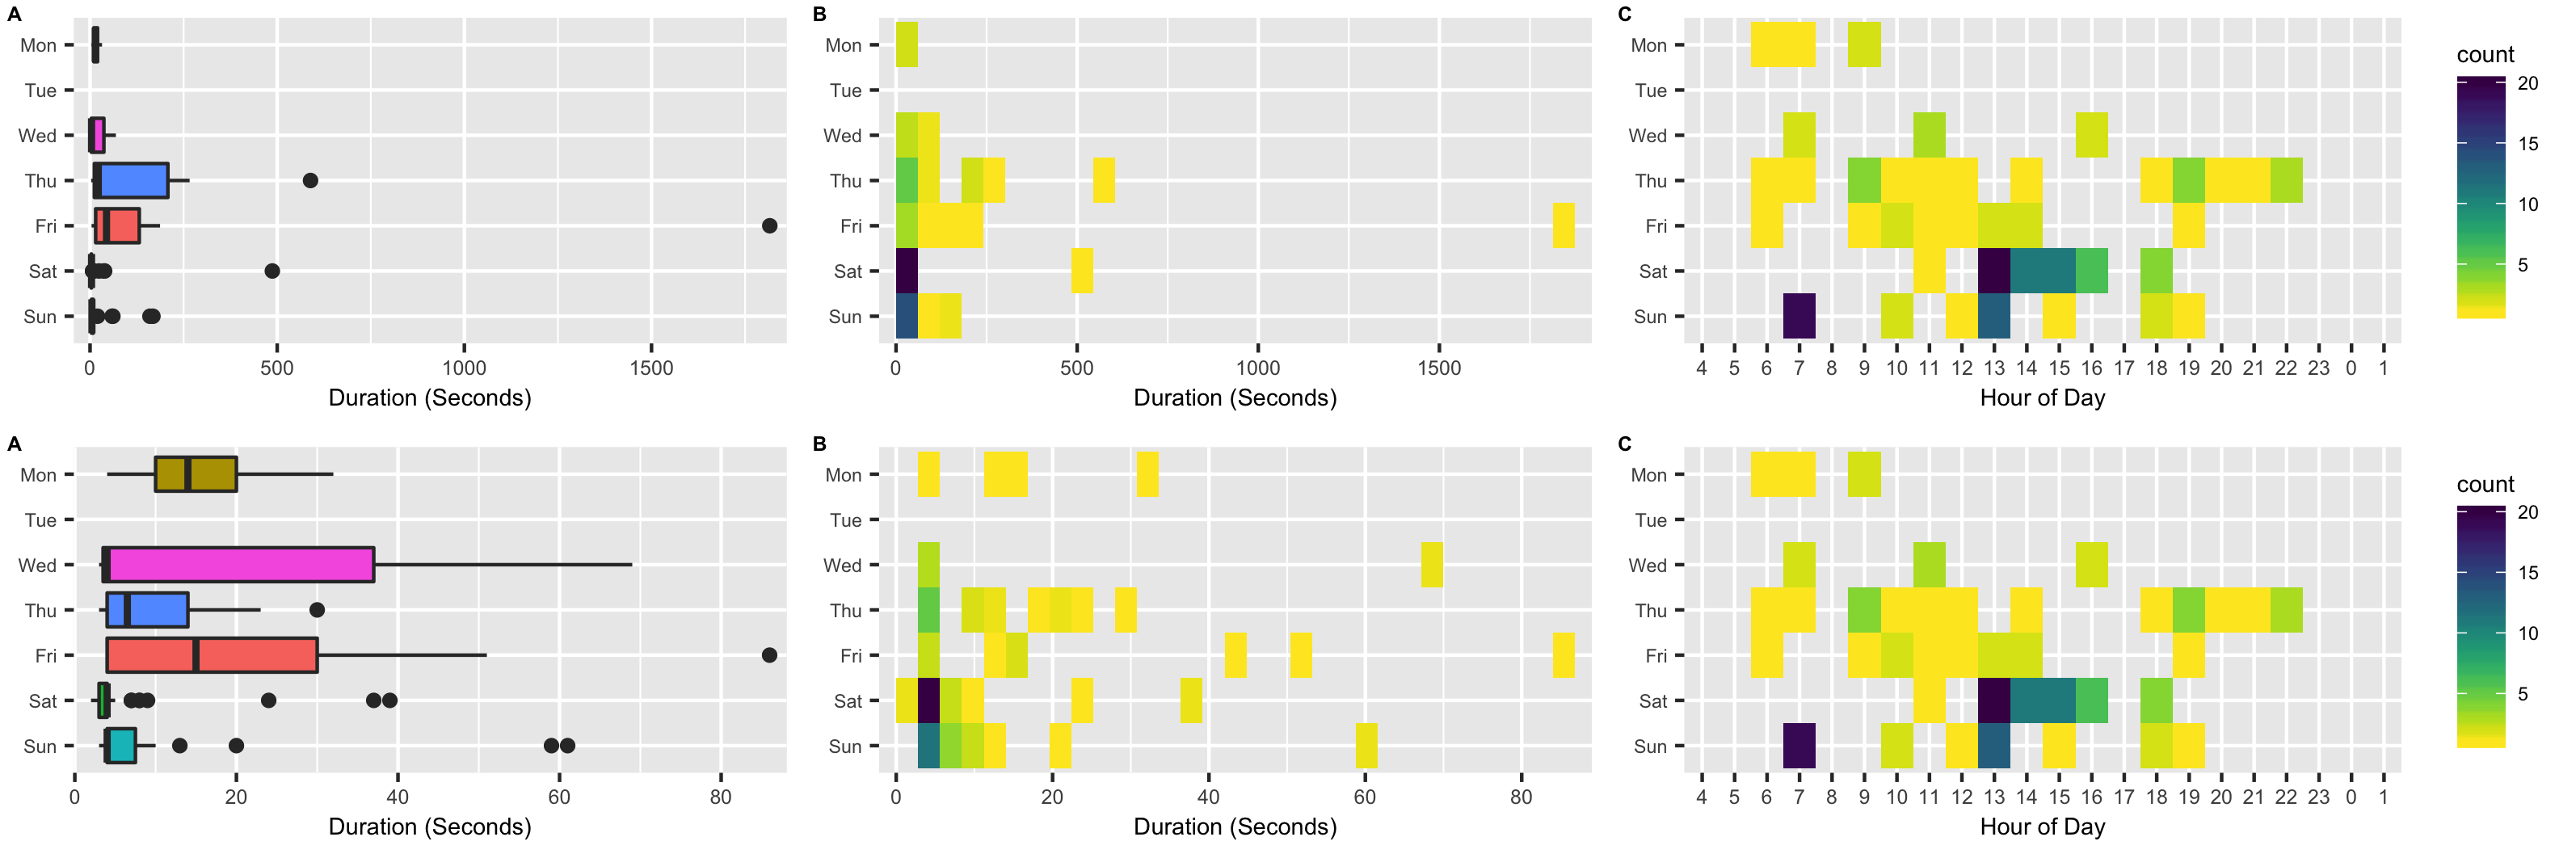
\includegraphics[width=1\linewidth]{/Users/alistairgj/Documents/GitHub/IoT_ResearchProject/IoT_November/images/subAct141} 

}

\caption{A caption}\label{fig:subAct141}
\end{figure}

\hypertarget{bathroom-shower-faucet}{%
\paragraph{Bathroom Shower Faucet}\label{bathroom-shower-faucet}}

\begin{figure}[H]

{\centering 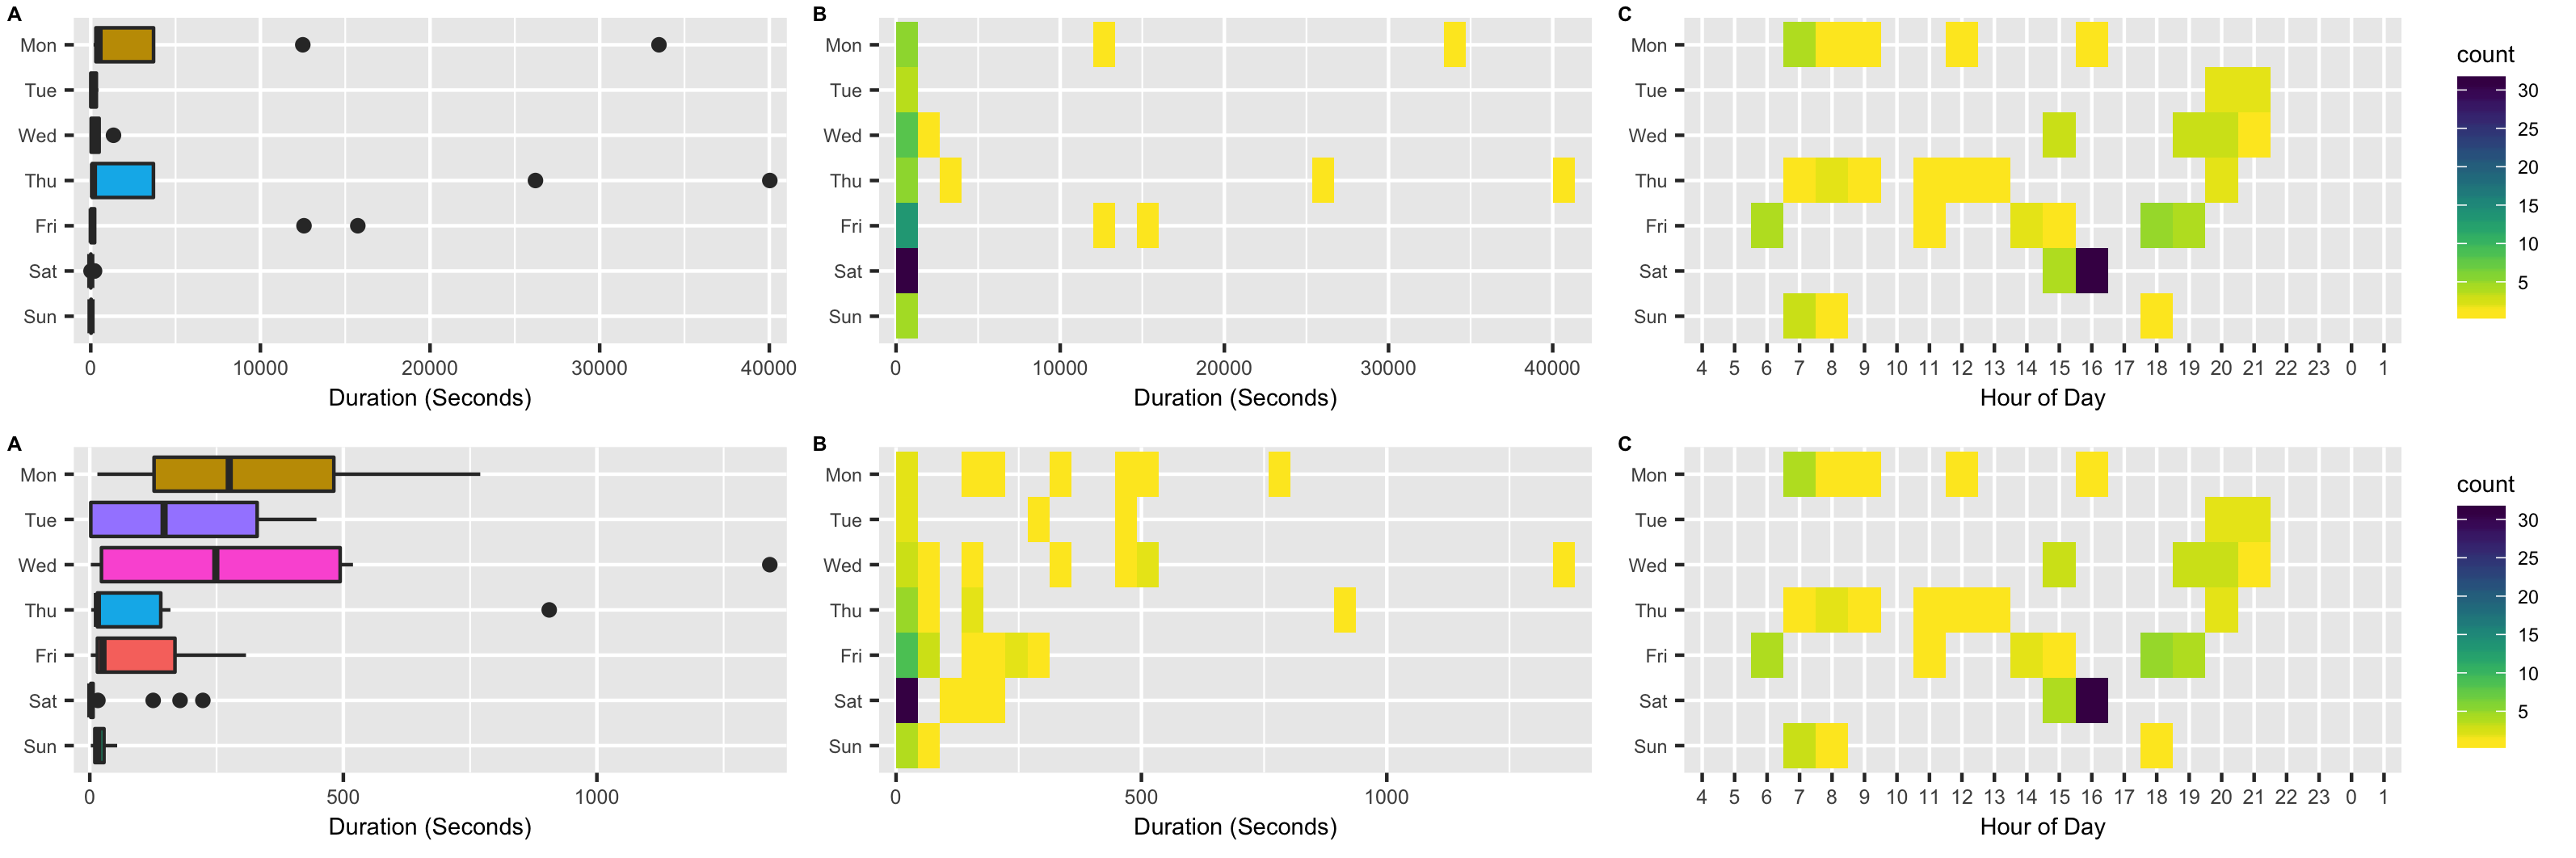
\includegraphics[width=1\linewidth]{/Users/alistairgj/Documents/GitHub/IoT_ResearchProject/IoT_November/images/subAct93} 

}

\caption{A caption}\label{fig:subAct93}
\end{figure}

\hypertarget{kitchen-drawer}{%
\paragraph{Kitchen Drawer}\label{kitchen-drawer}}

\begin{figure}[H]

{\centering 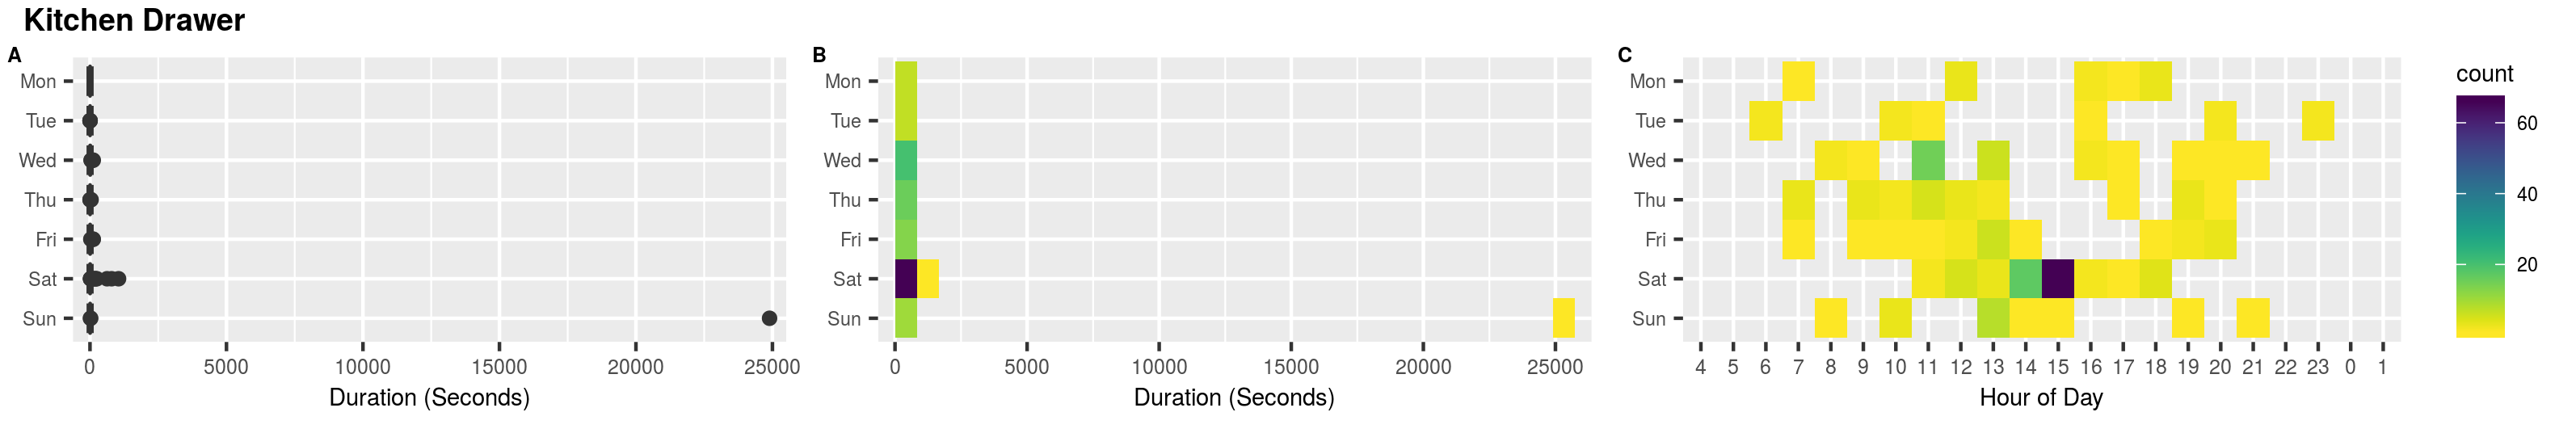
\includegraphics[width=1\linewidth]{/Users/alistairgj/Documents/GitHub/IoT_ResearchProject/IoT_November/images/subAct125} 

}

\caption{A caption}\label{fig:subAct125}
\end{figure}

\hypertarget{kitchen-dishwasher}{%
\paragraph{Kitchen Dishwasher}\label{kitchen-dishwasher}}

\begin{figure}[H]

{\centering 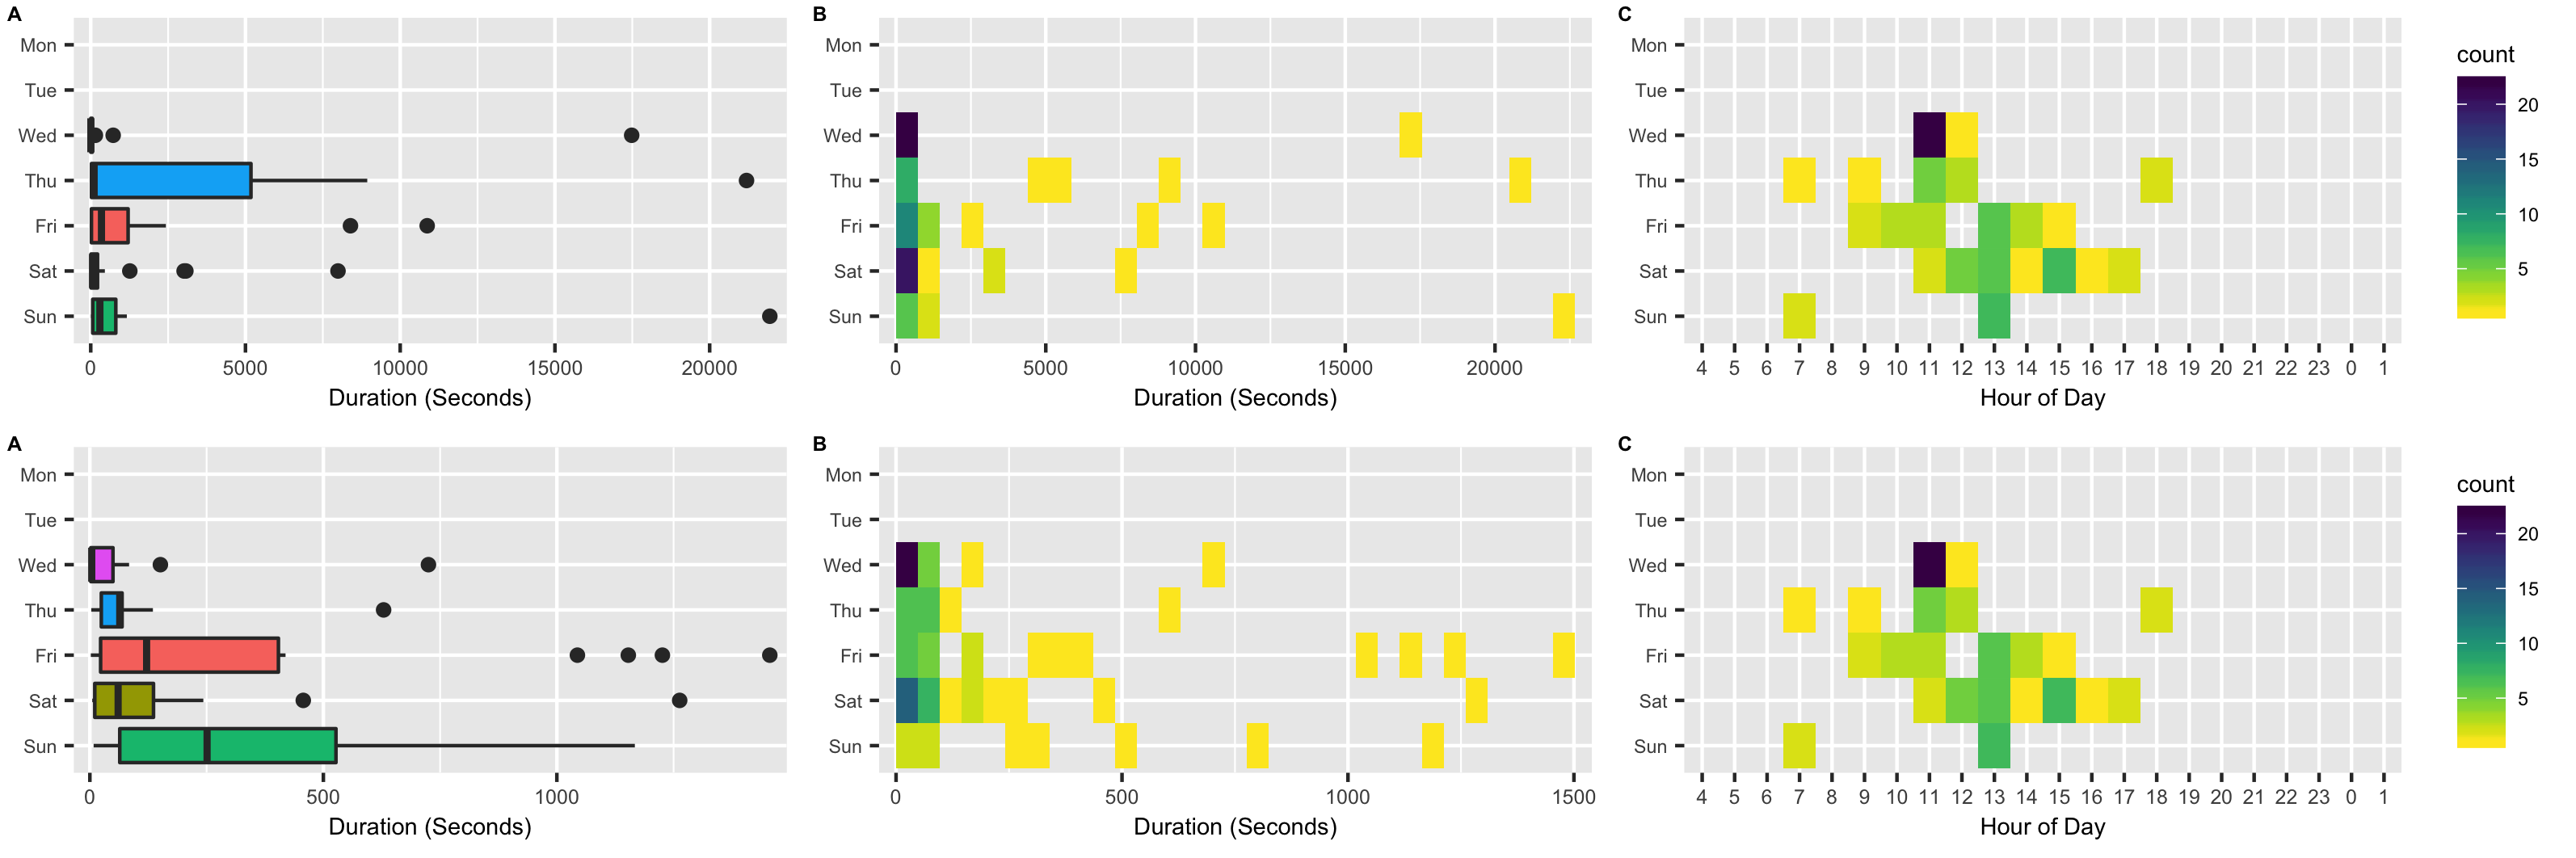
\includegraphics[width=1\linewidth]{/Users/alistairgj/Documents/GitHub/IoT_ResearchProject/IoT_November/images/subAct70} 

}

\caption{A caption}\label{fig:subAct70}
\end{figure}

\hypertarget{kitchen-refrigerator}{%
\paragraph{Kitchen Refrigerator}\label{kitchen-refrigerator}}

\begin{figure}[H]

{\centering 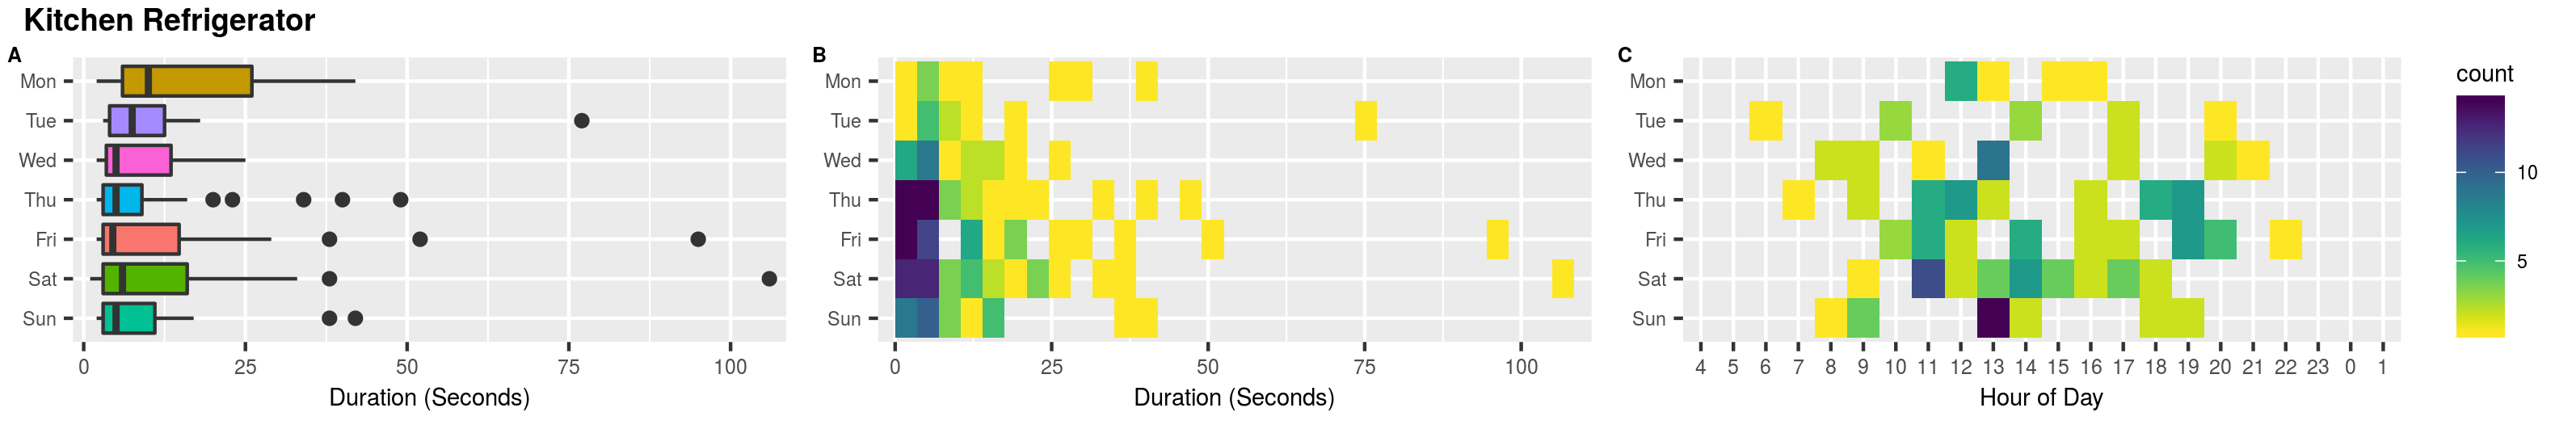
\includegraphics[width=1\linewidth]{/Users/alistairgj/Documents/GitHub/IoT_ResearchProject/IoT_November/images/subAct126} 

}

\caption{A caption}\label{fig:subAct126}
\end{figure}

\hypertarget{bathroom-sink-faucet---cold}{%
\paragraph{Bathroom Sink Faucet -
Cold}\label{bathroom-sink-faucet---cold}}

\begin{figure}[H]

{\centering 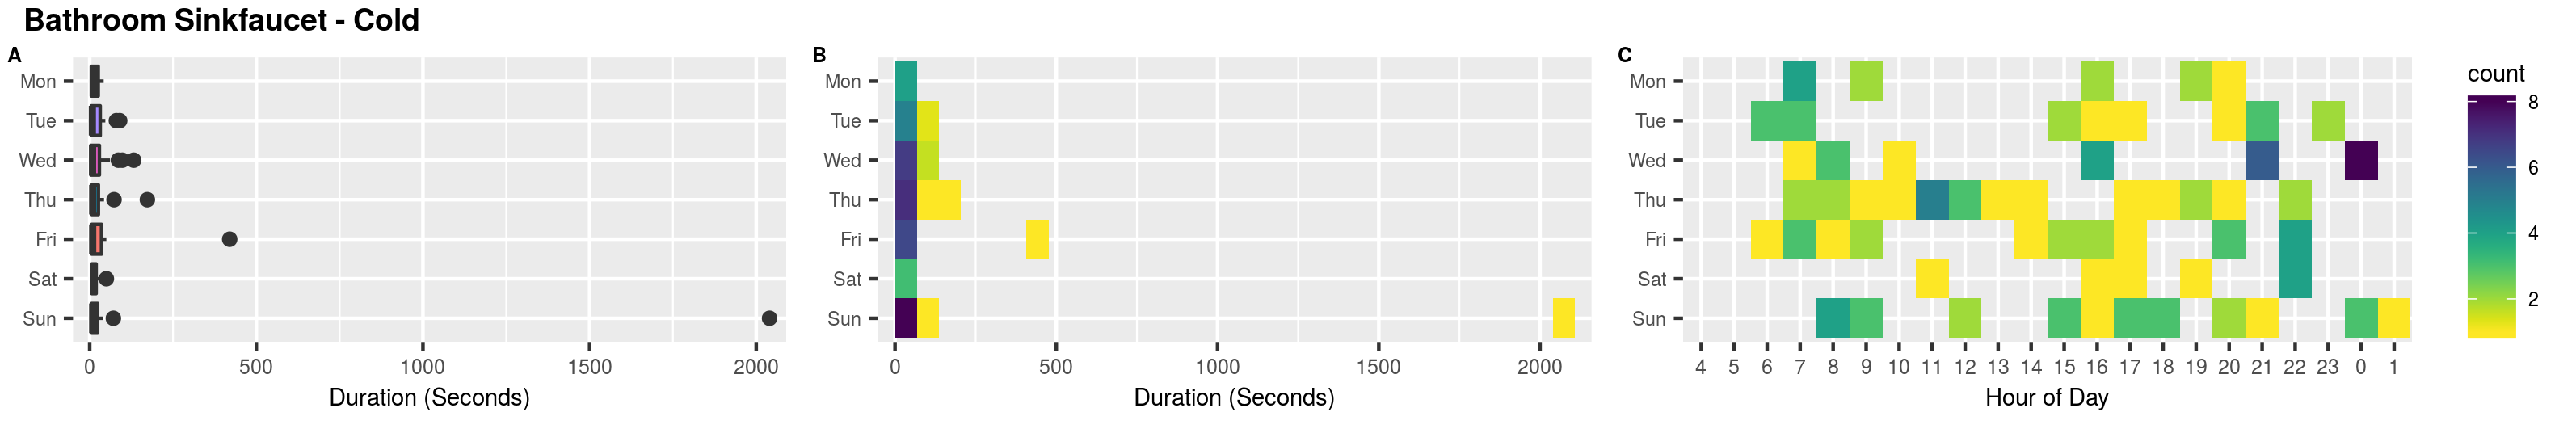
\includegraphics[width=1\linewidth]{/Users/alistairgj/Documents/GitHub/IoT_ResearchProject/IoT_November/images/subAct88} 

}

\caption{A caption}\label{fig:subAct88}
\end{figure}

\hypertarget{bathroom-sink-faucet---hot}{%
\paragraph{Bathroom Sink Faucet -
Hot}\label{bathroom-sink-faucet---hot}}

\begin{figure}[H]

{\centering 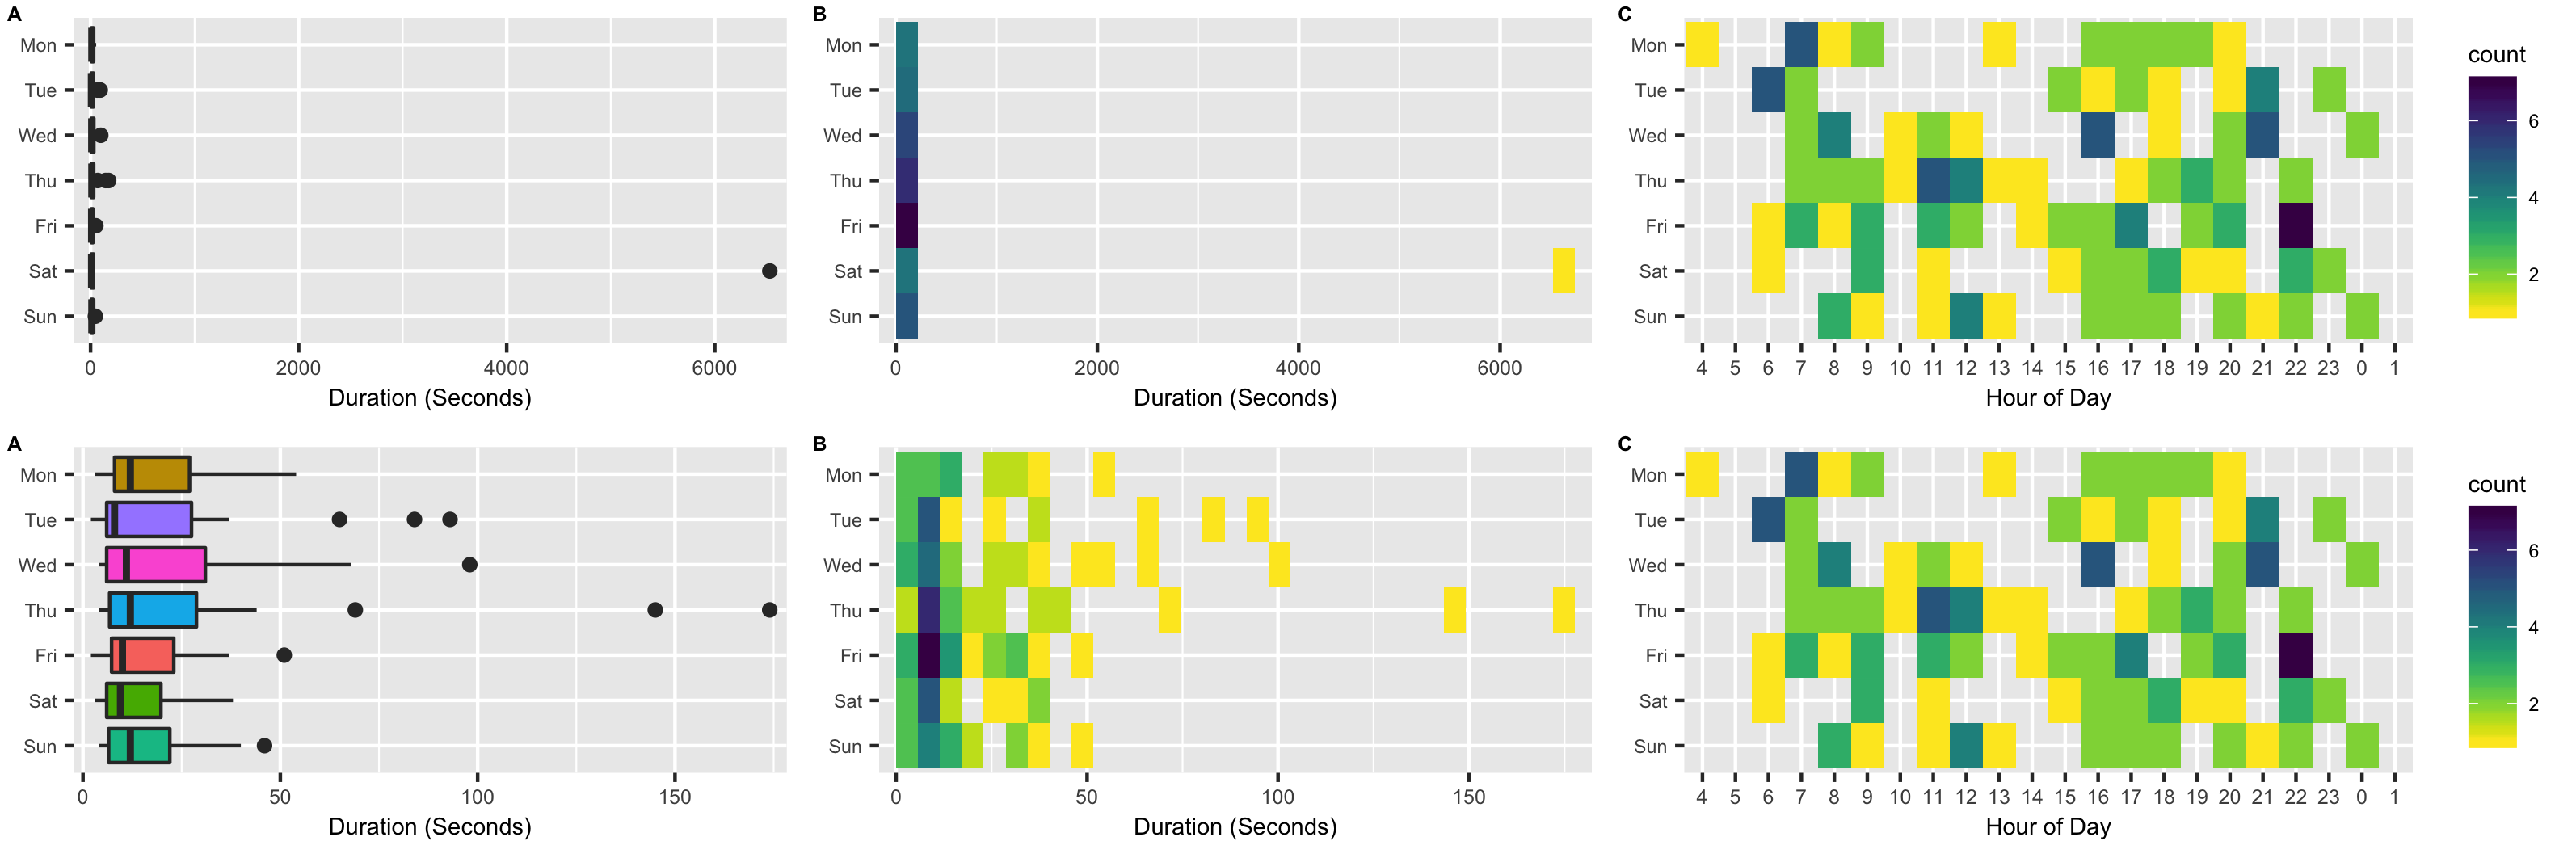
\includegraphics[width=1\linewidth]{/Users/alistairgj/Documents/GitHub/IoT_ResearchProject/IoT_November/images/subAct68} 

}

\caption{A caption}\label{fig:subAct68}
\end{figure}

\hypertarget{foyer-door-subactnum-140}{%
\paragraph{Foyer Door (SubActNum 140)}\label{foyer-door-subactnum-140}}

\begin{figure}[H]

{\centering 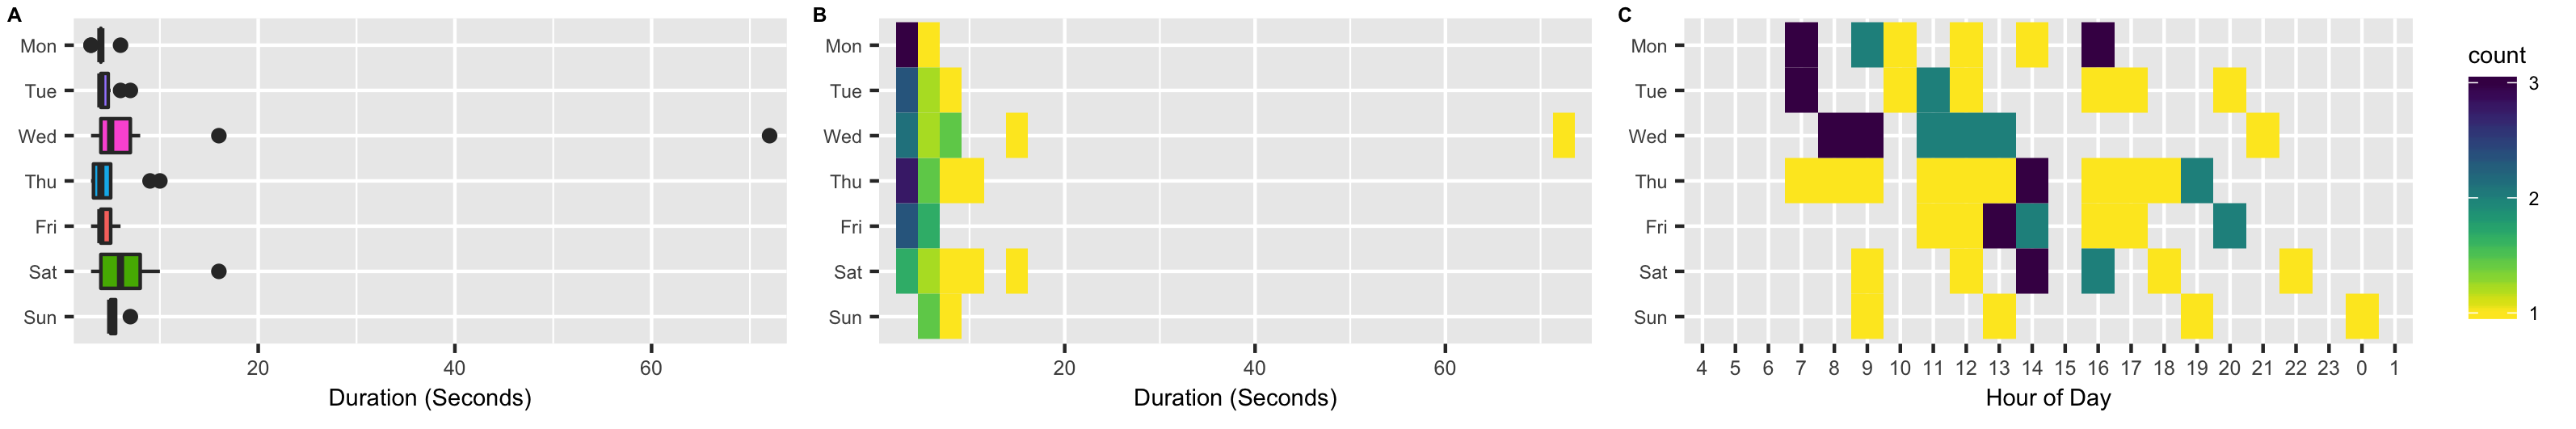
\includegraphics[width=1\linewidth]{/Users/alistairgj/Documents/GitHub/IoT_ResearchProject/IoT_November/images/subAct140} 

}

\caption{A caption}\label{fig:subAct140}
\end{figure}

\hypertarget{kitchen-freezer}{%
\paragraph{Kitchen Freezer}\label{kitchen-freezer}}

\begin{figure}[H]

{\centering 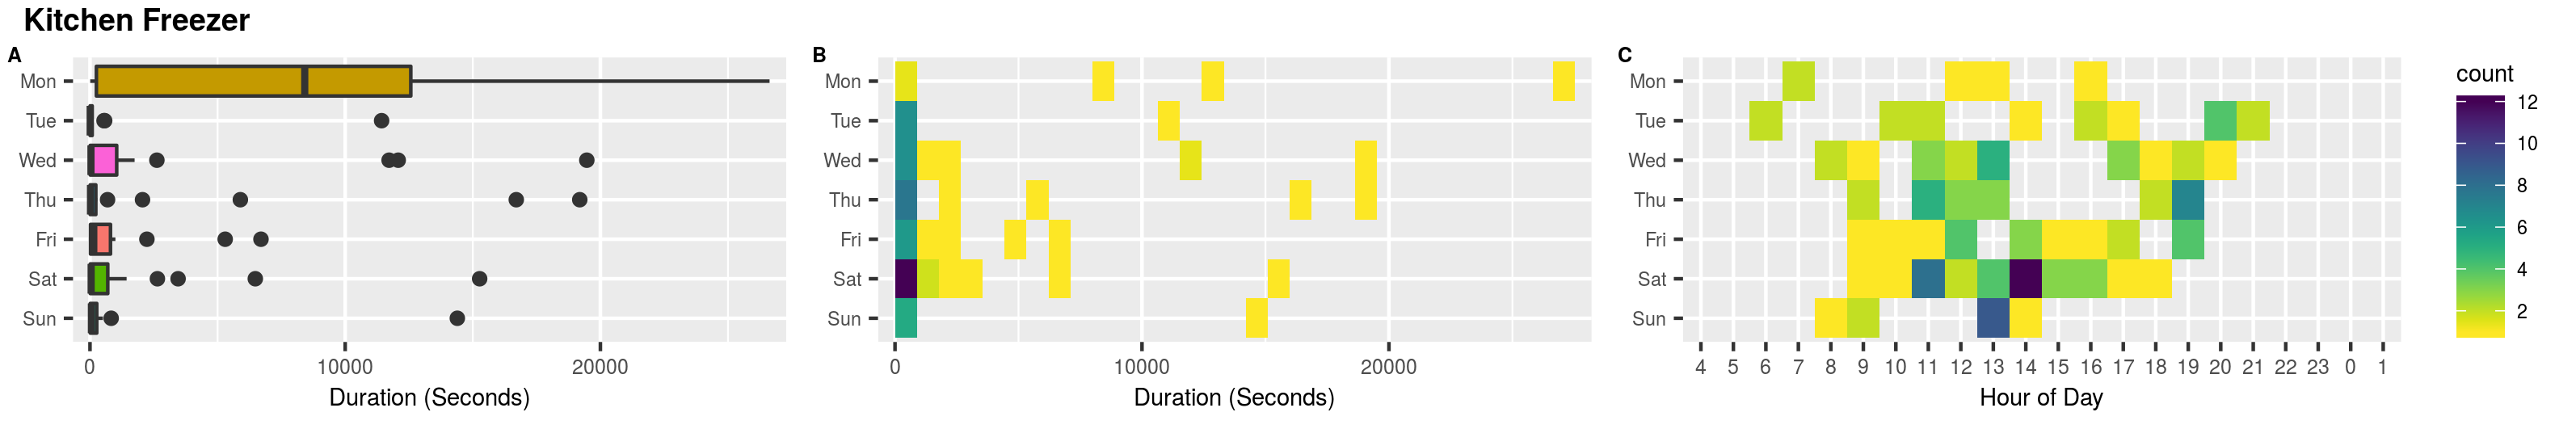
\includegraphics[width=1\linewidth]{/Users/alistairgj/Documents/GitHub/IoT_ResearchProject/IoT_November/images/subAct137} 

}

\caption{A caption}\label{fig:subAct137}
\end{figure}

\hypertarget{kitchen-burner}{%
\paragraph{Kitchen Burner}\label{kitchen-burner}}

\begin{figure}[H]

{\centering 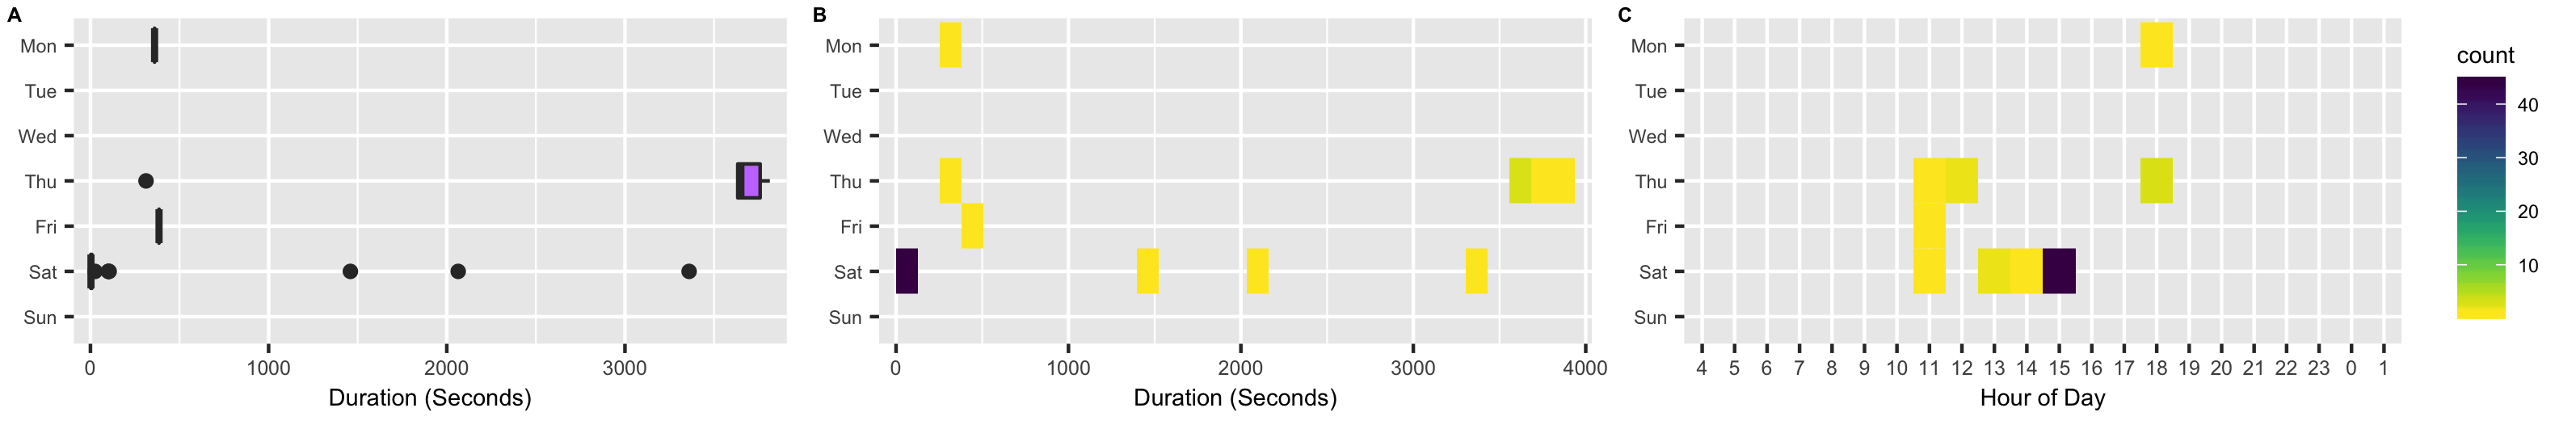
\includegraphics[width=1\linewidth]{/Users/alistairgj/Documents/GitHub/IoT_ResearchProject/IoT_November/images/subAct106} 

}

\caption{A caption}\label{fig:subAct106}
\end{figure}

\hypertarget{kitchen-lightswitch}{%
\paragraph{Kitchen Lightswitch}\label{kitchen-lightswitch}}

\begin{figure}[H]

{\centering 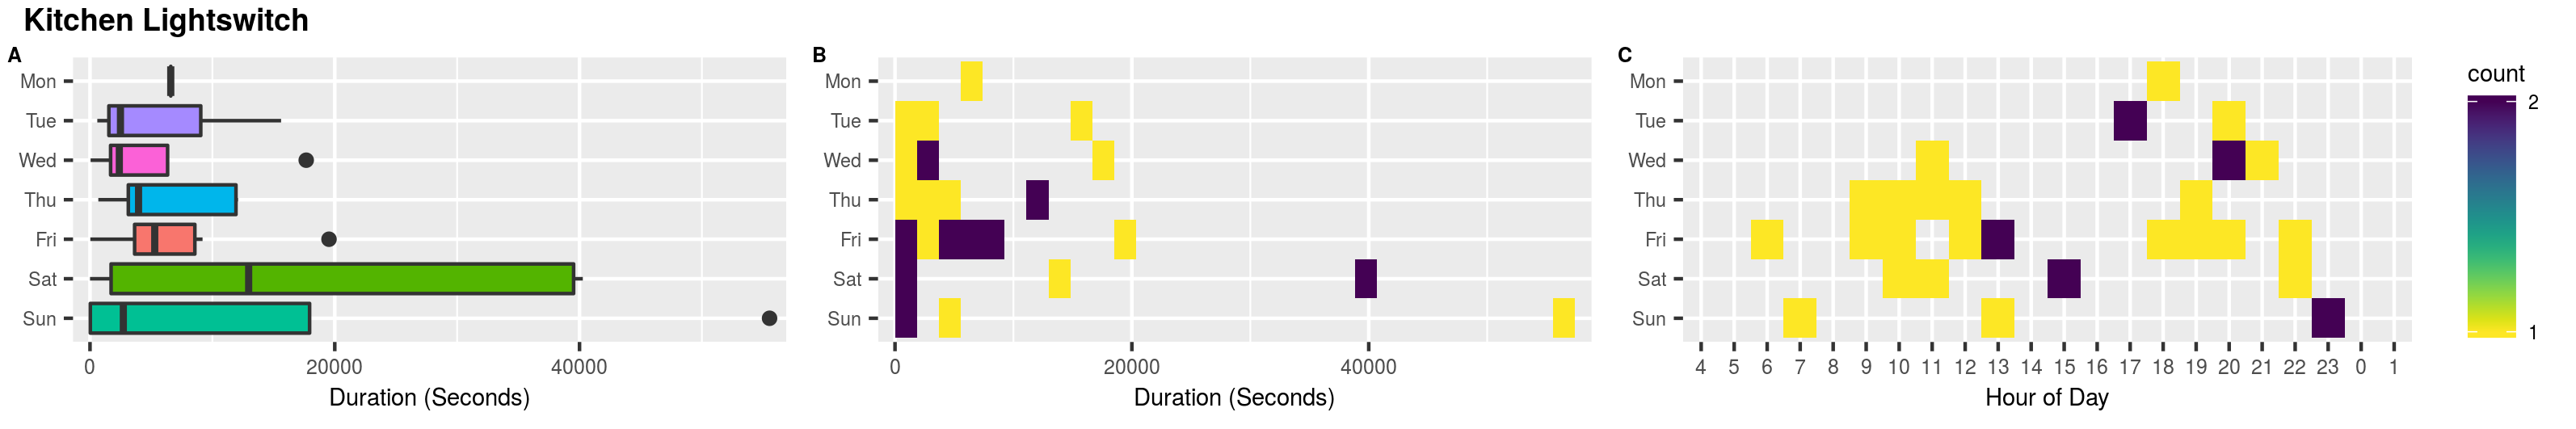
\includegraphics[width=1\linewidth]{/Users/alistairgj/Documents/GitHub/IoT_ResearchProject/IoT_November/images/subAct105} 

}

\caption{A caption}\label{fig:subAct105}
\end{figure}

\hypertarget{study-lightswitch-typo}{%
\paragraph{Study Lightswitch (TYPO)}\label{study-lightswitch-typo}}

\begin{figure}[H]

{\centering 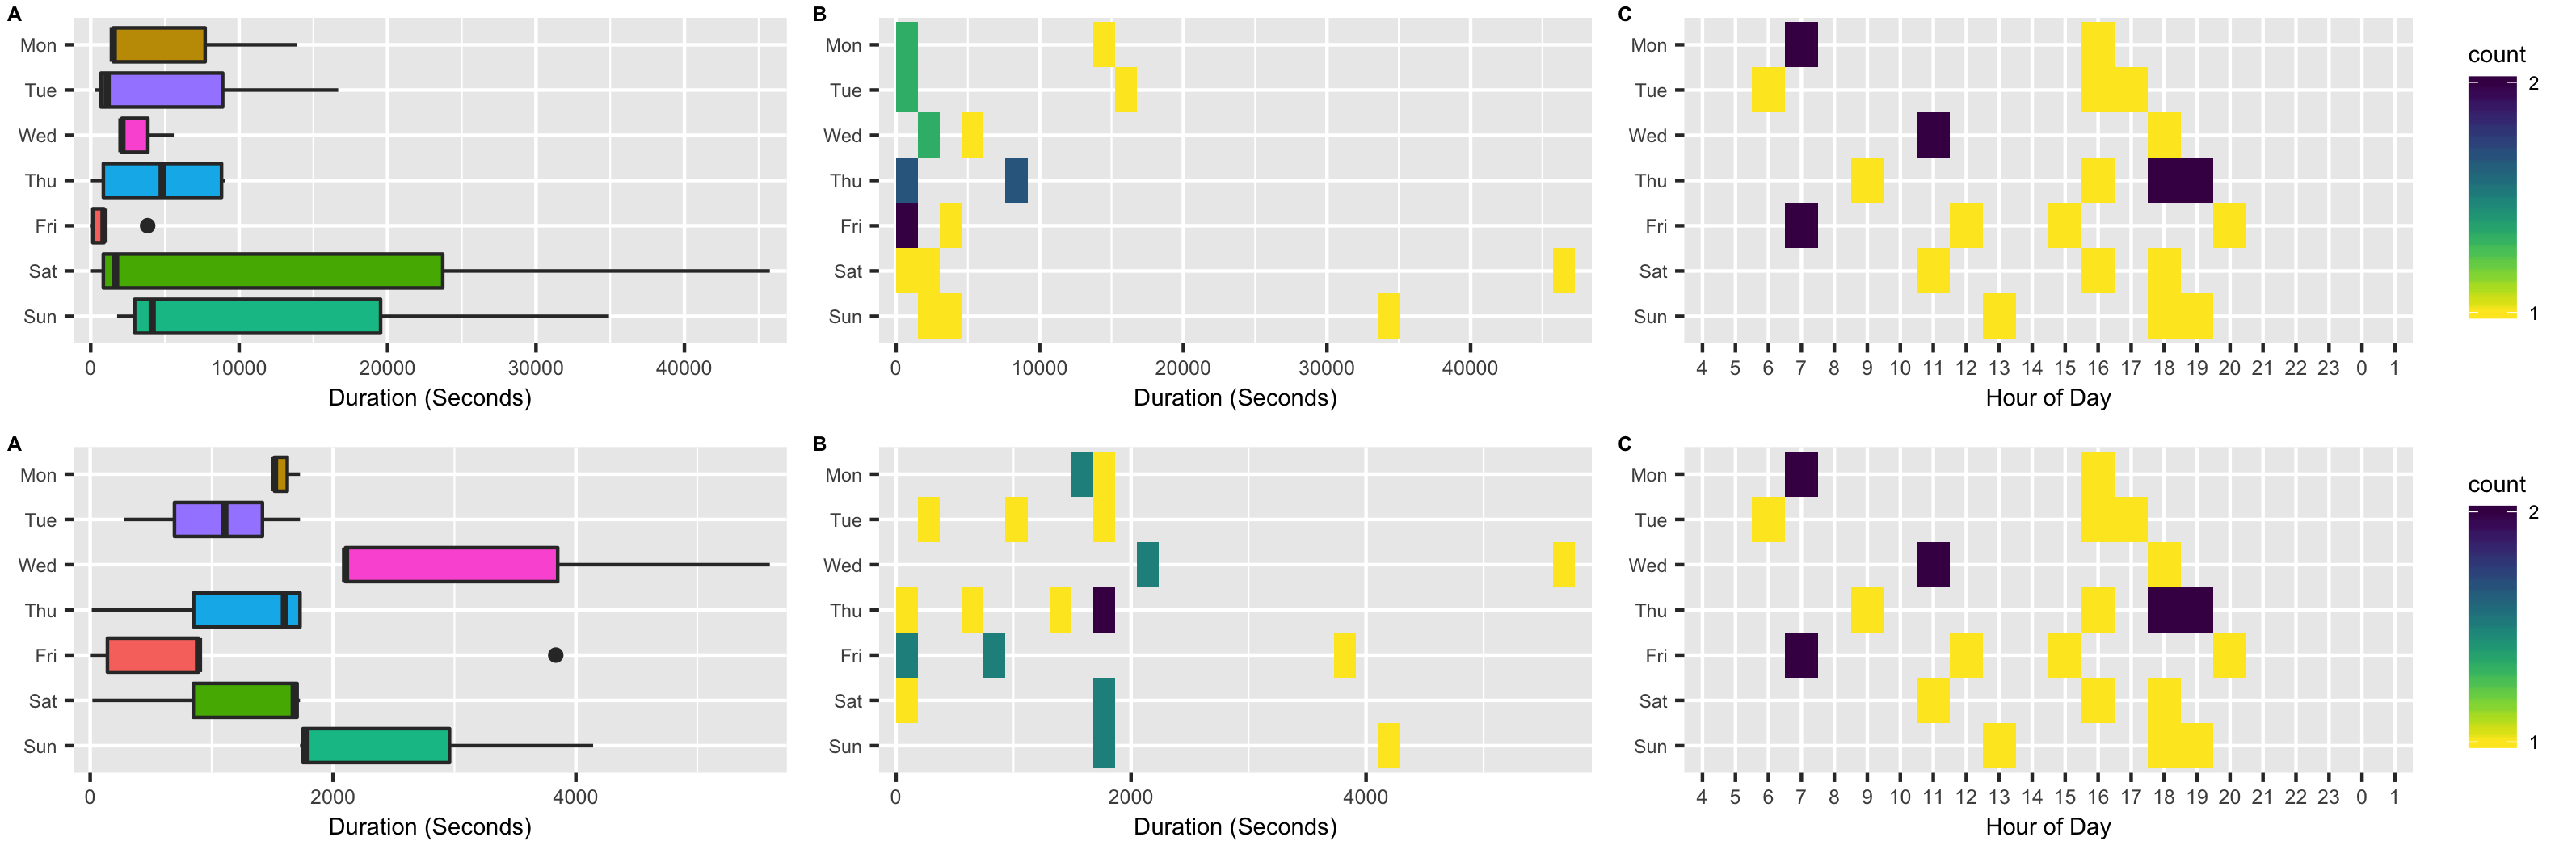
\includegraphics[width=1\linewidth]{/Users/alistairgj/Documents/GitHub/IoT_ResearchProject/IoT_November/images/subAct92} 

}

\caption{A caption}\label{fig:subAct92}
\end{figure}

\hypertarget{bathroom-door}{%
\paragraph{Bathroom Door}\label{bathroom-door}}

\begin{figure}[H]

{\centering 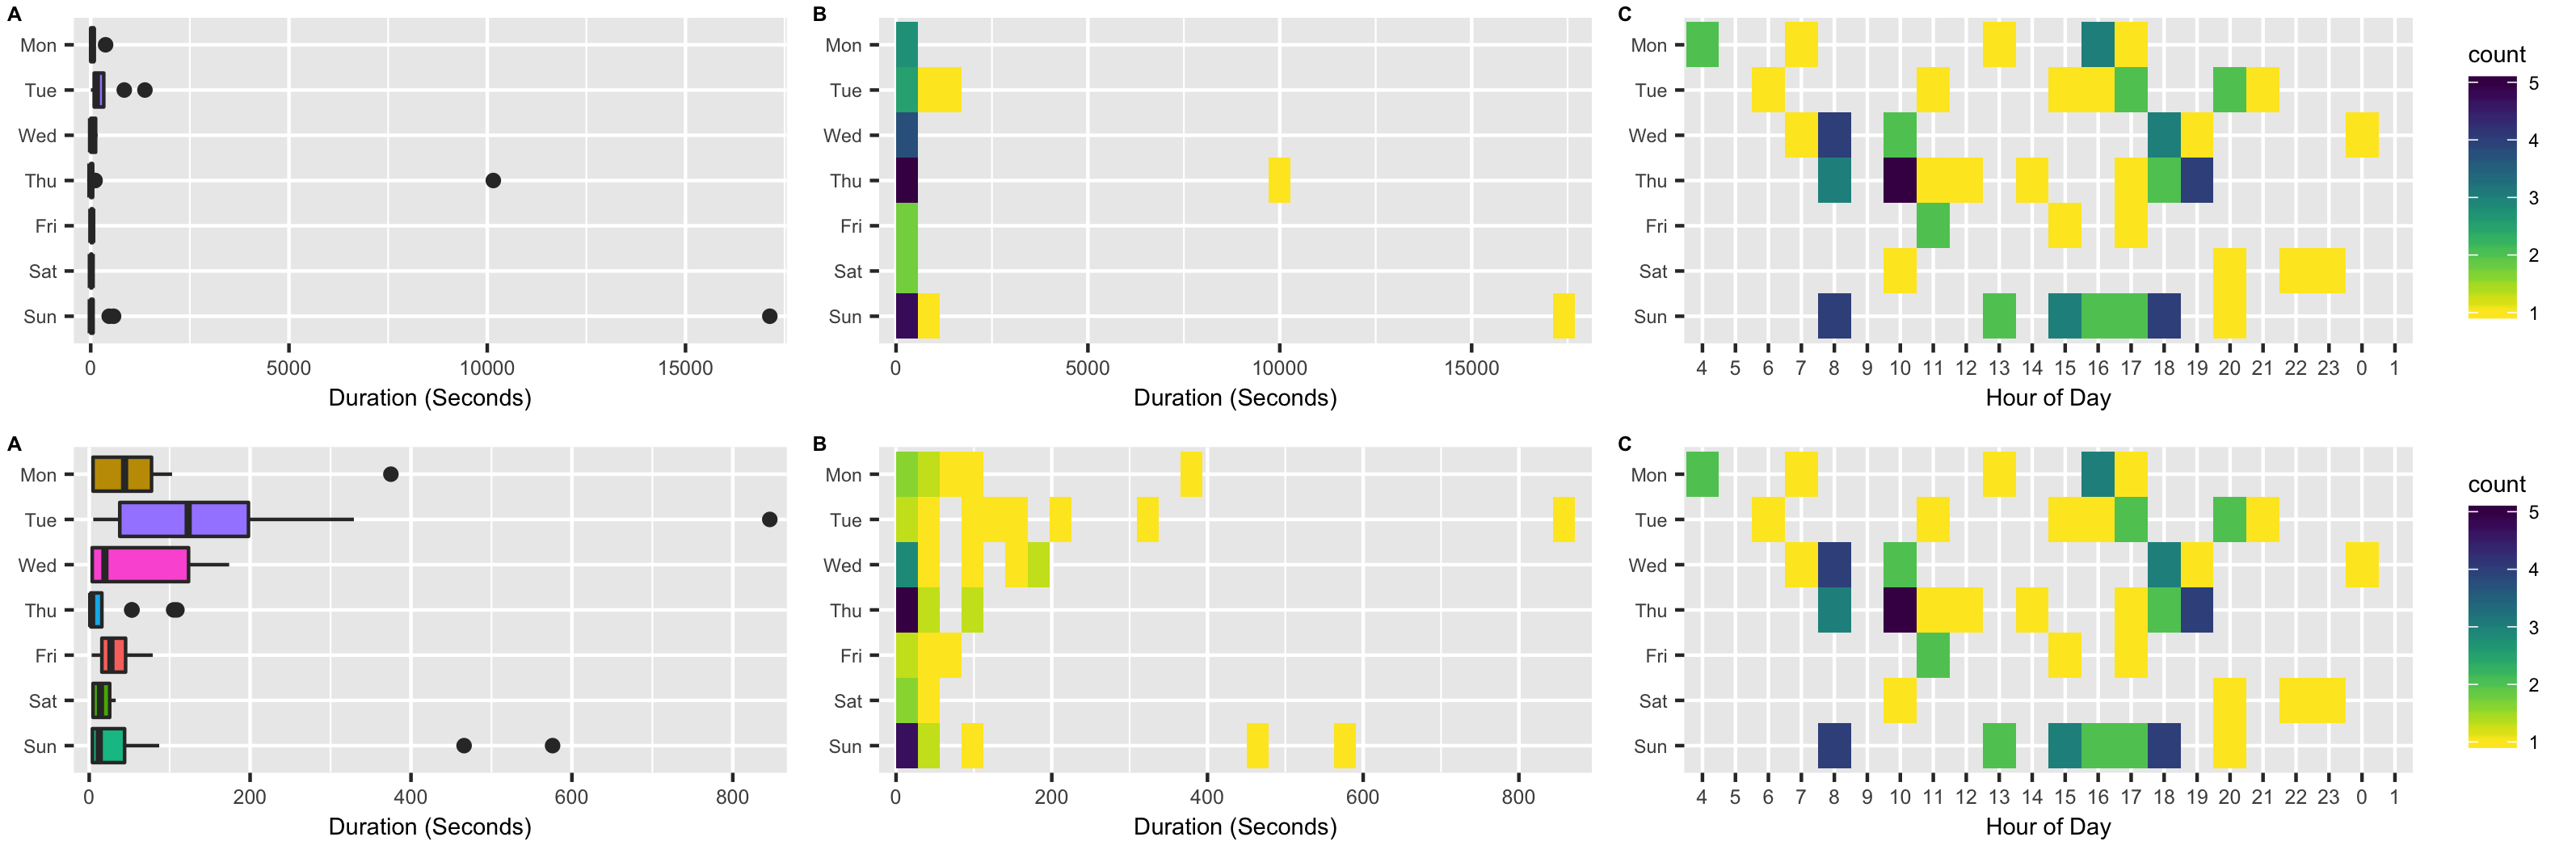
\includegraphics[width=1\linewidth]{/Users/alistairgj/Documents/GitHub/IoT_ResearchProject/IoT_November/images/subAct130} 

}

\caption{A caption}\label{fig:subAct130}
\end{figure}

\hypertarget{foyer-lightswitch}{%
\paragraph{Foyer Lightswitch}\label{foyer-lightswitch}}

\begin{figure}[H]

{\centering 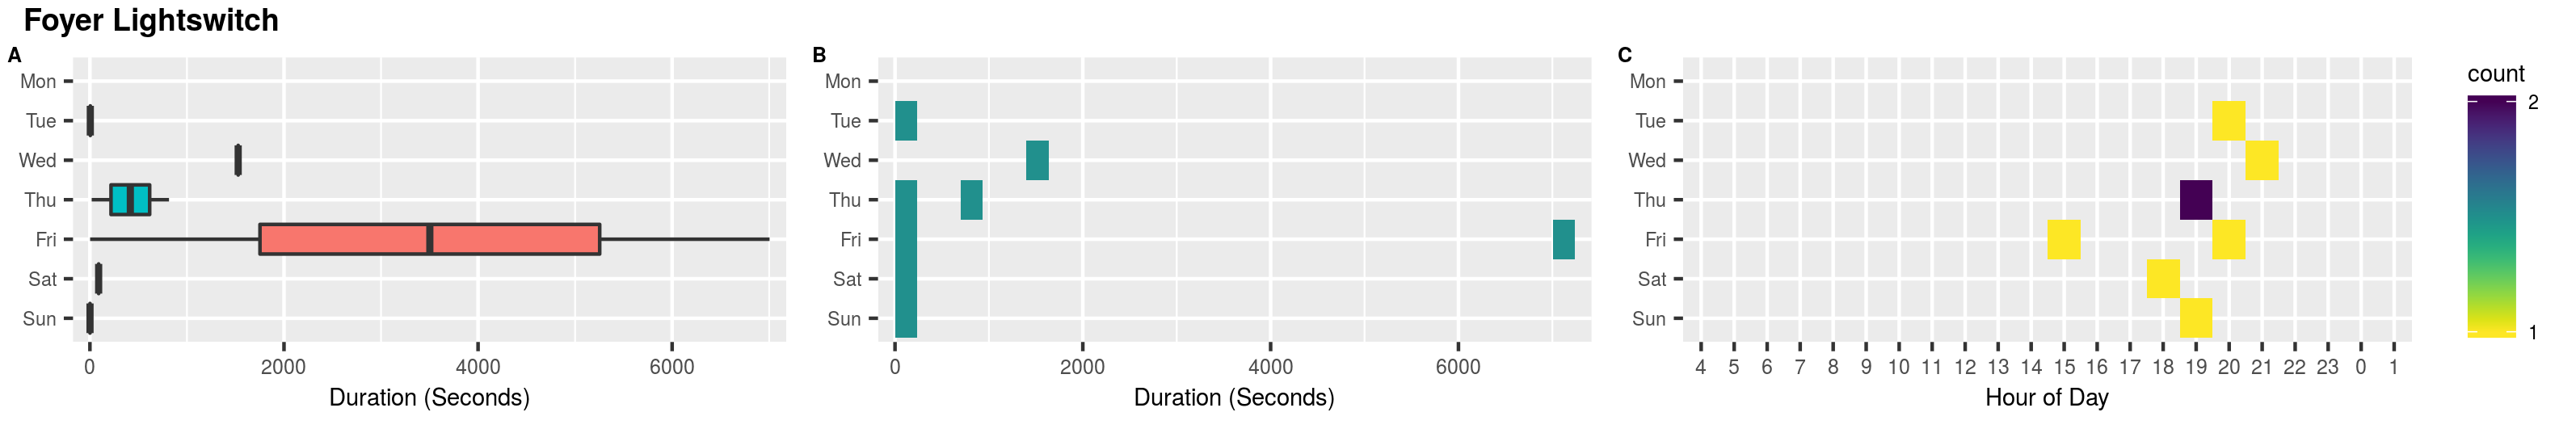
\includegraphics[width=1\linewidth]{/Users/alistairgj/Documents/GitHub/IoT_ResearchProject/IoT_November/images/subAct104} 

}

\caption{A caption}\label{fig:subAct104}
\end{figure}

\hypertarget{kitchen-toaster}{%
\paragraph{Kitchen Toaster}\label{kitchen-toaster}}

\begin{figure}[H]

{\centering \includegraphics[width=1\linewidth]{/Users/alistairgj/Documents/GitHub/IoT_ResearchProject/IoT_November/images/subAct131} 

}

\caption{A caption}\label{fig:subAct131}
\end{figure}

\hypertarget{bathroom-exhaust-fan}{%
\paragraph{Bathroom Exhaust Fan}\label{bathroom-exhaust-fan}}

\begin{figure}[H]

{\centering \includegraphics[width=1\linewidth]{/Users/alistairgj/Documents/GitHub/IoT_ResearchProject/IoT_November/images/subAct96} 

}

\caption{A caption}\label{fig:subAct96}
\end{figure}

\hypertarget{bedroom-lightswitch}{%
\paragraph{Bedroom Lightswitch}\label{bedroom-lightswitch}}

\begin{figure}[H]

{\centering \includegraphics[width=1\linewidth]{/Users/alistairgj/Documents/GitHub/IoT_ResearchProject/IoT_November/images/subAct108} 

}

\caption{A caption}\label{fig:subAct108}
\end{figure}

\hypertarget{kitchen-oven}{%
\paragraph{Kitchen Oven}\label{kitchen-oven}}

\begin{figure}[H]

{\centering \includegraphics[width=1\linewidth]{/Users/alistairgj/Documents/GitHub/IoT_ResearchProject/IoT_November/images/subAct129} 

}

\caption{A caption}\label{fig:subAct129}
\end{figure}

\hypertarget{livingroom-lamp}{%
\paragraph{Livingroom Lamp}\label{livingroom-lamp}}

\begin{figure}[H]

{\centering \includegraphics[width=1\linewidth]{/Users/alistairgj/Documents/GitHub/IoT_ResearchProject/IoT_November/images/subAct76} 

}

\caption{A caption}\label{fig:subAct76}
\end{figure}

\hypertarget{kitchen-washingmachine}{%
\paragraph{Kitchen Washingmachine}\label{kitchen-washingmachine}}

\begin{figure}[H]

{\centering \includegraphics[width=1\linewidth]{/Users/alistairgj/Documents/GitHub/IoT_ResearchProject/IoT_November/images/subAct142} 

}

\caption{A caption}\label{fig:subAct142}
\end{figure}

\hypertarget{kitchen-laundry-dryer}{%
\paragraph{Kitchen Laundry Dryer}\label{kitchen-laundry-dryer}}

\begin{figure}[H]

{\centering \includegraphics[width=1\linewidth]{/Users/alistairgj/Documents/GitHub/IoT_ResearchProject/IoT_November/images/subAct90} 

}

\caption{A caption}\label{fig:subAct90}
\end{figure}

\hypertarget{kitchen-garbage-disposal}{%
\paragraph{Kitchen Garbage Disposal}\label{kitchen-garbage-disposal}}

\begin{figure}[H]

{\centering \includegraphics[width=1\linewidth]{/Users/alistairgj/Documents/GitHub/IoT_ResearchProject/IoT_November/images/subAct98} 

}

\caption{A caption}\label{fig:subAct98}
\end{figure}

\hypertarget{livingroom-lightswitch}{%
\paragraph{Livingroom Lightswitch}\label{livingroom-lightswitch}}

\begin{figure}[H]

{\centering \includegraphics[width=1\linewidth]{/Users/alistairgj/Documents/GitHub/IoT_ResearchProject/IoT_November/images/subAct107} 

}

\caption{A caption}\label{fig:subAct107}
\end{figure}

\hypertarget{kitchen-cereal-subactnum-145}{%
\paragraph{Kitchen Cereal (SubActNum
145)}\label{kitchen-cereal-subactnum-145}}

DROPPED

\begin{figure}[H]

{\centering \includegraphics[width=1\linewidth]{/Users/alistairgj/Documents/GitHub/IoT_ResearchProject/IoT_November/images/subAct145} 

}

\caption{A caption}\label{fig:subAct145}
\end{figure}

\hypertarget{kitchen-containers-subactnum-60}{%
\paragraph{Kitchen Containers (SubActNum
60)}\label{kitchen-containers-subactnum-60}}

DROPPED

\begin{figure}[H]

{\centering \includegraphics[width=1\linewidth]{/Users/alistairgj/Documents/GitHub/IoT_ResearchProject/IoT_November/images/subAct60} 

}

\caption{A caption}\label{fig:subAct60}
\end{figure}

\hypertarget{kitchen-coffee-machine}{%
\paragraph{Kitchen Coffee Machine}\label{kitchen-coffee-machine}}

\begin{figure}[H]

{\centering \includegraphics[width=1\linewidth]{/Users/alistairgj/Documents/GitHub/IoT_ResearchProject/IoT_November/images/subAct119} 

}

\caption{A caption}\label{fig:subAct119}
\end{figure}

\hypertarget{bedroom-lamp-subactnum-64}{%
\paragraph{Bedroom Lamp (SubActNum
64)}\label{bedroom-lamp-subactnum-64}}

DROPPED

\begin{figure}[H]

{\centering \includegraphics[width=1\linewidth]{/Users/alistairgj/Documents/GitHub/IoT_ResearchProject/IoT_November/images/subAct64} 

}

\caption{A caption}\label{fig:subAct64}
\end{figure}

\begin{figure}[H]

{\centering \includegraphics{MD_Final_files/figure-latex/fig1-1} 

}

\caption{\label{fig:fig1}This is a caption}\label{fig:fig1}
\end{figure}

Reduce image border (not working???)
\url{https://holtzy.github.io/Pimp-my-rmd/}

S1SubActivities\_temporalFeaturesCLEANSED.csv = `Final' dataset

\hypertarget{algorithm-1}{%
\paragraph{Algorithm 1}\label{algorithm-1}}

Text

\begin{algorithm}[H]
\DontPrintSemicolon
\SetAlgoLined
\KwResult{Write here the result}
\SetKwInOut{Input}{Input}\SetKwInOut{Output}{Output}
\Input{Write here the input}
\Output{Write here the output}
\BlankLine
\While{While condition}{
    instructions\;
    \eIf{condition}{
        instructions1\;
        instructions2\;
    }{
        instructions3\;
    }
}
\caption{While loop with If/Else condition}
\end{algorithm}

\url{https://daattali.com/shiny/colourInput/}

\hypertarget{strip-plots}{%
\paragraph{Strip Plots}\label{strip-plots}}

\hypertarget{references}{%
\section*{References}\label{references}}
\addcontentsline{toc}{section}{References}

\hypertarget{refs}{}
\leavevmode\hypertarget{ref-pressAltairHistoryPersonal1993}{}%
1. Press L (1993) Before the Altair: The history of personal computing.
Commun ACM 36:27--33. \url{https://doi.org/10.1145/162685.162697}

\leavevmode\hypertarget{ref-duttaGlobalInformationTechnology2015}{}%
2. Dutta S, Geiger T, Lanvin B, et al (2015) The global information
technology report 2015: ICTs for inclusive growth

\leavevmode\hypertarget{ref-InformationCommunicationTechnologies}{}%
3. Information and communication technologies (ICTs) \textbar{} Poverty
Eradication.
\url{https://www.un.org/development/desa/socialperspectiveondevelopment/issues/information-and-communication-technologies-icts.html}.
Accessed 5 Nov 2019

\leavevmode\hypertarget{ref-DataNeverSleeps}{}%
4. Data Never Sleeps 5.0 \textbar{} Domo.
\url{https://www.domo.com/learn/data-never-sleeps-5?aid=ogsm072517_1\&sf100871281=1}.
Accessed 5 Nov 2019

\leavevmode\hypertarget{ref-CloudComputingDefinition}{}%
5. Cloud computing \textbar{} Definition of Cloud computing at
Dictionary.Com. \url{https://www.dictionary.com/browse/cloud-computing}.
Accessed 14 Nov 2019

\leavevmode\hypertarget{ref-danielemiorandiInternetThingsVision2012}{}%
6. Daniele Miorandi FDP Sabrina Sicari (2012) Internet of things:
Vision, applications and research challenges. Ad Hoc Networks
10:1497--1516. \url{https://doi.org/10.1016/j.adhoc.2012.02.016}

\leavevmode\hypertarget{ref-binghuangServiceOrientedComputing16th2018}{}%
7. Bing Huang AGN Athman Bouguettaya (2018) Service-Oriented Computing,
16th International Conference, ICSOC 2018, Hangzhou, China, November
12-15, 2018, Proceedings. 660--678.
\url{https://doi.org/10.1007/978-3-030-03596-9_48}

\leavevmode\hypertarget{ref-luigiatzoriInternetThingsSurvey2010}{}%
8. Luigi Atzori GM Antonio Iera (2010) The Internet of Things: A survey.
Computer Networks 54:2787--2805.
\url{https://doi.org/10.1016/j.comnet.2010.05.010}

\leavevmode\hypertarget{ref-intergovernmentalpanelonclimatechangeGlobalWarming2018}{}%
9. Intergovernmental Panel on Climate Change (2018) Global warming of
1.5°C

\leavevmode\hypertarget{ref-EnergyDemandSector}{}%
10. Energy demand by sector \textbar{} Energy economics \textbar{} Home.
In: BP global.
\url{https://www.bp.com/en/global/corporate/energy-economics/energy-outlook/demand-by-sector.html}.
Accessed 14 Nov 2019

\leavevmode\hypertarget{ref-Consumption}{}%
11. Consumption. \url{https://www.iea.org/statistics/kwes/consumption/}.
Accessed 14 Nov 2019

\leavevmode\hypertarget{ref-haseebDoesInformationCommunication2019}{}%
12. Haseeb A, Xia E, Saud S, et al (2019) Does information and
communication technologies improve environmental quality in the era of
globalization? An empirical analysis. Environ Sci Pollut Res
26:8594--8608. \url{https://doi.org/10.1007/s11356-019-04296-x}

\leavevmode\hypertarget{ref-hornePrivacyTechnologyNorms2015}{}%
13. Horne C, Darras B, Bean E, et al (2015) Privacy, technology, and
norms: The case of Smart Meters. Social Science Research 51:64--76.
\url{https://doi.org/10.1016/j.ssresearch.2014.12.003}

\leavevmode\hypertarget{ref-jui-shengchouCloudForecastingSystem2019}{}%
14. Jui-Sheng Chou N-ST (2019) Cloud forecasting system for monitoring
and alerting of energy use by home appliances. Applied Energy
249:166--177. \url{https://doi.org/10.1016/j.apenergy.2019.04.063}

\leavevmode\hypertarget{ref-graabSmartGridSmart2011}{}%
15. Graab AC (2011) The smart grid: A smart solution to a complicated
problem. William and Mary Law Review 52:2051

\leavevmode\hypertarget{ref-charlotteb.a.kobusReallifeAssessmentEffect2015}{}%
16. Charlotte B. A. Kobus RM Elke A. M. Klaassen (2015) A real-life
assessment on the effect of smart appliances for shifting households'
electricity demand. Applied Energy 147:335--343.
\url{https://doi.org/10.1016/j.apenergy.2015.01.073}

\leavevmode\hypertarget{ref-k.s.cetinApplianceDailyEnergy2014}{}%
17. K. S. Cetin AN P. C. Tabares-Velasco (2014) Appliance daily energy
use in new residential buildings: Use profiles and variation in
time-of-use. Energy and Buildings 84:716--726.
\url{https://doi.org/10.1016/j.enbuild.2014.07.045}

\leavevmode\hypertarget{ref-kaustavbasuApplianceUsagePrediction2012}{}%
18. Kaustav Basu SB Vincent Debusschere (2012) Appliance usage
prediction using a time series based classification approach.
1217--1222. \url{https://doi.org/10.1109/iecon.2012.6388597}

\leavevmode\hypertarget{ref-d.m.murrayApplianceElectricalConsumption2018}{}%
19. D. M. Murray VS L. Stankovic (2018) Appliance electrical consumption
modelling at scale using smart meter data. Journal of Cleaner
Production. \url{https://doi.org/10.1016/j.jclepro.2018.03.163}

\leavevmode\hypertarget{ref-rockinsonActivityRecognitionHome}{}%
20. Rockinson R Activity Recognition in the Home Setting Using Simple
and Ubiquitous sensors

\leavevmode\hypertarget{ref-countrycode}{}%
21. Arel-Bundock V, Enevoldsen N, Yetman C (2018) Countrycode: An r
package to convert country names and country codes. Journal of Open
Source Software 3:848

\leavevmode\hypertarget{ref-cowplot}{}%
22. Wilke CO (2018) Cowplot: Streamlined plot theme and plot annotations
for 'ggplot2'

\leavevmode\hypertarget{ref-bibtex}{}%
23. Francois R (2017) Bibtex: Bibtex parser

\leavevmode\hypertarget{ref-dplyr}{}%
24. Wickham H, François R, Henry L, Müller K (2019) Dplyr: A grammar of
data manipulation

\leavevmode\hypertarget{ref-ggExtra}{}%
25. Attali D, Baker C (2018) GgExtra: Add marginal histograms to
'ggplot2', and more 'ggplot2' enhancements

\leavevmode\hypertarget{ref-tidyverse}{}%
26. Wickham H (2017) Tidyverse: Easily install and load the 'tidyverse'

\leavevmode\hypertarget{ref-ggplot2}{}%
27. Wickham H (2016) Ggplot2: Elegant graphics for data analysis.
Springer-Verlag New York

\leavevmode\hypertarget{ref-ggridges}{}%
28. Wilke CO (2018) Ggridges: Ridgeline plots in 'ggplot2'

\leavevmode\hypertarget{ref-kableExtra}{}%
29. Zhu H (2018) KableExtra: Construct complex table with 'kable' and
pipe syntax

\leavevmode\hypertarget{ref-knitr1}{}%
30. Xie Y (2019) Knitr: A general-purpose package for dynamic report
generation in r

\leavevmode\hypertarget{ref-lubridate}{}%
31. Grolemund G, Wickham H (2011) Dates and times made easy with
lubridate. Journal of Statistical Software 40:1--25

\leavevmode\hypertarget{ref-readr}{}%
32. Wickham H, Hester J, Francois R (2017) Readr: Read rectangular text
data

\leavevmode\hypertarget{ref-tidyr}{}%
33. Wickham H, Henry L (2018) Tidyr: Easily tidy data with 'spread()'
and 'gather()' functions

\leavevmode\hypertarget{ref-viridis}{}%
34. Garnier S (2018) Viridis: Default color maps from 'matplotlib'

\leavevmode\hypertarget{ref-reticulate}{}%
35. Ushey K, Allaire J, Tang Y (2019) Reticulate: Interface to 'python'

\leavevmode\hypertarget{ref-ggsci}{}%
36. Xiao N (2017) Ggsci: Scientific journal and sci-fi themed color
palettes for 'ggplot2'

\leavevmode\hypertarget{ref-scales}{}%
37. Wickham H (2018) Scales: Scale functions for visualization


\end{document}
